%%%%%%%%%%%%%%%%%%%%%%%%%%%%%%%%%%%%%%%%%
% Masters/Doctoral Thesis 
% LaTeX Template
% Version 2.5 (27/8/17)
%
% This template was downloaded from:
% http://www.LaTeXTemplates.com
%
% Version 2.x major modifications by:
% Vel (vel@latextemplates.com)
%
% This template is based on a template by:
% Steve Gunn (http://users.ecs.soton.ac.uk/srg/softwaretools/document/templates/)
% Sunil Patel (http://www.sunilpatel.co.uk/thesis-template/)
%
% Template license:
% CC BY-NC-SA 3.0 (http://creativecommons.org/licenses/by-nc-sa/3.0/)
%
%%%%%%%%%%%%%%%%%%%%%%%%%%%%%%%%%%%%%%%%%

%----------------------------------------------------------------------------------------
%	PACKAGES AND OTHER DOCUMENT CONFIGURATIONS
%----------------------------------------------------------------------------------------

\documentclass[
11pt, % The default document font size, options: 10pt, 11pt, 12pt
oneside, % Two side (alternating margins) for binding by default, uncomment to switch to one side
english, % ngerman for German
singlespacing, % Single line spacing, alternatives: onehalfspacing or doublespacing
%draft, % Uncomment to enable draft mode (no pictures, no links, overfull hboxes indicated)
%nolistspacing, % If the document is onehalfspacing or doublespacing, uncomment this to set spacing in lists to single
%liststotoc, % Uncomment to add the list of figures/tables/etc to the table of contents
%toctotoc, % Uncomment to add the main table of contents to the table of contents
%parskip, % Uncomment to add space between paragraphs
%nohyperref, % Uncomment to not load the hyperref package
headsepline, % Uncomment to get a line under the header
chapterinoneline, % Uncomment to place the chapter title next to the number on one line
%consistentlayout, % Uncomment to change the layout of the declaration, abstract and acknowledgements pages to match the default layout
]{MastersDoctoralThesis} % The class file specifying the document structure

\usepackage[utf8]{inputenc} % Required for inputting international characters
\usepackage[T1]{fontenc} % Output font encoding for international characters

\usepackage{mathpazo} % Use the Palatino font by default
\usepackage[
backend=biber,
style=numeric,
sorting=ynt
]{biblatex}

%\usepackage[backend=bibtex,style=authoryear,natbib=true]{biblatex} % Use the bibtex backend with the authoryear citation style (which resembles APA)

\addbibresource{References.bib} % The filename of the bibliography

\usepackage[autostyle=true]{csquotes} % Required to generate language-dependent quotes in the bibliography

%My own settings
\usepackage{comment}
\usepackage{float}
\usepackage{pdfpages}
%\usepackage{titlesec}

%\titleformat{\chapter}
%{\Large\bfseries} % format
%{}                % label
%{0pt}             % sep
%{\huge}           % before-code
  
%----------------------------------------------------------------------------------------
%	MARGIN SETTINGS
%----------------------------------------------------------------------------------------

\geometry{
	paper=a4paper, % Change to letterpaper for US letter
	inner=2.5cm, % Inner margin
	outer=3.8cm, % Outer margin
	bindingoffset=.5cm, % Binding offset
	top=1.5cm, % Top margin
	bottom=1.5cm, % Bottom margin
	%showframe, % Uncomment to show how the type block is set on the page
}

%----------------------------------------------------------------------------------------
%	THESIS INFORMATION
%----------------------------------------------------------------------------------------

\thesistitle{Graph generation and route planning in BIM models} % Your thesis title, this is used in the title and abstract, print it elsewhere with \ttitle
\supervisor{Associate professor Jakob Andreas Bærentzen} % Your supervisor's name, this is used in the title page, print it elsewhere with \supname
\examiner{} % Your examiner's name, this is not currently used anywhere in the template, print it elsewhere with \examname
\degree{Master of Science in Engineering} % Your degree name, this is used in the title page and abstract, print it elsewhere with \degreename
\author{Kia Kafaei Yahyavi} % Your name, this is used in the title page and abstract, print it elsewhere with \authorname
\addresses{} % Your address, this is not currently used anywhere in the template, print it elsewhere with \addressname

%\subject{Biological Sciences} % Your subject area, this is not currently used anywhere in the template, print it elsewhere with \subjectname
\keywords{} % Keywords for your thesis, this is not currently used anywhere in the template, print it elsewhere with \keywordnames
\university{\href{https://www.dtu.dk/}{Technical University of Denmark}} % Your university's name and URL, this is used in the title page and abstract, print it elsewhere with \univname
\department{\href{https://www.dtu.dk/english/Education/msc/Programmes/mathematical_modelling_and_computation}{Mathematical Modelling and Computation}} % Your department's name and URL, this is used in the title page and abstract, print it elsewhere with \deptname
%\group{\href{http://researchgroup.university.com}{Research Group Name}} % Your research group's name and URL, this is used in the title page, print it elsewhere with \groupname
\faculty{\href{https://www.dtu.dk/english/Education/msc/Programmes/mathematical_modelling_and_computation}{Mathematical Modelling and Computation}} % Your faculty's name and URL, this is used in the title page and abstract, print it elsewhere with \facname

\AtBeginDocument{
\hypersetup{pdftitle=\ttitle} % Set the PDF's title to your title
\hypersetup{pdfauthor=\authorname} % Set the PDF's author to your name
\hypersetup{pdfkeywords=\keywordnames} % Set the PDF's keywords to your keywords
}

\begin{document}

\frontmatter % Use roman page numbering style (i, ii, iii, iv...) for the pre-content pages

\pagestyle{plain} % Default to the plain heading style until the thesis style is called for the body content

%----------------------------------------------------------------------------------------
%	TITLE PAGE
%----------------------------------------------------------------------------------------

\begin{titlepage}
\begin{center}

\vspace*{.06\textheight}
{\scshape\LARGE \univname\par}\vspace{1.5cm} % University name
\textsc{\Large Master Thesis}\\[0.5cm] % Thesis type

\HRule \\[0.4cm] % Horizontal line
{\huge \bfseries \ttitle\par}\vspace{0.4cm} % Thesis title
\HRule \\[1.5cm] % Horizontal line
 
\begin{minipage}[t]{0.4\textwidth}
\begin{flushleft} \large
\emph{Author:}\\
%\href{http://www.johnsmith.com}{
\authorname % Author name - remove the \href bracket to remove the link
\end{flushleft}
\end{minipage}
\begin{minipage}[t]{0.4\textwidth}
\begin{flushright} \large
\emph{Supervisor:} \\
\href{https://www.inside.dtu.dk/en/dtuinside/generelt/telefonbog/person?id=4465&cpid=&tab=1}{\supname} % Supervisor name - remove the \href bracket to remove the link  
\end{flushright}
\end{minipage}\\[3cm]
 
\vfill

\large \textit{A thesis submitted in fulfillment of the requirements\\ for the degree of \degreename}\\[0.3cm] % University requirement text
\textit{in the department of}\\[0.4cm]
\groupname\\\deptname\\[2cm] % Research group name and department name
\vfill

{\large \today}\\[4cm] % Date
%\includegraphics{Logo} % University/department logo - uncomment to place it
 
\vfill
\end{center}
\end{titlepage}

%----------------------------------------------------------------------------------------
%	DECLARATION PAGE
%----------------------------------------------------------------------------------------

\begin{declaration}
\addchaptertocentry{\authorshipname} % Add the declaration to the table of contents
\noindent I, \authorname, declare that this thesis titled, \enquote{\ttitle} and the work presented in it are my own. I confirm that:

\begin{itemize} 
\item This work was done wholly or mainly while in candidature for a Master's degree at this University.
\item Where any part of this thesis has previously been submitted for a degree or any other qualification at this University or any other institution, this has been clearly stated.
\item Where I have consulted the published work of others, this is always clearly attributed.
\item Where I have quoted from the work of others, the source is always given. With the exception of such quotations, this thesis is entirely my own work.
\item I have acknowledged all main sources of help.
\item Where the thesis is based on work done by myself jointly with others, I have made clear exactly what was done by others and what I have contributed myself.\\
\end{itemize}
 
\noindent Signed:\\
\rule[0.5em]{25em}{0.5pt} % This prints a line for the signature
 
\noindent Date:\\
\rule[0.5em]{25em}{0.5pt} % This prints a line to write the date
\end{declaration}

\cleardoublepage

%----------------------------------------------------------------------------------------
%	QUOTATION PAGE
%----------------------------------------------------------------------------------------

%\vspace*{0.2\textheight}

%\noindent\enquote{\itshape Thanks to my solid academic training, today I can write hundreds of words on virtually any topic without possessing a shred of information, which is how I got a good job in journalism.}\bigbreak

%\hfill Dave Barry

%----------------------------------------------------------------------------------------
%	ABSTRACT PAGE
%----------------------------------------------------------------------------------------

\begin{abstract}
\addchaptertocentry{\abstractname} % Add the abstract to the table of contents
The Thesis Abstract is written here (and usually kept to just this page). The page is kept centered vertically so can expand into the blank space above the title too\ldots
\end{abstract}

%----------------------------------------------------------------------------------------
%	ACKNOWLEDGEMENTS
%----------------------------------------------------------------------------------------

%\begin{acknowledgements}
%\addchaptertocentry{\acknowledgementname} % Add the acknowledgements to the table of contents
%The acknowledgments and the people to thank go here, don't forget to include your project advisor\ldots
%\end{acknowledgements}

%----------------------------------------------------------------------------------------
%	LIST OF CONTENTS/FIGURES/TABLES PAGES
%----------------------------------------------------------------------------------------

\tableofcontents % Prints the main table of contents

%\listoffigures % Prints the list of figures

%\listoftables % Prints the list of tables

%----------------------------------------------------------------------------------------
%	ABBREVIATIONS
%----------------------------------------------------------------------------------------

%\begin{abbreviations}{ll} % Include a list of abbreviations (a table of two columns)

%\textbf{LAH} & \textbf{L}ist \textbf{A}bbreviations \textbf{H}ere\\
%\textbf{WSF} & \textbf{W}hat (it) \textbf{S}tands \textbf{F}or\\

%\end{abbreviations}

%----------------------------------------------------------------------------------------
%	PHYSICAL CONSTANTS/OTHER DEFINITIONS
%----------------------------------------------------------------------------------------

%\begin{constants}{lr@{${}={}$}l} % The list of physical constants is a three column table

% The \SI{}{} command is provided by the siunitx package, see its documentation for instructions on how to use it

%Speed of Light & $c_{0}$ & \SI{2.99792458e8}{\meter\per\second} (exact)\\
%Constant Name & $Symbol$ & $Constant Value$ with units\\

%\end{constants}

%----------------------------------------------------------------------------------------
%	SYMBOLS
%----------------------------------------------------------------------------------------

%\begin{symbols}{lll} % Include a list of Symbols (a three column table)

%$a$ & distance & \si{\meter} \\
%$P$ & power & \si{\watt} (\si{\joule\per\second}) \\
%Symbol & Name & Unit \\

%\addlinespace % Gap to separate the Roman symbols from the Greek

%$\omega$ & angular frequency & \si{\radian} \\

%\end{symbols}

%----------------------------------------------------------------------------------------
%	DEDICATION
%----------------------------------------------------------------------------------------

%\dedicatory{For/Dedicated to/To my\ldots} 

%----------------------------------------------------------------------------------------
%	THESIS CONTENT - CHAPTERS
%----------------------------------------------------------------------------------------

\mainmatter % Begin numeric (1,2,3...) page numbering

\pagestyle{thesis} % Return the page headers back to the "thesis" style

% Include the chapters of the thesis as separate files from the Chapters folder
% Uncomment the lines as you write the chapters

%\begin{document}
\large
%
\begin{titlepage}

%\begin{flushright}
%
\includegraphics[width=30mm]{billeder/dtulogo.png}
%\end{flushright}

\begin{center}
    
\vspace{10mm}
\noindent {\LARGE \textbf{ Master Thesis}}
\vspace{5mm}\\


\begin{figure}[t]
    \vspace*{-1cm}
    \hspace{14 cm}
    
\includegraphics[scale=0.1]{fig/dtulogo.png}
\end{figure}

\noindent { \large \textbf{
}}

\noindent { \large \textbf{Technical University of Denmark}}
%\line(1,0){\textwidth}

\vspace{5mm}

Navigerbarhed med BIM modeller

\noindent { \large \textbf{\today}}

% \vspace{15mm}
% \noindent {\large \textbf{\underline{\textbf{GROUP 14}}}}

\vspace{5mm}
Kia Kafaei Yahyavi

\end{center}

\vspace{29mm}

% \begin{figure}[H]
%     \hspace*{-2.7cm}
%     \includegraphics[scale = 0.9]{DTUBanner.png}
%     \vspace*{-0.1 cm}
% \end{figure}

\end{titlepage}




%\tableofcontents
\newpage
%\section{Different sections to write about}

\subsection{Previous work}
\begin{itemize}
    \item Write about the 3 week project Gwayfinding
\end{itemize}

\subsection{Litteratur review}
\begin{itemize}
    \item Write about the paper that explains people pathfinding in building, where they use grid instead of polygonal
    \item Write about pathfinding in 2d world master thesis. How they describe the difference between polygonal and grid, what algorithms to use for each etc.
    \item Write about the TSP problem, and its solutions. Find paper for that perhaps.
    \item Maybe find paper about Spot.
\end{itemize}


\subsection{Plotting floorplans}
\begin{itemize}
    \item Section about preprocessing of the dataset
    \item Section about the data and the polygonal triangle structure of the dataset, and why it makes sense.
    \item Talk about removing redundant lines from triangles.
    \item Talk about the challenges of plotting the doors. How I did this manually instead.
\end{itemize}

\subsection{Grid vs polygonal}
\begin{itemize}
    \item Talk about how you could use the grid version or the polygonal version. Spent a good amount of effort here.
\end{itemize}

\subsection{Which platform to use}
\begin{itemize}
    \item Write about which platform to use. The pros and cons of each. Ros vs Unity vs Python.
\end{itemize}


\subsection{TSP}
\begin{itemize}
    \item How to represent nodes and graphs? Comparison of different ways and libraries
    \item Making a weighted graph of all the nodes, where the weights are the Euclidean distance between each node. Write that it is a undirected graph.
    \item A section on the line intersection algorithm used for connecting the points
    \item Using dijkstra's/A* to make a complete subgraph of all the relevant nodes, and how this problem is a bit different than the traditional tsp.
    \item A section of the 2-OPT algorithm and how it uses Minimum Spanning Tree and a DFS traversal. You can talk about alternative algorithms and ther pros and cons.
    \item A section describing the MST and DFS algorithms and how Networkx implementation work. Maybe a section about adjacency list vs matrix, kruskal vs prims. When to use which.
\end{itemize}

\subsection{Dimensions of robot}
\begin{itemize}
    \item Write about how to incorporate the dimensions of the robot in your simulation
\end{itemize}

\subsection{Optimal placement of nodes}
\begin{itemize}
    \item Write about scenic route vs discrete points.
    \item Write about SLAM
    \item optimal placement of nodes
\end{itemize}

\subsection{Spot}
\begin{itemize}
    \item Write about Spot and how it is a usefull robot for this thesis
    \item Write about different platforms for programming Spot, python API vs ROS.
\end{itemize}

\subsection{Future work}
\begin{itemize}
    \item A section about stairs
\end{itemize}
\chapter{Introduction}
\section{Introduction}
Robots has been a thing of the future for a very long time being something only depicted in Hollywood movies with not much basis in reality. This fact is slowly changing and now we are seeing robots that are slowly looking like stuff from movies. 
The spot robot from Boston dynamics is the newest example of this. The spot robot is a yellow quadruped robot which literally looks like something taken from a movie.[insert reference to the black mirror episode].

At the same time the construction business needs a robot 

A lot of uses are being found for the robot one of which is in the construction industry. Which leads us to the motivation of this project.


\section{Motivation}
The project is being worked on in collaboration with Dalux which is a software company that makes BIM models (Building information modelling) for entrepreneurs making the construction process more manageable for them. 
Dalux has a desire to help the entrepreneurs get a better overview of what is being done on their construction site on a day to day basis; is a new wall being constructed, are some tubes being assembled etc. 
Dalux essentially wants to give a temporal overview of the construction process to the entrepreneur, while also precisely showing the entrepreneur if the work being done by his employees or contractors are done correctly.
He can use this information to hold his employees or contractors accountable; is the wall being placed where it should be placed, are the tubes being assembled correctly.

At present Dalux has to hire an expensive architect to walk around the construction site and check that everything is going according to plan and that there are not any errors occurring. Needless to say this is a costly affair.
This is where the SPOT robot enters the picture. Because if this process could be automated such that a robot could walk around a construction site instead and do point scans, send the data directly to Dalux’ software, that would be of great benefit for Dalux. 

This might save them a lot of effort and money, since a robot has a big upfront cost but a very small hourly work cost.


\section{Objective}\label{Objective} 
The objective of this project is to make a path-finding algorithm for the spot robot from Boston dynamics on the floor of a given building. The program should be able to get as input CAD data for a one level floor-plan of a building and should from that, output the path that the robot should traverse. The path should take into consideration the dimensions of the robot, such that it does not walk into walls or such that the planned path is not too narrow for the robot.


The path should be in the form of a loop, such that the start and end destinations of the path are the same - such that the robot can be put into the charger the following morning.


The path should furthermore guarantee that the robot visits every room on the floor.
\\\\
\textbf{How will this be done?}
%\subsubsection{How will this be done?}
\\
It makes sense to split this objective into 3 distinct problem definitions:
\begin{enumerate}
    \item \textbf{Making a graph - which we will denote “grid”- graph - from the input data.} From the CAD input we will sample nodes with a given resolution resulting in a discretized floor plan, denoted “grid”-graph. The walls of the floor plan will also be included for visual purposes. The graph is processed in such a way that the robot will always be able to traverse between two nodes in the floor plan if the nodes are connected; either directly or through intermediary nodes.
    
    \item \textbf{Making a subgraph - which we will denote “room”-graph - from the “grid”-graph.}
    The essential nodes that the robot must visit - to get to every room - will be generated, denoted as “room” nodes.

    A subgraph of the “grid”-graph will be generated where only the “room” nodes are included, denoted “room”- graph.
    An optimal graph traversal algorithm (e.g A* ) will be used to find the shortest distance between each node in this subgraph. An important property of this subgraph will be that it is fully connected; this means that all room nodes are connected to each other.

    
    \item \textbf{Making a path that traverses through all “room” nodes in the “grid” graph.} We will find an approximate solution to the traveling salesman problem on the “room” graph. This solution will be used to generate a path on the “grid”-graph where each “room” node is visited at least once.
\end{enumerate}






\begin{comment}

\section{Abstract}
Første problem. En bim model ind og finde fra a til b.
\begin{itemize}
    \item Make a simulation of a particle moving from one point to another
    \item Make the simulation include walls and obstacles
    \item Transfer walls from a real BIM model onto simulation
    \item Make a maximum coverage algorithm to find specific nodes that are most optimal for point clouds
    \item Find an optimal route for the particle to move between maximum coverage nodes.
    \item Start testing on the robot and include 
\end{itemize}



\section*{Objective}
The objective of this project is to program the spot robot from Boston Dynamics
to move around construction sites. The robot should be able to walk around the entire construction site on its own and should – while walking – take pictures (or/and point scans) of the construction site. The purpose of this is that after the construction workers have done their day of work the spot robot should wake up at night and walk around the construction site to see if everything is going according to plan and if all deadlines and milestones are met.

What should be done?
Boundaries: what can I probably not do?
Risk analysis: What parts of the project are going to be difficult





\section*{Previous work}

\section*{Introduction}
Explain what you’re going to do

\section*{Literature review}
(Write about what the field around your research looks like)

\section*{Dataset}
Describe your dataset(s), including literature relevant to that dataset, if any

\section*{Results}
(Tell us what you have found)

\section*{Conclusion}
(Summarize your findings, bring in perspectives)
Notes on what works and didn’t work:

\section*{Litteratur list}

\end{comment}




\newpage
\chapter{Analysis}

\section{Related work}
The Master thesis written by Anders Vinther and Magnus Vinther from Aarhus university, describes the various methods used for path finding in 2D worlds. Reading the thesis gave a great overview of the different algorithms and methods related to doing path finding both for grid based worlds and polygonal worlds.
\cite{vinther2015pathfinding}
In the paper Wayfinding \cite{wayfinding} which is a DTU project in collaboration with Dalux, the goal was to do path finding for a person in a building. This is similar to what will be done in this thesis and therefore their report had some good thoughts on how to initially go about this problem. Even though this project ended up being implemented in a different way using a grid based world as opposed to their polygonal world system, their report still made a good catalyst for this project.
A good amount of time during this project was spent considering whether to go about this problem using a grid based world or a polygonal world structure. This was an important crossroad that came early in the project, and would lead to different implementations and methods used. The decision was changed a few times during this project as more insights came. Two papers gave some inspiration to these different ways to approach the problem. 
%In this paper \cite{xu2017bim} they use BIM data in the IFC format to do 2D indoor path-planning for humans. They do this using a grid based world system.
In this paper \cite{xu2017bim} they have the goal of solving quote “Accurate and efficient indoor path planning” in BIM models. The way they have implemented it is by using the grid system. 

%\begin{figure}[H]
%    \centering
%    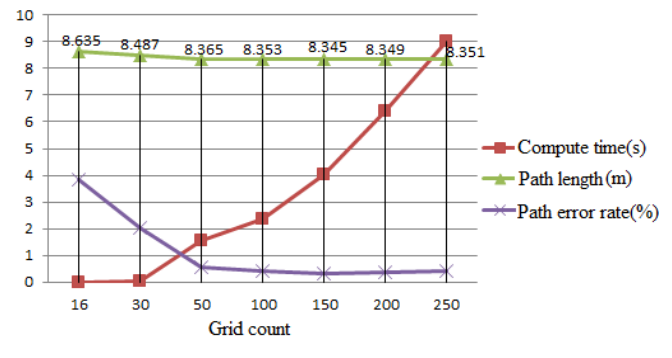
\includegraphics[width=1\textwidth]{fig/graph_grid_system.PNG}
%    \caption{Graph showing computation cost as a function of grid count~\cite{xu2017bim}}
%    \label{}
%\end{figure}

%They show what happens with the computation time when increasing the number of nodes. And also shows how minimal an effect it has on the path length.

%\begin{itemize}
%    \item Explain visibility graphs
%    \item Explain that different approaches had been used in the past, literature review, include articles.
%\end{itemize}

\begin{figure}[H]
    \centering
    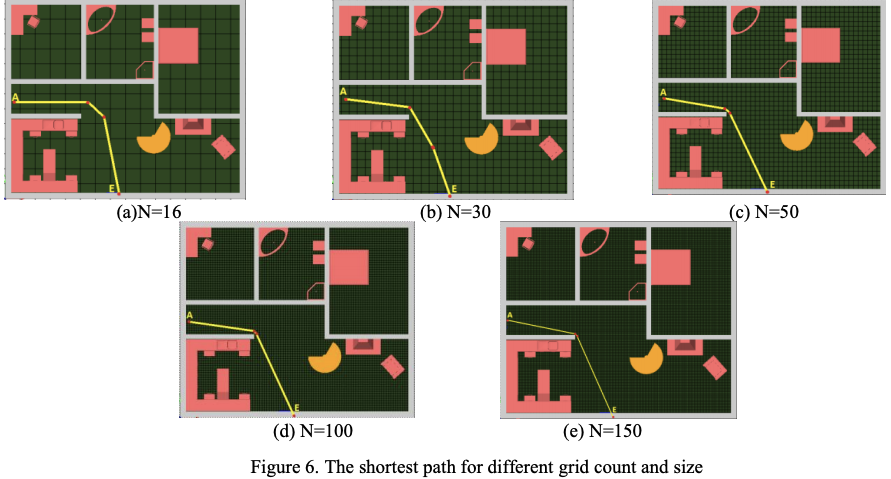
\includegraphics[width=1\textwidth]{fig/report/grid_fra_paper.png}
    \label{}
    \caption[]{Grid from paper}
\end{figure}
A paper that decided not to use the grid based system was this paper \cite{lee2010computing}. They chose a graph connectivity approach to indoor pathfinding.
\begin{figure}[H]
    \centering
    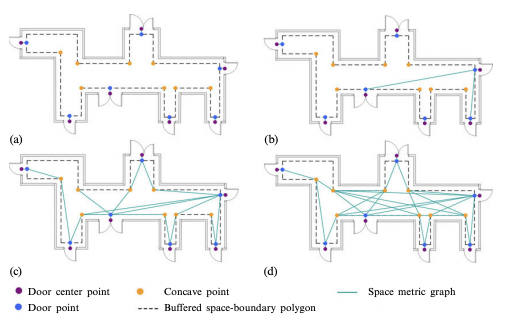
\includegraphics[width=1\textwidth]{fig/report/graph_connectivity_paper.png}
    \label{}
    \caption[]{Graph connectivity paper}
\end{figure}
The two papers illustrated that both the grid based world and the graph connectivity world were reliable approaches to take for doing path finding.

\section{Spot}
%Hvad er cad modeller og robotten.
%Giv en kontekst.
%Hvorfor er vi interesseret i at løse problemet.
The Spot robot is produced by Boston Dynamics and is their first commercially available robot currently being sold for a minimum of 74.500 dollars \cite{spot}. Spot is a quadruped that resembles a dog. It can be controlled with a tablet controller, but it can also be programmed to do autonomous tasks. This can be done using Spot's own Python SDK. The purpose of Spot is according to Boston Dynamics the following: "Spot Explorer is designed for developers eager to explore how flexible mobile robots can be adapted for tasks ranging from industrial inspection to entertainment."\cite{spot}

Industrial inspection is precisely what Spot will be used for in this project. Although this project does not work with Spot directly the project does take into consideration it's dimensions and capabilities when programming the path. The actual programming of Spot to walk the path programmed in this project, will be something for a future project. \ref{Future_work}

One of Spot's more useful properties is obstacle avoidance. Say we tell Spot to go from a point x to another point y - either by using it's controller or by a programmed path - if there is an object that blocks the straight path between point x and point y, Spot will be able to detect this object and move around it. 
This is a useful feature because it allows us to program a path for Spot without having to worry about it bumping into objects that would stand it its way such as furniture or construction tools.
Spot can also walk up and down stairs which will also be interesting for future development of this project, allowing it not only to walk around one floor but multiple floors.

\begin{itemize}
    \item Write about its length and width.
\end{itemize}

\begin{figure}[H]
    \centering
    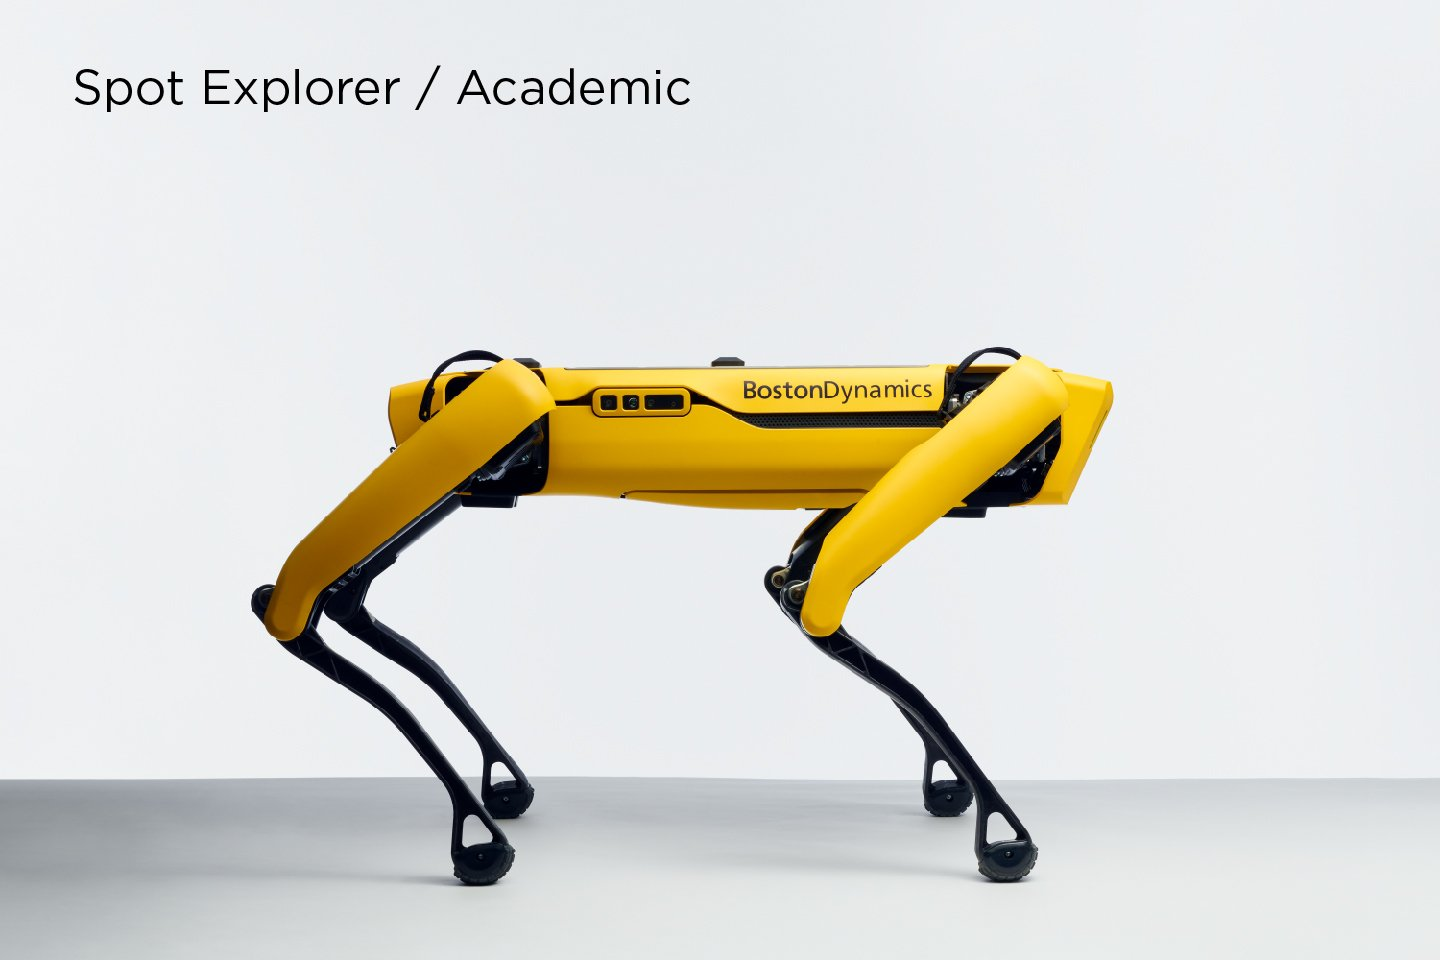
\includegraphics[width=1\textwidth]{fig/report/Spot Explorer-1.jpeg}
    \label{}
    \caption[The SPOT robot]{The Spot robot\textbf{}~\cite{spot}}
\end{figure}



\section{Data set}\label{dataset}
This project works with Building Information Modeling (BIM) data. 
The difference between Computer Aided Design (CAD) and BIM is that there is semantic information associated with each element in BIM data. In CAD a line is a line while in BIM a line can have the properties of being a wall. Not only that you can have all the parameters and properties of the wall associated with it.
\cite{bim_vs_cad}
BIM data goes beyond capturing just the geometric information, it also captures the semantic information associated with the building which allows it to better model reality. %This is why it was made mandatory in Denmark.
There are different formats for BIM data but the format of the data used in this thesis is the Industry Foundation Classes (IFC) format, which is the official international standard format for BIM models. 



\begin{comment}
In the data The coordinates are given in a polygonal triangle structure. This means that the floor plan is drawn from these coordinates by a mesh of triangle polygons. Each room from in the floor plan consists of its own tree branch, which makes it easy to include or exclude rooms in the floor plan.


The data set used in this project consists of html code of the room coordinates and the door coordinates in the format of the file is IFC (Industry Foundation Classes). [insert reference: https://fileinfo.com/extension/ifc]
[Insert picture of data]
Describing rooms and floor plans with triangle forming coordinates is a common way and makes sense for many reasons.
(Insert article reference that describes this way of plotting rooms)
(Insert picture of floor plan with triangles).
\\
The door coordinates also consists of the set of 3 coordinates with a x,y and z coordinate. Where the z coordinate says how tall the door is. 
\\
BIM models is also available for use, but will not necessarily be used since we start by modelling in 2D.
(Describe BIM models)
\begin{itemize}
    \item Write the format of the code
    \item Triangulation of the coordinates makes up the room
    \item Write about door information
\end{itemize}

Ifc is primary standard for BIM models
IFC is a schema not a format 
https://bimconnect.org/en/software/what-is-ifc/
Great interoperativebility
IFC format is compulsoary in Denmark for publicly aided building projects
IFC xml is less used for bigger buildings
object based inheritance hierachy

%In IFC open shell you it still wouldn't be a piece of cake
%probably have to take care of the triangulation on your own perhaps..
Since it is only simple version of IFC with simple objects I can use my own loader.
.
"The BIM approach is to use actual elements to represent real-world"
components.
Revit is designed for bim models.
CAD can be used for the design of everything from iphones to buildings.
BIM is a designing pattern focused for buildings only.

"Basically, when using CAD for building design, you focus on creating drawings. When using BIM, you focus on creating a building model and then the drawings can be generated from the model. "

https://knowledge.autodesk.com/support/revit-products/learn-explore/caas/video/youtube/lesson/143344-courseId-100332.html

This is the autodesk handbook on IFC format.
https://damassets.autodesk.net/content/dam/autodesk/draftr/2528/180213_IFC_Handbuch.pdf

\end{comment}






\section{Graph Theory}
As explained in the objective section \ref{Objective} of the introduction a big part of this project relies on the use of graphs, therefore graph theory plays a big role in this project. 
The program is essentially representing the building using two graphs.%, where one is a subgraph of the other. 
For the first graph the building is discretized and sampled in a grid. Each grid point is in this graph represented by a node. This will be called the "grid"-graph.
For the second graph each room of the building is represented as a node. This is called the "room"-graph.
In the following sections the relevant graph theory will be explained, which will form a basis for the Travelling salesman algorithm used to solve the path finding problem.


\subsection{What are graphs?}
Graphs are used in a wide variety of different fields to model networks and in general connections between different objects. This could for example be in electrical networks to model the relationship between resistors and capacitors or in social sciences to model connections between human beings.

A graph can be formulated as a function of nodes and edges.
$G(n,e)$
[insert picture]
A graph can be directed or undirected. With a directed graph the edge between two nodes represent a one way connection, the edge is thereby "directed" from one node to another. In an undirected graph there is no general direction meaning you can go from node a to node b and from node b to node a. In this project the program works with undirected graphs since if there is a connection between two rooms it is assumed that Spot can walk from room a to room b the same way it can walk from room b to room a, and the cost of the walk will also be identical [chapter 10 \cite{bondy1976graph}].

The edges of the graph can also be weighted or unweighted. In this project the program works with weighted edges where the weights of the edges are equal to the euclidean distance between the two nodes.



\subsection{Connectivity}
The approximate solution to the traveling salesman problem used in this program - explained further in \ref{TSP} - has a prerequisite that the graph used is fully connected - also defined as complete.  
Connectivity is a measure of how connected the nodes of the graph are. A minimal connected graph is a graph that if one of the edges is removed the graph will become disconnected. A fully connected or complete graph is a graph where every node has an edge to every other node in the graph. [insert picture of the two examples.] chapter 3 \cite{bondy1976graph}


\section{Minimum spanning tree}
Another concept needed to solve the Traveling salesman problem is the minimum spanning tree (MST). The idea behind minimum spanning tree is to find a minimal connected graph with the minimum summed edge weights. For a given graph there can be multiple minimum spanning trees since different trees can have the same minimum summed edge weights. chapter 23\cite{cormen2009introduction}

There exist different algorithms to find the minimum spanning tree of a graph. In this program the minimum spanning tree is found using the build in function in the networkx library. This function uses Kruskals algorithm to find the minimum spanning tree. chapter[23.2]\cite{cormen2009introduction}


\section{Shortest path problem} 
Before finding the minimum spanning tree another important thing to do is to find the minimum distance between two nodes in a graph. We want to find the minimum distance between all room nodes and use the distance as the weight of the edges between the nodes. This way we will have the complete "room" graph and can from there start solving for the traveling salesman problem.

There exist different shortest path algorithms. The one chosen in this project is the A star algorithm, which is an optimal algorithm, meaning it guarantees to find the shortest path. \cite{A_star} 

The A star algorithm works by using information about how far a node is from the start node and how far away it is from the end node to assess which direction to move in. When deciding on which direction to move it evaluates each neighbour cell their g(n)-cost, h(n)-cost and f(n)-cost. The g(n)-cost 
is the cost from the start node to node n, the h-cost is the cost from node n to the end node, measured with some measurement heuristic, like the euclidean distance for example. The f(n) cost is the sum of the g(n) cost and the h(n) cost. The algorithm moves to the node with the lowest f(n) cost.

[insert sketch]
%\begin{itemize}
%    \item Explain briefly how it works.
%\end{itemize}
%Again the Networkx framework has a built in function for the A star algorithm.





\section{Spatial Data structures}
Spatial data structures are data structures that store objects and the geometric information associated with the object. The objects are stored at the leaf nodes of a tree-structure where the branches of the tree indicate separation in space. chapter 1. \cite{laurini1992fundamentals}. [insert figure] %The searching algorithm used in this project is the nearest neighbour algorithm.
The main use of spatial data structures in this project is to quickly find the nearest objects to a given node. This could for example be to find the closest wall to a given node. Having a data structure that allows for fast access to nearby objects can drastically speed up the program, since the alternative method would be a brute force approach where each object would have to be checked to find the nearest object.


There exist different spatial data structures but most of these work only with point objects. This is for example the case with  KD-tree, which is a binary tree that for every branch splits space in two and has point objects at the leaf nodes. \cite{bentley1975binarysearch}. 

In this project we are interested in storing multidimensional objects - such as walls and rooms - as well as point objects and we are therefore interested in using a spatial data structure that allows for storage of such multidimensional objects.

One spatial data structure that meets these criteria is the R-tree.

%\begin{itemize}
    %\item Explain more about spatial data structures and their uses especially in graphics.
%\end{itemize}

\section{R-tree}
R-tree is an abbreviation for rectangle tree which is a suitable name since it works by making a bounding box - bounding volume in 3D - around the objects in a hierarchical structure. \cite{guttman1984r}. When a query is made the R-tree checks which of the bounding boxes at the top layer intersects with the bounding box of that query, and then goes a level deeper on the branch of the bounding box it intersected with. I keeps doing this until it hits the leaf nodes or until the bounding box of the query does not intersect with any of the rectangles in the given layer.
 
To illustrate how this hierarchical structure works take for example the  elements in a house. At the top level we have the house itself. Inside the house we have different rooms, each of which can be bounded by a box. Inside each of the rooms we have the furniture which can also be bounded by a box. When a query is made the R-tree first checks if the query intersects with the bounding box of the house. If this is the case it checks which of the rooms it intersects with and so on. In this way the R-tree returns the objects that are closest to the query. 




%\section{Grid data vs visibility graph}
%To make the robot walk from one room to another or one place in the building to another, it is important to understand  and decide on a way to implement the connectivity between the rooms. There are mainly two different kinds of implementations; a graph connectivity implementation and a grid implementation.

%The grid implementation works by discretizing the floor of the building into a grid with nodes of a specific size; the smaller the node size the higher the resolution of the grid.

%The graph connectivity approach works by representing each room/area by a node/dot which will be connected by a line to other rooms in the floor.

%The different implementations have different advantages and limitations. For example computationally the graph connectivity approach is much more scalable with bigger buildings or construction sites where as implementing a grid system in these situations will be more taxing computationally since a lot of nodes will have to be calculated. 

%On the other hand the advantage of the grid method is that its pathfinding algorithms will work on all building shapes. 
%Imagine the floor plan of the building below:


%\begin{figure}[H]
%    \centering
%    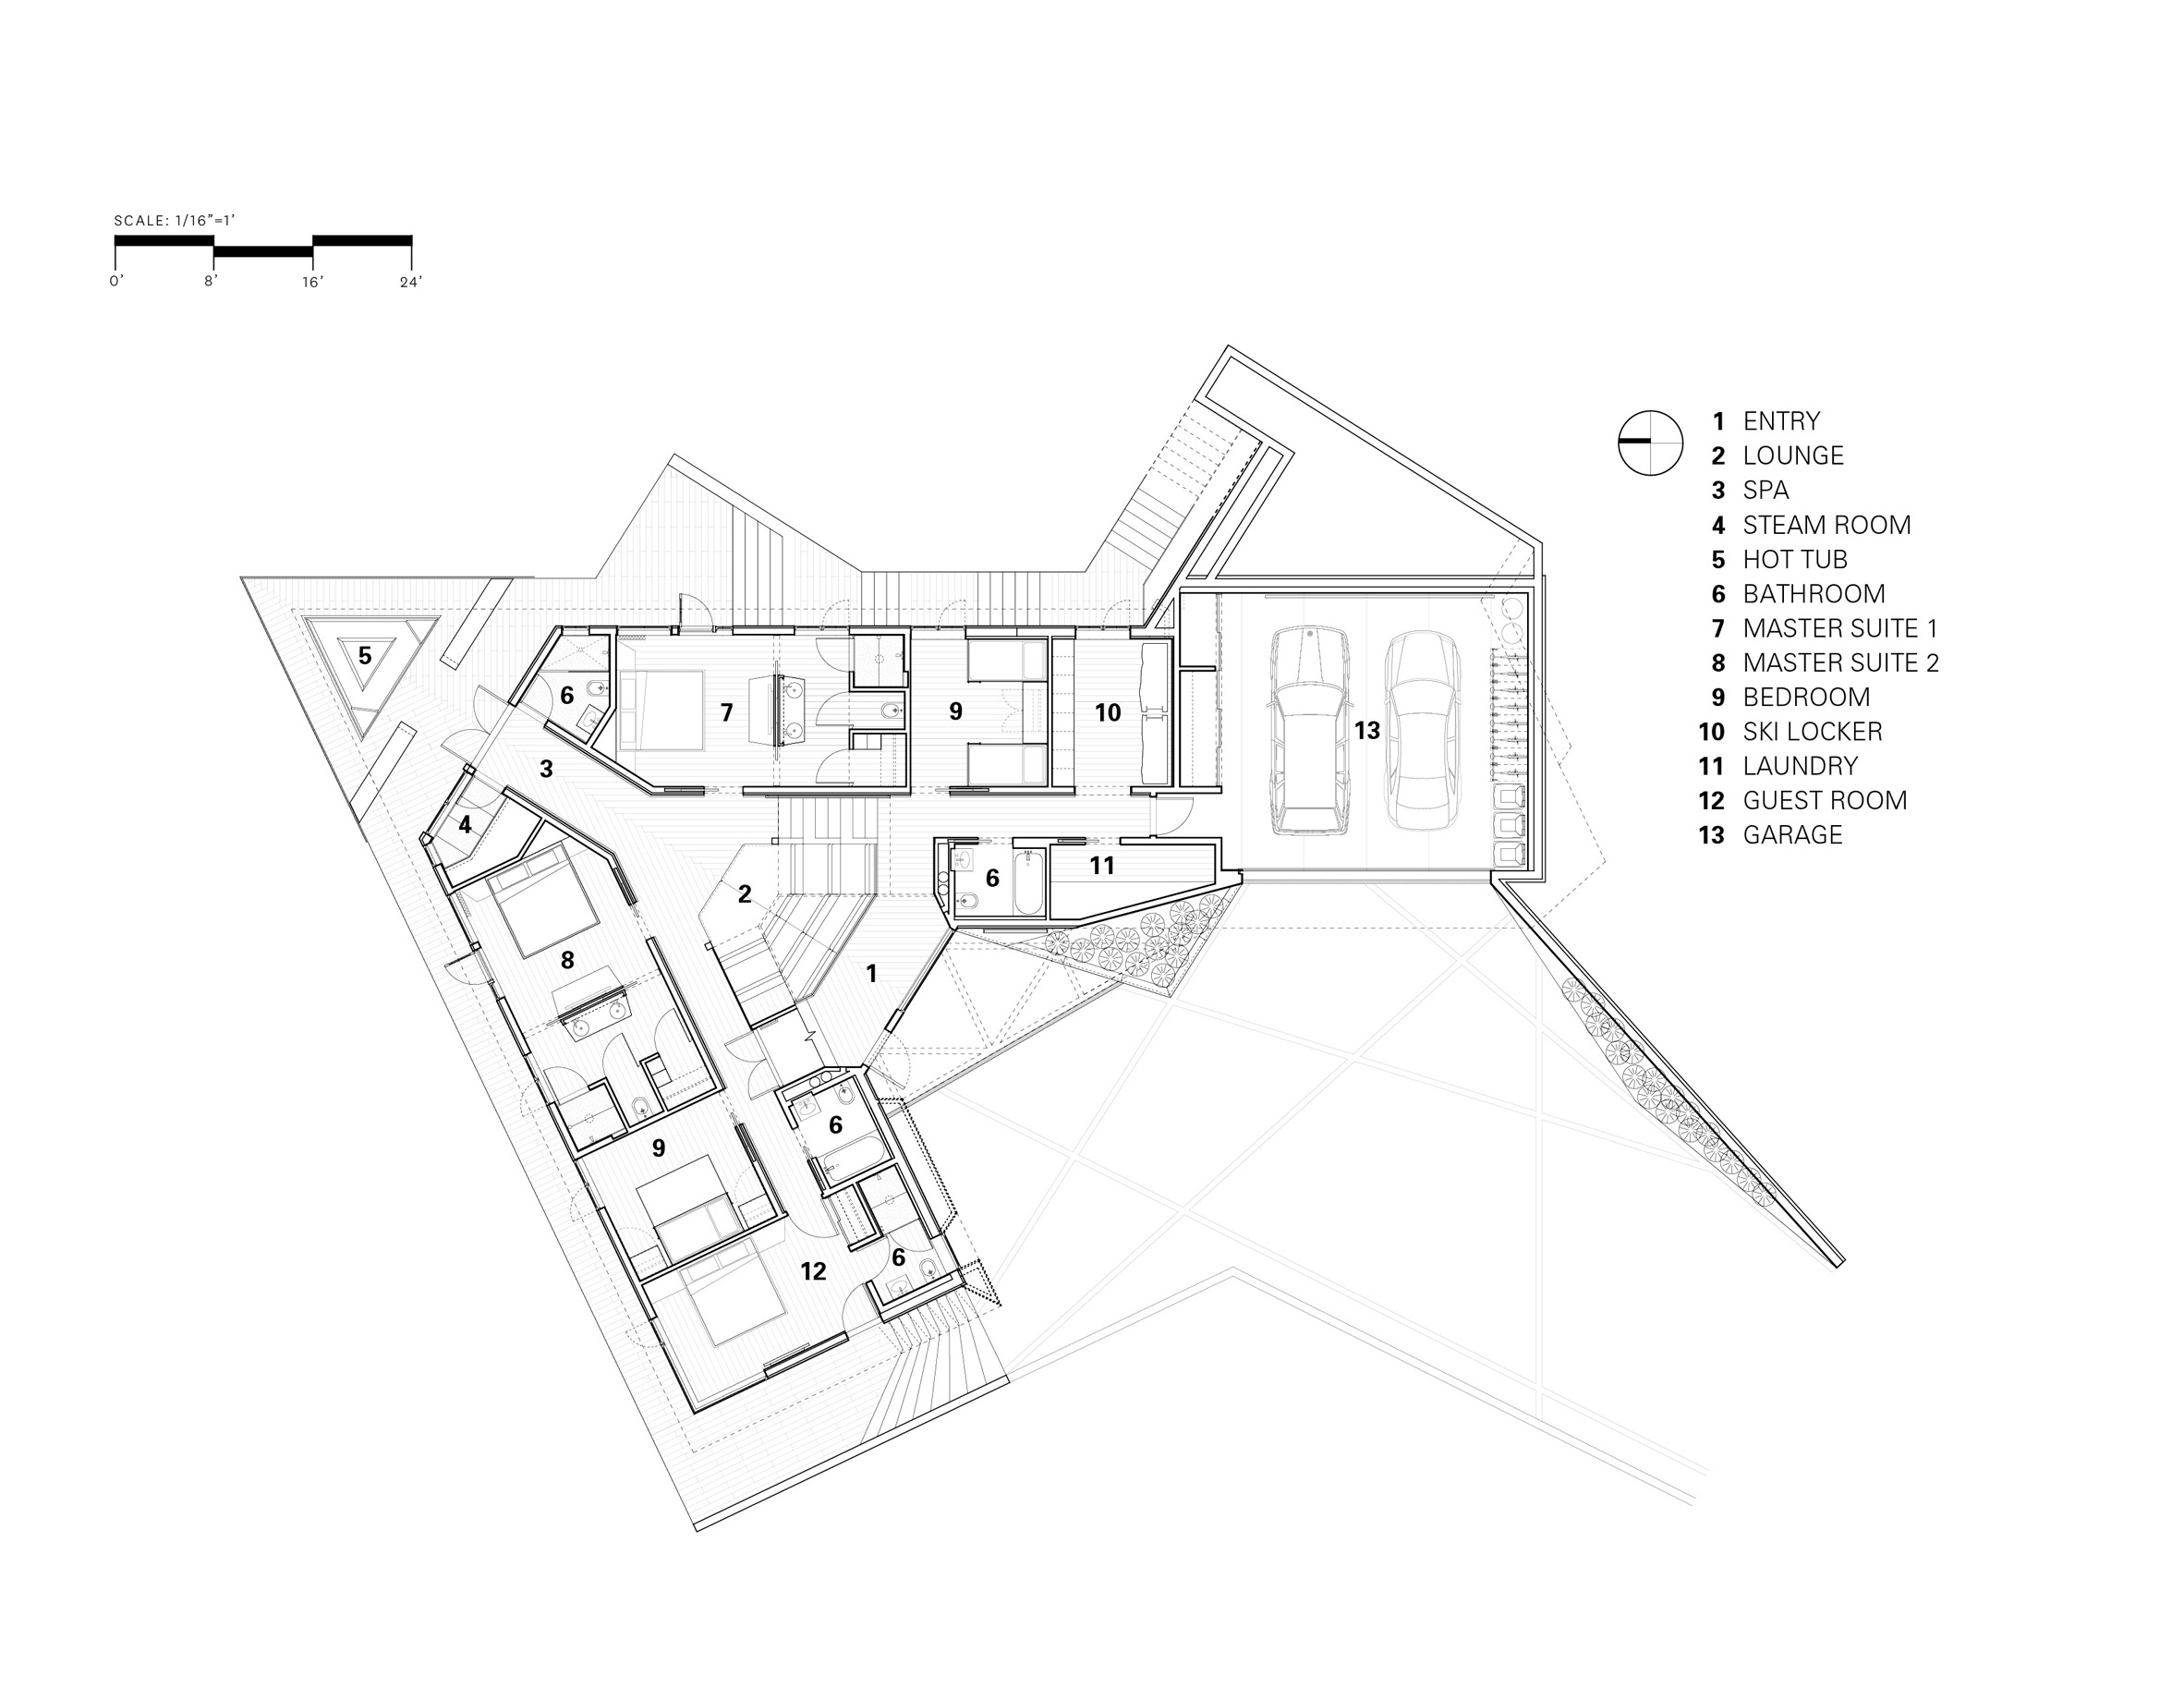
\includegraphics[width=1\textwidth]{fig/weird_floorplan.png}
%    \label{}
%    \caption[Weird floor plan]{Weird floor plan~\cite{weird_building}}
%\end{figure}

%When using a grid system apporach it will be possible to get an agent to walk from area 12 to 13 by specifically telling it which nodes are walkable and which nodes are not e.g walls. This will not be possible for the graph connectivity graph. The graph will here see only that area 12 and 13 are connected but not in which way. The method will draw a straight line between the two points and not see that the areas in reality are connected by the long pathway that goes through the entire floor plan.





\section{Distance field}
Which nodes in the building that Spot can traverse and which it can not traverse is determined with the use of distance fields. 
The distance field works with a grid based graph systems. There are different variations of the distance field \cite{distance_field} but the one used in this program is a distance field where each node in the grid is associated with an attribute that indicates the euclidean distance to the nearest wall. This attribute is then used to remove nodes that are too close to their nearest wall allowing for a realistic buffer space between Spot and the walls of the building. This is also known as a Boolean distance field.


%When humans walk around in a building we don't walk right next to the wall, scraping our shoulder to the wall (unless the path is very narrow) the same should be the case for the robot. If there was no buffer zone in front of the walls of the building, one could imagine that when Spot would have to turn a corner the program would tell it to walk right alongside the wall since this would allow for the shortest path to turn the corner.

%Making use of the distance field is the entire reason the grid structure of the graph was chosen over the visibility graph structure.

%The distance field allows for certain advantages that makes it a very robust solution. It is a robust solution because it for all nodes in the grid indicates whether Spot can traverse the node or not. This makes the approach useful for all kinds of obscure buildings.  


\section{Ray casting algorithm}
Figuring out which room each node in the grid belongs to is an important step before generating the room nodes and is based upon the usage of the ray casting algorithm.
This algorithm checks whether a point is inside a polygon or outside a polygon. 
It works by casting a ray in a random direction from the position of the point towards infinity. It then counts the number of times the ray intersects with a line. If the ray intersects an even number of times with the lines of the polygon it means the point is outside the polygon, and if it intersects an uneven number of times it means that the point is inside the polygon. [insert figure] [insert reference]

To use the ray casting algorithm another algorithm is needed to check for line intersection. The details about the line intersection algorithm used in this program can be found here \cite{line_intersection}. 





\section{K-means}
The K-means algorithm is a clustering method and is used to generate the room nodes that will used as nodes in the TSP solution.
It works by first placing random centroids in the room. The number of centroids is in this case chosen as a percentage of the number of nodes existing in the room.  The algorithm then consists of two recursive parts. 
First step in this recursion is that all the nodes in the room are associated to one of the centroids depending on which centroid they are closer to.
Second step is to re-centralize the centroids so they are in the center of all the nodes associated to it. 
These two steps are repeated either a pregiven amount of time or until convergence within a $\sigma$ of the coordinates of the centroid occur. chapter 22.2 \cite{shalev2014understanding}


\section{Traveling salesman problem}\label{TSP}
The Traveling salesman problem abbreviated TSP, is one of the most well known optimization problems. The problem was first defined in the 1930's by the mathematician Karl Menger, who presented it as the "messenger" problem. page 41 \cite{schrijver2005history} 
The original idea behind TSP is to solve the challenge of a salesperson having to visit a certain number of cities, the person is only allowed to visit every city once except the starting city which will also be the end city. This is also known as a Hamiltonian cycle. The challenge is now to optimize for the distance travelled, such that the overall distance for the entire route is minimized. chapter 35.2 \cite{cormen2009introduction}
The TSP optimization problem is a NP-hard problem which means it can not be solved in polynomial time but only in exponential time. This means that for non trivial cases of TSP approximate solutions are needed. 

Since the idea of this program is for it to work on many different buildings with various sizes, the number of nodes needed to be visited can vary a lot. Using an approximate algorithm to solve TSP was therefore considered a better option than trying to find an optimal solution to the problem. 
Furthermore robustness of the program was considered a higher priority than finding an optimal route for the robot to traverse. See \ref{setting_prioritie}
In this project we work with the metric TSP problem. In the metric TSP problem the triangle inequality holds, which says that the direct path between two nodes a and b is always equal or shorter than the path that includes and intermediary node c. 



%Explaining the different optimal solutions of this problem is beyond the scope of this report.

%\section{approximate solution}
%Different approximate solution algorithms exist for TSP. A few parameters play a role when choosing which algorithm to go with. One parameter is how is the time performance, meaning how long will it take the program to run this algorithm. Another is how close to the optimal path will the solution be. The third thing to consider is how easy is the algorithm to implement given the frameworks and tools available to us.
%Neither time nor performance are important factors in this program. Instead of spending a lot of time in analysis of the different algorithms and their theoretical constraints and performances the algorithm chosen in the end was chosen with ease of implementation in mind. The 2-opt algorithm was chosen.
%\begin{itemize}
%    \item There are a lot of different approaches ant colony, nearest neighbour, christofides, 2-opt algorithm and others. The one went with was the 2-opt. Important that they run in polynomial time. The 2 opt is at most twice the optimal length while christofides is 1.5 optimal length, the 2 opt has shown to be around 5 \% better. Both could have been chosen, in this case I chose the 2-opt algorithm
%\end{itemize}

\section{2-opt algorithm}
The 2-opt algorithm is an approximation algorithm to solve the traveling salesman problem. The name of the algorithm stems from the fact that the cost is at most 2 times the cost of the optimal path. 
The algorithm consists of 4 parts. First a complete graph is needed. Second a minimum spanning tree for the graph is generated. Third a depth first traversal is performed. Fourth duplicate vertices are removed from the tree.
This gives an approximate solution to TSP that is at most 2 times the cost of the optimal path for the graph. Kap[35.2.1] i \cite{cormen2009introduction}

Depth first search traversal is a concept in graph theory, where a branch in a graph-tree is searched first before searching other branches. The search goes deeper until it finds the end node of the branch. This is opposed to breadth-first search where it searches the one level of the graph-tree before searching the next level.Kap[22.3] \cite{cormen2009introduction}



%\begin{itemize}
%    \item Explain depth first search traversal
    %\item Explain Hamiltonian cycle
%\end{itemize}






















%-----------------------------------------------%
\begin{comment}
\section{Grid vs polygonal}
\subsection{Unity vs python}
The problem with unity was that it was difficult to import floor plans in a good way.

Talk about how you could use the grid version or the polygonal version. Spent a good amount of effort here.

\section{Which platform to use}
\begin{itemize}
    \item Write about which platform to use. The pros and cons of each. Ros vs Unity vs Python.
\end{itemize}



\section{Dijkstra's algorithm}
Dijkstra's algorithm is an algorithm to find the shortest path between two nodes in graph. The way it works is by first having a source node or initial node. The distances to all other nodes will be initialized to infinity since the distances are unknown for now. Then the algorithm will look at the neighbour nodes of the source node. It will evaluate the distance to each of the nodes. The distances of the nodes will then be updated in the table of distances, since it is no longer infinity. With done the start node has been visited and will no longer be visited. The next node in the algorithm to evaluate will be the node with the shortest distance to the start node. The neighbours to this node will now be evaluated and again the distance table will be updated. This pattern will keep repeating until all nodes have been evaluated. 

\section{A*}
A

\section{How to get around the building}
The way to get around the building is using visibility graph. Here you make a node on each portruding corner and also on the doors. This way a path between all nodes can be constructed, this is called a visibility graph.
(reference the master thesis).

\subsection{Convex decomposition}
In the report written by nikolaj and co. The way they solved the general pathfinding problem through the building was using Convex Decomposition. The idea in convex decomposition is to split non convex polygons - in this case the polygons represent the rooms of the floor - into convex subparts. Each convex subroom will then be assigned a node. A room is non convex if a corner of the room has an angle of more than 180 degrees. In these cases we get scenarious where 2 nodes in the same room are not necessarily connected by a straight path [insert sketch]. A convex room on the other hand has no corners of more than 180 degrees and therefore ensures that any 2 nodes in room is connected by a straight path. 
When a room is divided into its convex subparts a node is placed in the intersection of these two rooms and connection is thereby ensured between all areas in the original room.
Doing this convex decomposition of the rooms therefore makes the use of corner nodes superfluous since role of the corner nodes was to make this connection between the different areas of the non convex rooms.

Convex decomposition has a limitation when it comes to obstacles - that are visible from the graph i.e pillars - it has no good way to deal with these. This is the same with the portruding corner node approach. Neither of these two have good ways to deal with obstacles or narrow paths.

\subsection{The challenge of obstacles}
What to do with these obstacles like pillars.


\section{How to get from room to room/around the building in an appropriate way?}
Do we want the shortest route?
Do we want the route










\section{Dimensions of robot/ collision detection}
\begin{itemize}
    \item Write about how to incorporate the dimensions of the robot in your simulation
\end{itemize}


\subsection{Distance field vs distance route}
The dimensions of the robot is mostly needed to make sure that the robot does not bump into walls or other objects. And also to make sure that a path that is deemed traversable is not in reality too narrow for the robot to pass through.
So far the robot has been modeled by a point, it is now time to include a radius to that point which will represent the robots dimensions.

There are mainly 3 concerns for the robot when it wants to traverse the floorplan now. One is the concern of too narrow paths. The other is the concern of obstacles that are seen from the floorplan i.e pillars. And the third are obstacles not seen from the floorplan, maybe a chair or a table etc.



There are multiple ways to go about the challenge of incorporating the dimensions of the robot in the simulation. 
One way is to discretize the entire map and for each cell find the distance to the nearest wall. If the distance from the wall to the cell is smaller than the radius of the robot, the cell will be deemed not traversable since this means that the robot will hit the wall. If the distance to the wall is larger than the radius the cell is traversable. What we get by doing this is a boolean distance field. Where we have nodes that are traversable and nodes that aren't.
The issue with this approach is that it is not very scalable to bigger buildings. More on this is written in chapter 10.
The good thing about this approach is that it is easy and a straightforward way to tell the robot which places it is allowed to traverse and which are not. It can not go wrong with this approach. 
It is also fast to look up because you have done the preprocessing before hand.
Another pro of this approach is that it will be beneficial when we later want to find optimal node placements in the rooms we are visiting.

The other way is to discretize the route. This is a bit more complicated implementation but will be rewarded by its scalability to bigger buildings. 
The idea here is to only discretize the route that the robot will walk instead of discretizing the entire map. 
Along the route  the robot will check if it is near a wall using a distance function. The interval here can be dynamic e.g if the distance to the nearest wall is 5 meters and the radius of the robot is 1 meter it can walk for 4 meter without hitting a wall.
This means that between 2 nodes - a start and an end node - a lot more nodes will be placed. The robot will go to a node find the distance to the nearest wall and then check walk in a straight line towards the node it is seeking the same amount as the distance to the nearest wall minus the radius. Then it will check again to see what the distance to the nearest wall is and repeat the process. It is important that the room/end nodes are a certain radius away from the walls to begin with. 

One way to go about this is to check the distance to all the walls for every node. This does not scale very well when the number of walls increases. 
Another way is to have a certain datastructure that takes all the walls and find the nearest quickly.

One other problem with discretizing the route is that a large percentage of the time the obstacle between 2 room nodes are walls and this means that this A star algoritm will often fail, since the only way to walk through walls are using the doors. 

A third way is to follow the same scheme as has been done so far and only rely on corner nodes and door nodes to go from node to node. This should in theory work and should only not work when we have a straight path that is too narrow. In these cases which will be very rare what will happen is that the robot wont be able to walk through it and we will tell it that it should do the tsp solution again and make the connection between these two nodes not traversable.



So how is convex decomposition related to the dimensions of the robot? Well doing convex decomposition by itself does not ensure that all nodes placed on the floorplan are in accordance with the requirements needed to allow for the dimension of the robot. This technique would have to be combined with a distance measure to the nearest wall being larger than the radius of the robot.


\subsection{Random placements of nodes}
I will have to think about this mehtod.
In this method the idea

\subsection{A star discrete route}
This is the second argument in this area.


\section{Data structure for the walls}
Explain the purpose of space partitioning algorithms

\subsection{Binary space partitioning}
Binary space partitioning trees is a datastructure used to partition polygons in space. One of its big uses are in computer graphics where it is used as a solution to the issue of Visual surface determination. [insert reference: https://twobithistory.org/2019/11/06/doom-bsp.html]
The renderer of a computer game has to figure out which objects can be seen and not seen from the vievpoint of the player.

Compared to raytracing which is an image first renderer BSP is an object first renderer. This means that rather than tracing each pixel in an image like raytracing does, BSP traces each object in the scene and is therefore more cost effective.

BSP trees are useful when wanting to display the viewpoint of an agent. Since it splits the areas in lines such that there are polygons behind and in front of each line. This is not really what we are looking for in this project. For us i doesn't matter whether the closest wall is directy in front of the robot or directly behind it since this doesn't influence whether it will hit the wall. Or maybe it is only necessary to look at walls straight ahead of you?

BSP is used in collision detecting in robotics. [ref: https://www.wikiwand.com/en/Binary_space_partitioning]
A disadvantage of binary space partitioning is that generating a BSP tree can be time-consuming.Typically, it is therefore performed once on static geometry, as a pre-calculation step, prior to rendering or other realtime operations on a scene. It is an expensive pre process. 

It may not be useful here since we are not working on real time applications.





\subsection{KDtrees}
Hvorfor du vælger kd TRees i forhold til BSP trees.
The idea here is to cut the space into halves.
binary search tree with multiple values.
Still a logarithm search in terms of number of nodes in the tree.
You pick a random dimension.
You find the median.
You split the data. 
Pick another dimension. etc.

Usefull algorithm to find nearest neighbour.


The idea behind this structure is to take the center point of each line and partition it into 1 of 4 or 16 corners. Lets start with 4 for simplicity. For each line center we check if its x value is larger or smaller than the grid center x value. If it is larger this means that it will be placed on the right hand side of the map. We then check the y value and do the same. IF it is larger than the center y we place it on the upper part of the map and if it is smaller we place it in the lower part of the map. We have now partitioned the walls into one of 4 sections. We can partion it further if we wish so. A more stable approach is to take each of the points that the line consists of and do the partioning for each point. In this case the line can be part of multiple areas of the map. This is more stable since we can have scenarious of big walls that strectch multiple areas of the map and the grid point could be very close to one of the edge points of the line but not very close to the center of the line.
For each grid point we then check where in the map it is partioned. 

A scenario where this algorithm could fail is when it is close on the edge between two adjacent areas. In this case there could be a scenario where it is closer to a wall on the adjacent area than any of the walls in the area that it is in.
This can be made a non issue by making sure that the point is not less than the radius of the robot away from the intersection between the two areas. If this is the case it doesn't matter if it is closer to a wall on an adjacent area because it will still conform to the dimensions of the robot. 



















\section{Optimal placement of nodes}
\begin{itemize}
    \item Write about scenic route vs discrete points.
    \item Write about SLAM
    \item optimal placement of nodes
\end{itemize}

\subsection{Simultanous location and mapping}
As the name indicates SLAM is about localizing your robot in the map while you also do the mapping part. The way this is done is by using sensors such as a lidar - it could also be other types of sensors. Then there are some other steps in the process. Since inn this case the mapping has already been done it doesn't really make sense to do the SLAM. It might be a good idea to find a way for the robot to localize itself, without need to do the mapping.




\subsection{ROS}
ROS had a pretty smart technique of importing floorplans

\subsection{Python API}



\section{Future work}
\begin{itemize}
    \item A section about stairs
\end{itemize}

\end{comment}

\chapter{Design}
%\section{Design overview}
% Consider making this a chapter of its own
\section{How the three step plan got formulated}
It became obvious from the beginning of this project that there were different ways to go about solving this path finding problem. One of the first realizations that arose was the similarity of this problem with the traveling salesman problem. Both problems were about visiting certain number of nodes before returning to the start node; in the travelings salesman problem the nodes represent cities and in this problem the nodes represent rooms. This would serve as the starting point of the thesis. The question would later be how to go about representing the places that the robot had to visit. An obvious solution was to have a graph where the nodes represent rooms and the edges would represent the connection to those rooms [insert picture of simple graph].

\begin{figure}[H]
    \centering
    \includegraphics[width=1\textwidth]{fig/report/tilhørende_tsp_solution.png}
    \label{}
    \caption[Design overview]{}
\end{figure}

This simple representation would have a few challenges associated with it, the main one being that a straight line between two room nodes would not model very well the real connection between the two rooms. Spot would not be able to walk in a straight line from one room to another because there would be walls blocking the path. 
The graph therefore needed to have a little more information, so door nodes and corner nodes were added. The door nodes would be the only nodes that could cross walls. The job of the corner nodes would be to act as a concave point i.e a point that would be placed at 90 degree or more corners. With this information the first basic solution to the problem could be made. [insert basic solution to the problem].
\begin{figure}[H]
    \centering
    \includegraphics[width=1\textwidth]{fig/report/tsp_solution_med_mange_døre.png}
    \label{}
    \caption[Design overview]{}
\end{figure}

The issue now was to account for the dimensions of the robot in the graph. So far it would only be represented as a point with radius 0. Accounting for the dimensions would show itself to be one of the main challenges of this project. 
The same way that when people walk around in a building they don't walk right next to the wall, scraping their shoulder to the wall (unless the path is very narrow) the same should be the case for the robot. If there was no buffer zone in front of the walls of the building, one could imagine that when Spot would have to turn a corner the program would tell it to walk right alongside the wall since this would allow for the shortest path to turn the corner.


It became clear that some form of discretization would have to take place to indicate exactly where Spot could be and where it could not be.
The question was whether to discretize the entire map or discretize just the route.
% Analysis
%\section{Grid data vs visibility graph}
%To make the robot walk from one room to another or one place in the building to another, it is important to understand  and decide on a way to implement the connectivity between the rooms. There are mainly two different kinds of implementations; a graph connectivity implementation and a grid implementation.
%\\\\
%The grid implementation works by discretizing the floor of the building into a grid with nodes of a specific size; the smaller the node size the higher the resolution of the grid.
%\\
%The graph connectivity approach works by representing each room/area by a node/dot which will be connected by a line to other rooms in the floor.

%The different implementations have different advantages and limitations. For example computationally the graph connectivity approach is much more scalable with bigger buildings or construction sites where as implementing a grid system in these situations will be more taxing computationally since a lot of nodes will have to be calculated. 

%On the other hand the advantage of the grid method is that its pathfinding algorithms will work on all building shapes. 
%Imagine the floor plan of the building below:


%When using a grid system apporach it will be possible to get an agent to walk from area 12 to 13 by specifically telling it which nodes are walkable and which nodes are not e.g walls. This will not be possible for the graph connectivity graph. The graph will here see only that area 12 and 13 are connected but not in which way. The method will draw a straight line between the two points and not see that the areas in reality are connected by the long pathway that goes through the entire floor plan.
% End Analysis

\subsection{Map disretization / distance field}
One way to solve this challenge is to discretize the entire map and for each cell find the distance to the nearest wall. If the distance from the wall to the cell is smaller than the radius of the robot, the cell will be deemed not traversable since this means that the robot will hit the wall. If the distance to the wall is larger than the radius the cell is traversable. What we get by doing this is a Boolean distance field. Where we have nodes that are traversable and nodes that are not.

  

\begin{figure}[H]
    \centering
    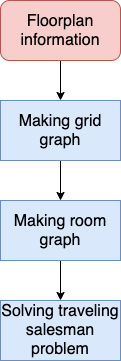
\includegraphics[width=0.4\textwidth]{fig/report/big_structure.png}
    \label{}
    \caption[Design overview]{}
\end{figure}

The issue with this approach is that the number of nodes is directly proportional to the size of the building. For bigger buildings this might cause a problem with performance of the program. 
With that said the distance field allows for certain advantages that makes it a very robust solution. It is a robust solution because it for all nodes in the grid indicates whether Spot can traverse the node or not. This makes the approach useful for all kinds of obscure buildings.
%The advantage of this approach is that it is easy and a straightforward way to tell the robot which nodes it is allowed to traverse which it can not. %This  
%It is also fast to look up because you have done the preprocessing before hand.
Another pro of this approach is that it will be beneficial when we later want to find optimal node placements in the rooms we are visiting. This is because the rooms will already be discretized which makes generating room nodes a simpler process.


\subsection{Route discretization}
Another way to go about the problem would be to discretize the route. The implementation of this would be a bit more complicated but would be rewarded by its scalability to bigger buildings. 
The idea here is to only discretize the route that the robot will walk instead of discretizing the entire map. 
%This could be done in different ways.
One heuristic to this could be that along the route Spot will check if it is near a wall using a distance function. The interval here can be dynamic e.g if the distance to the nearest wall is 5 meters and the radius of the robot is 1 meter it can walk for 4 meter without hitting a wall.
This means that between two nodes - a start and an end node - a lot more nodes will be placed. The robot will go to a node find the distance to the nearest wall and then walk in a straight line towards the node it is seeking the same amount as the distance to the nearest wall minus the radius. Then it will check again to see what the distance to the nearest wall is and repeat the process. It is important that the room/end nodes are a certain radius away from the walls to begin with. 

%One way to go about this is to check the distance to all the walls for every node. This does not scale very well when the number of walls increases. 
%Another way is to have a certain datastructure that takes all the walls and find the nearest quickly.

%One other problem with discretizing the route is that a large percentage of the time the obstacle between 2 room nodes are walls and this means that this A star algorithm will often fail, since the only way to walk through walls are using the doors. 
\\\\
In the end discretization of the entire map was chosen with the thought in mind that the program is not in real-time and therefore fast performance is not a requirement. Implementation wise the distance field would also be a more robust solution and easier to implement. With the route discretization a lot of different worst case scenarios would have to be accounted for and considered, while this would not be the case with the distance field since the program tells Spot very precisely which nodes it can traverse and which it can not. The distance field might also be a better implementation long term since it can allow for certain algorithms when placing the room nodes, explained further in \ref{k_means}.  
\\\\
Representing the building with a graph that would both allow for paths that would not traverse through walls and also allow for the dimensions of Spot, was only one part of the program. Now we would have to figure out how to solve the traveling salesman problem from there.

Looking at the approximate solutions for the TSP the minimum spanning tree of a complete graph was needed. 
Therefore what needed to be done was to make a complete graph that only consisted of the room nodes i.e the nodes that would have to be visited.  
When having that the TSP solution for the "room" graph could be found and that could be translated to the grid graph.
\\
Looking at the flowchart below this overall structure is seen. We first start by making the grid graph, that allows for legal paths and allows for the dimension of the robot. From that graph the program then constructs a room graph that is complete i.e there is an edge between all the room nodes. At last the program solves the approximate TSP for the building.

\begin{figure}[H]
    \centering
    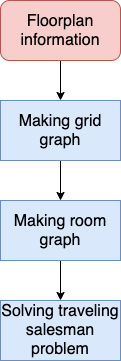
\includegraphics[width=0.4\textwidth]{fig/report/big_structure.png}
    \label{}
    \caption[Design overview]{}
\end{figure}




\section{Making the grid graph}
Looking at the figure below the flowchart of how the grid graph is generated is given. Making the grid graph we would need to sample the building with a given resolution and place a node on each sample and connecting nodes that are next to each other and diagonal to each other with edges. We would end up with a very dense and big graph. The usefulness of the grid graph is that it can have nodes that Spot can traverse and nodes that it can not traverse. Essentially the non traversable nodes are the ones near the walls - the nodes outside the building is also removed later in the program. Therefore a buffer zone between the walls of the building and the open space area is desired. We therefore need to remove the nodes that are within a certain distance of the nearest wall. For that reason the spatial data structure is made for the lines, such that the distance for each node to the closest line can be evaluated. The spatial data structure for the rooms are also made and the same for the nodes. The data structure for the rooms will become useful when making the room graph and so will the data structure for the nodes.

\begin{figure}[H]
    \centering
    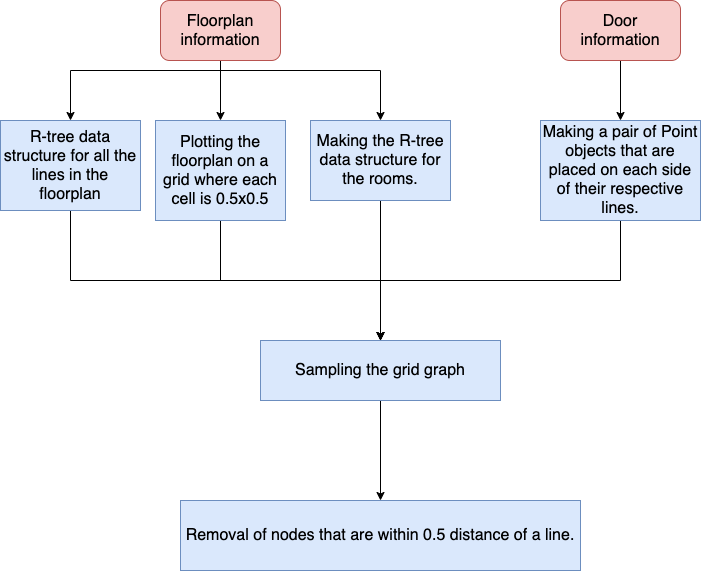
\includegraphics[width=1\textwidth]{fig/report/making_grid_graph.png}
    \label{}
    \caption[Design overview]{}
\end{figure}


\section{Making the room graph}
As explained before, after having made the grid graph, the program needs to make the room graph that needs to be complete. This is because we want to have a graph that only consists of the room nodes such that we can get an approximate TSP solution on that graph. The reason it needs to be complete is that Spot needs to be able to visit each room node from each other room node. This is needed to find the approximate solution of the TSP problem. If there are room nodes that for one reason or another can not be connected to the rest of the room nodes, they are removed from the graph, since this mean that they can not be visited by Spot.

To make the room graph the program needs to first generate the room nodes. Before the program can do that it needs to figure out which rooms each node belongs to, since it is not possible to generate nodes in all rooms with certainty if the program can not distinguish between the rooms. Therefore it first does the room labeling heuristic, which makes use of the ray casting algorithm. This is also where outside nodes are removed from the graph, since they are not part of any room.

When each node has been successfully labeled with a room number, it is time to generate the room nodes. Generating the room nodes were also one of the big discussion points of the project with a few alternative solutions available.
% From Analysis 
\section{Optimal placement of nodes}
The program needs a way to figure out where to place the "room" nodes. Ideally we want to have the "room" nodes placed in such a way that the robot can do point scans of the entire room. Different approaches can be taken to solve this challenge. 

The simplest idea would be to make a bounding rectangle of the room and place a node in the middle of that room. This would work on a lot of rooms that are already square shaped but there would be a risk of a node being placed outside the room for non convex shaped rooms. 
\begin{figure}[H]
    \centering
    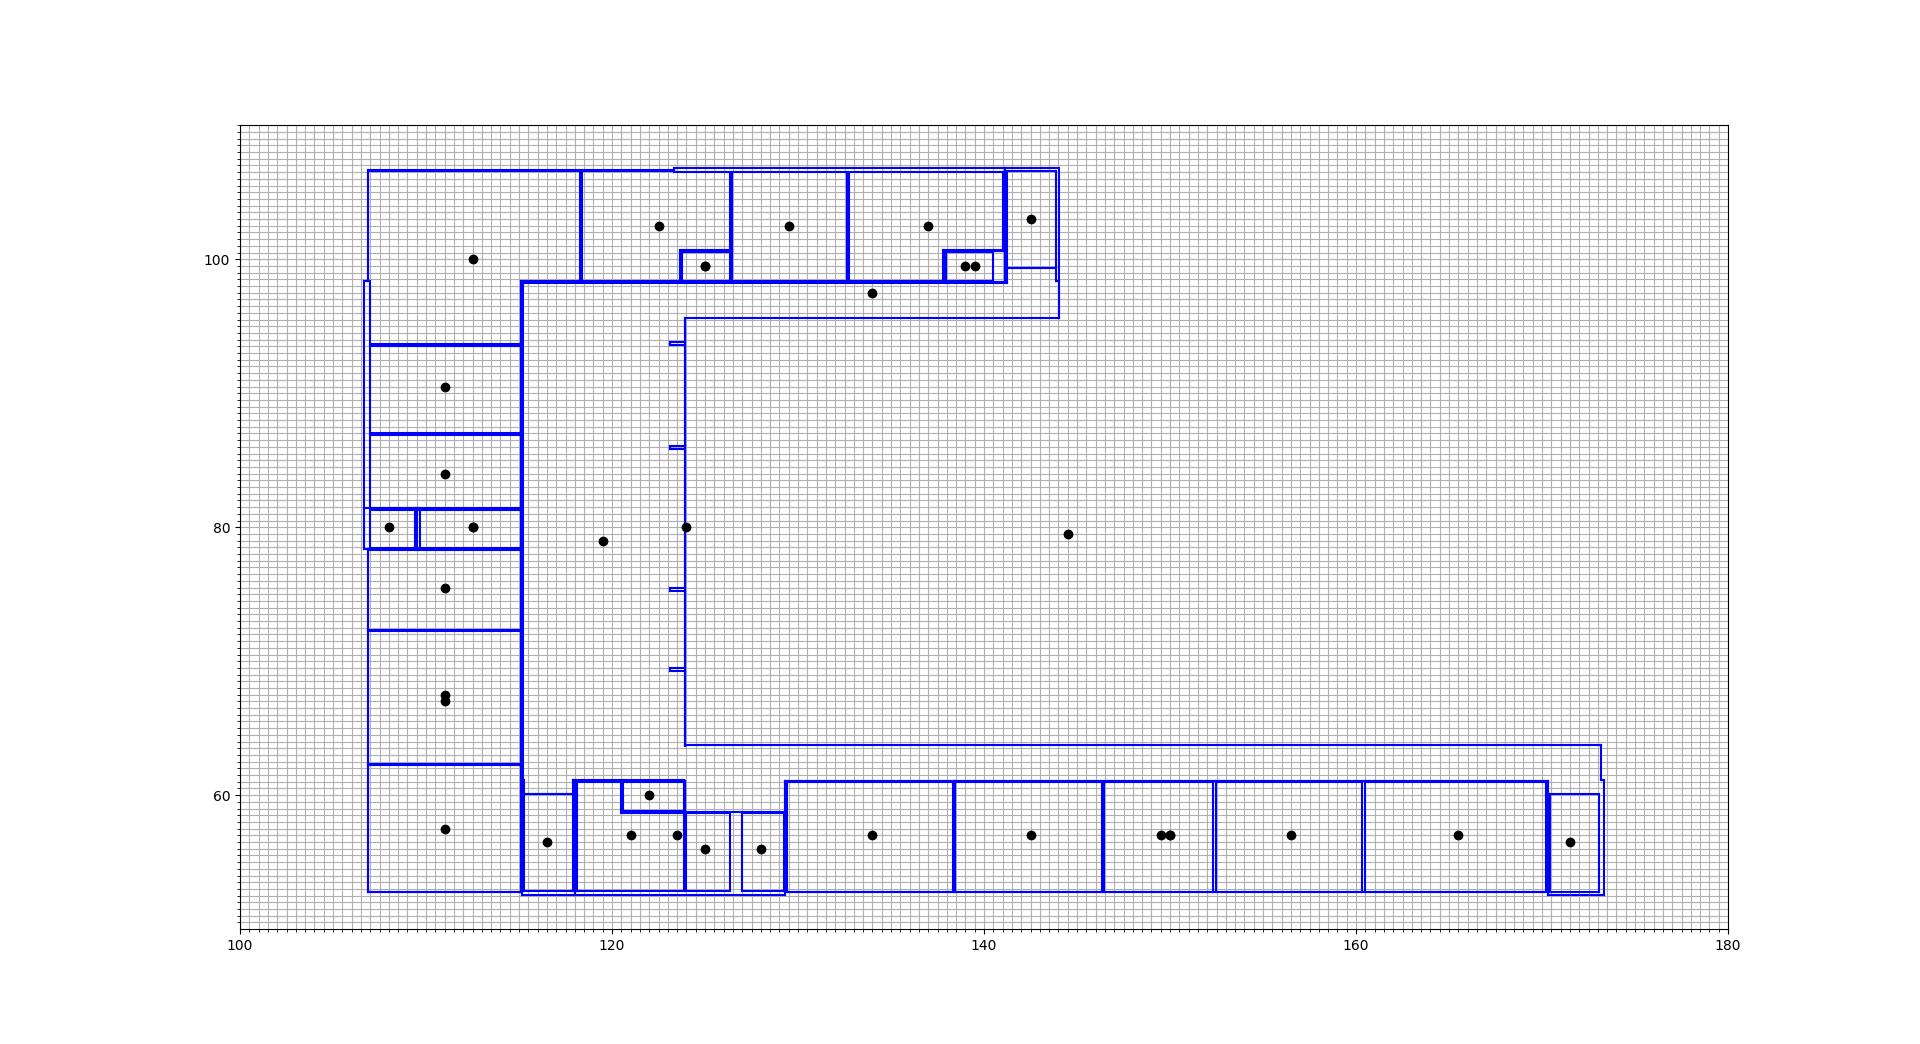
\includegraphics[width=1\textwidth]{fig/report/autogeneret_room_nodes.png}
    \label{}
    \caption[Design overview]{Example where it works somewhat well}
\end{figure}
This realisation would lead to another possible solution, namely doing convex decomposition of the rooms.


%One could achieve this by placing one room node in each room given that the rooms were convex. A convex polygon is defined by having any two nodes in the polygon being connected by a straight line without crossing the boundaries of the polygon. [show example of convex and non convex rooms] [insert reference]. The key word here is convex and for this approach to work the program would need to do a convex decomposition of all non convex rooms - which is to split a non convex polygon into convex sub polygons. Even though rooms in general are rectangle or square shaped and therefore convex, in practical applications it can be a bit complicated to do convex decomposition of non convex rooms.

%Another approach relies on the idea of generating more room nodes such that each room has multiple nodes that Spot has to visit. This would make the TSP solution slower and require Spot to walk a bit further. It would make up for it by being a much simpler method from an implementation standpoint and depending on how many nodes are being placed in each room, would still be a fairly robust solution. This was the approach that was chosen for this project. 

\subsection{Convex decomposition}
Convex decomposition of polygons is the idea of decomposing non convex rooms, to rooms that are convex. A convex polygon is a polygon where every node inside the polygon can be connect to every other node inside it with a straight line.

One solution was therefore to do convex decomposition of the rooms and place a room node at the center of each decomposed and convex room. 
The challenge with this solution was to decompose the rooms, which is the reason it in the end was not chosen as the final solution. The data did not allow for easy decomposition of the rooms, since the data is not very clean in the sense that there were a lot of lines and other things that made this approach difficult, see more in section [Data to work with].

The idea of placing optimal nodes were also an assumption that would have to be questioned and looked at from a different angle. Perhaps the best way to go about the problem would be to place a lot of room nodes and have a high probability that all corners and areas of the room would be covered. This was implemented using the K-means algorithm. 
Placing more nodes than optimal would make the TSP solution slower and require Spot to walk a bit further. It would make up for it by being a much simpler method from an implementation standpoint and depending on how many nodes are being placed in each room, would still be a fairly robust solution. This was the approach that was chosen for this project. 
%With this idea in mind the solution of doing clustering of the room nodes were chosen, more specifically the K-means algorithm.

%\subsection{K-means}
%The K-means algorithm was used to generate the room nodes.
%\begin{itemize}
%    \item Write that you are not finding the analytically best way to generate room nodes, but a discussion of this will be given in the discussion section.
%    \item The reason we need room nodes is not because we want the robot to take pictures at that spot but it is more that we want to make sure the robot visits certain areas or rooms. 
%\end{itemize}

As stated before, generating a complete room graph was needed to solve the TSP approximate solution therefore some kind of shortest path algorithm would have to be used to find the shortest distance between each of the room nodes. This shortest distance would be the weight of the edge between the nodes. There exist different shortest path algorithm but the go to standard is the A star algorithm since it is optimal and faster than many of the alternatives and it works well with grid based graph systems.

For one reason or another all the room nodes may not be connected to each other this would be due to some error with the data. Therefore before finding the shortest distance the program checks if there are room nodes that are not connected to the rest of the room nodes. If one or more of the room nodes are not connected to the rest of the room nodes these are removed.

With a complete room graph ready the program can now find the approximate TSP solution.

\begin{figure}[H]
    \centering
    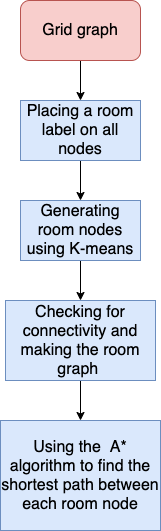
\includegraphics[width=0.3\textwidth]{fig/report/making_room_graph.png}
    \label{}
    \caption[Design overview]{}
\end{figure}



\section{TSP}
\begin{figure}[H]
    \centering
    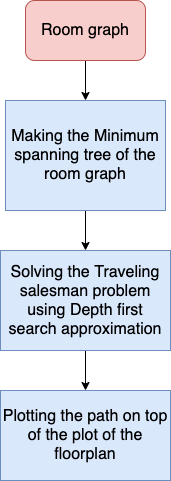
\includegraphics[width=0.3\textwidth]{fig/report/tsp_solution (1).png}
    \label{}
    \caption[Design overview]{}
\end{figure}
In this section the traveling salesman problem should be solved for the room graph. As mentioned earlier in the report an analytical solution is not needed in this case, and an approximate solution is sufficient for the purposes of this project. 
%There exist other algorithms but this one seemed to work fine.

Different approximate solution algorithms exist for TSP. A few parameters play a role when choosing which algorithm to go with. One parameter is how is the time performance, meaning how long will it take the program to run this algorithm. Another is how close to the optimal path will the solution be. The third thing to consider is how easy is the algorithm to implement given the frameworks and tools available to us.
Neither time nor performance are important factors in this program. Instead of spending a lot of time in analysis of the different algorithms and their theoretical constraints and performances the algorithm chosen in the end was chosen with ease of implementation in mind. %The 2-opt algorithm was chosen.
\begin{itemize}
    \item There are a lot of different approaches ant colony, nearest neighbour, christofides, 2-opt algorithm and others. The one went with was the 2-opt. Important that they run in polynomial time. The 2 opt is at most twice the optimal length while christofides is 1.5 optimal length, the 2 opt has shown to be around 5 \% better. Both could have been chosen, in this case I chose the 2-opt algorithm
\end{itemize}


The approximate solution used in this project is the 2-opt algorithm. 
A prerequisite of this algorithm is to have a graph that is complete, which was made sure of in the previous section.

As can be seen in \ref{TSP} the first step of the 2-opt algorithm is to make a minimum spanning tree of the graph. This is done using the Networkx library. 
The next step is to do a Depth first search traversal of the tree, again this is performed with the Networkx library. 
The final step of the 2-opt algorithm is to remove double vertices and connect the node to the next node in the tree. This is a bit more complex of a task, and the implementation of this is described in the implementation section \ref{2opt}

When the approximate solution for the room graph is found the path is transformed to the grid graph. The path information comes from doing the A star algorithm. The A star also includes the specific grid nodes traversed when finding the shortest distance from one room node to another room node. Therefore when finding the route between the room nodes this can be translated back to the grid graph. [Include figure that shows this]. This solution is then plotted on top of the plot of the floor plan, showing the final route.


\begin{itemize}
    \item how this problem is a bit different than the traditional tsp
\end{itemize}


\newpage
%\chapter{Methods}
%

\subsection{Spatial data structure framework}
As already explained the spatial data structure is a useful tool to store spatial elements in a data structure. In this program the following elements are stored in a spatial data structure:
\begin{itemize}
    \item The rooms
    \item The walls
    \item The nodes
\end{itemize}
The spatial data structure for the rooms will allow the program to access quickly which rooms each node belongs to, the usefulness of which will be discussed further here \ref{room_labels}.
The structure for the walls is used to create a buffer zone between the walls and the rest of the building. It will be used to investigate which nodes in the grid graph will have to be removed due to being too close to a wall.
Out of the three arguably the least necessary data structure is the one made for the nodes. This is used to such that the doors are connected to the closest node inside the same room as itself. 

The reason these spatial data structure are suitable to use in this project is because they allow for faster nearest neighbour search. For each of the examples explained above the use of these datastructures has made accessing the nearest room,wall or node faster and therefore the overall program faster.
Using this datastructure in this project is therefore not strictly necessary since an alternative solution that could be used is to iterate through every room,wall and node to find the nearest object. The datastructure is therefore not strictly necessary but highly advantagous to the alternative brute force solution. From a more intuitive perspective the idea of using spatial datastructures to solve a spatial problem also makes sense.  
%Since this project works on solving a geometric problem that occurs in space it is appropriate to work with spatial datastructures. 

There exist different kinds of spatial datastructures many of them work only with point objects. Due to the fact that 2 out of 3 of the objects that we wish to store in this project are multidimensional the R-tree data structure - which work with multidimensional objects - was chosen.

% The below might be better of in an implementation section
%To make the Rtree data structure was simply a matter of either implementing my own Rtree data structure class or using an existing framework, the latter option was chosen.
The framework used to make the Rtree data structure, was the Rtree module from python \cite{rtree_module}. Visit this documentation for more information on how this module works.

Although the Rtree module is designed to store multidimensional objects like rooms and wall, this data structure was also chosen to store the node objects which are not multidimensional.
This might not be the optimal way to store point objects but to simplify the program and minimize the number of different frameworks used in the program the Rtree was also chosen for this datatype. Using another spatial data structure for the point objects is a very reasonable alternative.



\subsection{Room labels}\label{room_labels}
In order to generate the room nodes of the room graph it is necessary to first label each grid node to the room it is inside of. 

The way it works is that we iterate through each node in the grid. We then find the nearest rooms to the grid using the R-tree generated for the rooms. Sometimes due to the way the data is formatted a node can be inside multiple rooms at the same time. Therefore the program finds the area of the rooms and sort them such that the node is tested to be within the smallest room first. This is because the rooms are sometimes inside each other.
When checking if the node is inside the room the ray casting algorithm is used together with line intersection. In theory it should be enough to check one direction to decide whether the node is within the room or not. This is not the case here however, mainly due to the fact that other elements are included in the floor plan. One example are pillars that can be present in the floor plan and could therefore interfere with the line intersection. 
Therefore 4 directions are checked and a majority voting system is used to decide whether the node is inside or outside the room.
If a node is not inside any rooms it is removed from the graph since this means that it is outside the building and therefore shouldn't be a part of the path under any circumstances.

\begin{itemize}
    \item Talk about why it is important and needed
    \item How to make sure that the path doesn't go outside the building
    \item Write about the special case where you wouldn't be able to remove outside nodes if there is a yard inside the building
\end{itemize}


\subsection{Node placement}
Looking at the objective \ref{Objective} it is seen that the next step is to generate the room graph. 
Different options existed for generating the room nodes that made up the room graph. One option and the option that was used in the end was to use a clustering algorithm to generate the nodes. Specifically the K-means algorithm.
This was with the idea that finding an analytically optimal position for the room nodes would be cumbersome task compared to finding an approximate solution. Another way was to use convex decomposition. Autogenerate nodes.

\begin{itemize}
    \item the reason we need room nodes is not because we want the robot to take pictures at that spot but it is more that we want to make sure the robot visits certain areas or rooms. 
    \item Write that when using the k means sometimes the centroids fall out of the room, in that case we just choose a random centroid in the room.
    \item Write about different ways to place the room nodes, like taking the center point of the room, and why that is not always a good idea. Convex decomposition.
\end{itemize}








\begin{comment}
\subsection{Minimum spanning tree}
This is a one line code that makes a minimum spanning tree given a network. This comes from the networkx framework. 
The minimum spanning tree is needed to do the approximate solution of the tsp problem.

\subsection{Solve TSP problem for subgraph using DFS traversal}
This is again a one line of code, where a depth first search traversal is performed on the minimum spanning tree of the rooms. 

The next step to finalize the tsp solution is to remove double vertices occuring when doing the depth first seach algorithm on the minimum spanning tree.



The dfs list consists of node pairs with a 'from' node and a 'to' node.
e.g
(1,2), (2,3), (3,4) etc.
We can have that the 'from' node of the current node pair is not the 'to' node of the previous node pair. 
e.g
(1,2), (1,3)
When this happens we want to make i a shortcut such that it goes directly from 2 to 3 without going back to one.


We do this by having a for loop that runs through all node pairs in the list of the depth first search edges. 
If the 'to' node in the previous node pair
is not the same as the from node in the next node pair then the new 'from' node should be the previous 'to' node and the new 'to' node
should be the current 'to' node.
For example if we have (1,2), (1,3) then because we go back to 1 we change it to (1,2), (2,3).


\begin{itemize}
    \item Making a weighted graph of all the nodes, where the weights are the Euclidean distance between each node. Write that it is a undirected graph.
    \item A section on the line intersection algorithm used for connecting the points
    \item Using dijkstra's/A* to make a complete subgraph of all the relevant nodes, and how this problem is a bit different than the traditional tsp.
    \item Removing double vertices to do the DFS traversal algorithm
    \item Plotting the final solution
    \item Checking for connectivity between the room nodes
    \item Write about the different ways you wanted to plot the path. Not just Distance field but the alternatives. Corner approach. Various sized of grid, like in the video game video.
\end{itemize}

\subsection{Line intersection}
When determining whether to points on a map are traversable some sort of line intersection algorithm is used. Without using
line intersection the program wouldn't be able to detect whether there are walls between two points, and it would therefore always
choose the shortest distance between two points to be a straight line, regardless if it passes through walls or not. 
(insert reference https://bryceboe.com/2006/10/23/line-segment-intersection-algorithm/)
The algorithm chosen in this case works by checking first if three points are counterclockwise of each other.
\end{comment}


%\newpage
\chapter{Implementation}
\section{Software to use}
\begin{itemize}
    \item Ros, unity and python.
\end{itemize}

\section{The specific data format / The data given}
As written in \ref{dataset} the data is of the IFC format. Actually the data is generated by Dalux from the IFC format. Dalux takes the IFC data of a building and passes it through their parser that generates 5 xml files: rooms.xml, floorplaninfo.xml, levels.xml, structure.xml and properties.xml and generate one .txt file named: output.txt. Therefore this project does not actually work with any IFC file.
The rooms.xml file has information about the rooms in the floor plan. Basically the floor plan is generated as a collection of rooms. The coordinates of the rooms are triangles spanning the room. Each room has associated with it its minimum elevation level and its maximum elevation level which represent the height of the floor and the height of the ceiling of the room. These elevation levels are the ones used to choose which rooms to include in the floorplan.

The floorplaninfo.xml file has information about the doors of the rooms. For each door the file has information about its origin point i.e the coordinate placement of the door. Furthermore it has information about the height of the door. It also has information about the direction that the door is facing, given as a unit vector.

In the output.txt file information about the translation is given. In some buildings this is needed to translate the door coordinates so that they align with the floorplan. [insert picture of them not aligning]

The rest of the files are not used in this project since they consist mostly of semantic information of the building.

In normal circumstances an IFC loader could be used to load IFC files. Since in this case the files are not IFC files but are Dalux' own data format derived from IFC files, a separate loader had to be constructed. 




\subsection{Loading the data}
The overall program consists of 3 scripts: read\_write.py, coordinate\_processing.py and plotting\_data.py.
The script read\_write.py is used to load the data. It takes the floor plan data as input and uses the xml.etree.ElementTree module to append the coordinates of each room to a list and the coordinates of the doors to another list. Both lists are parsed to a csv file.

%\subsection{Preprocessing of the data set}
Before working with the data set some preprocessing had to be done. This included splitting the array values in appropriate ways and gathering them in sets of three such as to align with the triangles they would form. The coordinate\_processing.py module was made to handle this.


\section{Plotting floor plan}
It is always a good idea to get an overview of the data used in a project. This is especially the case in this project since the data in this case is a visual representation of something physical - a floor plan of a building. It therefore made sense to find a good way to transform the data from its original form to a plot that visualises how the floor plan looks. This will be useful throughout the project because it will act as a clear visual indicator of potential errors occurring in the program; we will quickly see if a path goes through a wall or if door nodes are not placed where they should be placed. This would not be the case if we omitted to plot the floor plan and only plotted the graph and the route.
\\\\
A random floor is chosen among the different floors of the building. This is done by checking the MinimumElevation value given in the rooms.xml file. For each room if it has a specific minimum elevation value the program keeps the room. 
%\subsection{Plotting the doors}
\\\\
When plotting the doors a challenge occurred, which was that a transformation had to be performed on the doors before they were aligned with the rest of the floor plan. This would only sometimes be the case. The information about the translation could be found in the output.txt file.
\\\\
For the doors a csv file is constructed which consists of the coordinate of each door and the direction it is facing. The last line of the csv file includes the coordinate translation.
\\\\
For each door point a complementary door point will be added. This complementary door point will be  added on the other side of the wall that the original door point is facing, using the direction information of the doors. This makes it possible to go through walls when solving for the path, since complementary doors always will be connected.
\\\\
The correct doors are chosen for the right floor plan using the height information related to the doors. These do not always match in scale and a translation will on some buildings have to be performed. The program checks if this is needed.

\begin{itemize}
    \item Talk about difference between using minimum elevation or clippingHeight.
\end{itemize}


\subsection{Removing redundant lines}
The triangle structure of the data set forms a mesh that spans the entire floor plan. If just plotted as is this does not do a great job of visualising the floor plan in an appropriate way, since a lot of unwanted lines will be there. [insert figure of the floor plan with triangles]. Some processing has to be done to remove these unwanted lines and make the rooms in the floor plan distinguishable from each other. The idea of how to go about this problem came from \cite{wayfinding} where they also met the same challenge. The intuition behind their idea was that the lines to be removed are part of more than one triangle, if e.g two triangles are used to span a room the line that should be removed is the one shared by both triangles. In order for this to work each line had to be hashed. There are some slight modifications to the way hashing is performed in this project compared to their project. In this project each line is hashed, where they hash each point in their project.

[insert flowchart of the process of hashing, and also a sketch describing it]

\begin{itemize}
    \item Explain that we wish to remove lines of the shared triangle. Insert a sketch that explains what we want to do.
\end{itemize}

%For each triangle the program hash all lines in that triangle in a dictionary in both direction. This means that we hash 6 lines per triangle. The reason for this is that a triangle might have the same line as another triangle but in reverse order. These two lines should be seen as the same. Therefore we have to hash both directions of each line in every triangle.

%For example say we have a line in one triangle (x1,y1) - (x2,y2). What might be the case is that another other triangle might have the same lines as the first triangle but as (x2,y2) - (x1,y1). Therefore the program hashes the line (x2,y2)-(x1,y1) as well. Just like the other triangle both directions will be hashed meaning (x1,y1)-(x2,y2). The way hashing works is that two identical values will give the same hash key. In this example we now have two values for two different hash keys, since the same line is occuring twice in two different hashes.

%Now each dictionary element that has more than one value is removed. Therefore both of the hashes will be removed and we have made sure that the line is correctly removed.
%The way we hash also has the consequence of having each line existing twice in the dictionary. Therefore one of the directions of each line is removed. This makes the dictionary half as long and makes it more efficient for use later if need be.

%%The idea here is to make a dictionary where each line a set of two point coordinates is given a key and the same lines will have the same key. For example the point set of The way to make sure that the same lines will get the same key is by using hashing. Then all keys with more than one value (line) will be removed. The idea of using hashing to remove redundant lines was taken from this project (insert project reference).

\section{Spatial data structure framework}
As already explained the spatial data structure is a useful tool to store spatial elements in a data structure. In this program the following elements are stored in a spatial data structure:
\begin{itemize}
    \item The rooms
    \item The walls
    \item The nodes
\end{itemize}
The spatial data structure for the rooms will allow the program to access quickly which rooms each node belongs to, the usefulness of which will be discussed further here \ref{room_labels}.
The structure for the walls is used to create a buffer zone between the walls and the rest of the building. It will be used to investigate which nodes in the grid graph will have to be removed due to being too close to a wall.
The least necessary out of the three data structures is arguably the one made for the nodes. This is used to such that the doors are connected to the closest node inside the same room as itself. 

The reason these spatial data structure are suitable to use in this project is because they allow for faster nearest neighbour search. For each of the examples explained above the use of these datastructures has made accessing the nearest room, wall or node faster and therefore the overall program faster.
An alternative brute force solution that could be used is to iterate through every room, wall and node to find the nearest object. The datastructure is therefore not strictly necessary but highly advantageous to the alternative brute force solution. 
%From a more intuitive perspective the idea of using spatial datastructures to solve a spatial problem also makes sense.  
%Since this project works on solving a geometric problem that occurs in space it is appropriate to work with spatial datastructures. 

There exist different kinds of spatial datastructures though many of them work only with point objects. Due to the fact that 2 out of 3 of the objects that the program wish to store are multidimensional, the R-tree data structure - which work with multidimensional objects - was chosen.

% The below might be better of in an implementation section
%To make the Rtree data structure was simply a matter of either implementing my own Rtree data structure class or using an existing framework, the latter option was chosen.

The framework used to make the Rtree data structure, was the Rtree module from python \cite{rtree_module}. 
%Visit this documentation for more information on how this module works.

Although the Rtree module is designed to store multidimensional objects like rooms and wall, this data structure was also chosen to store the node objects which are not multidimensional.
This might not be the optimal way to store point objects but to simplify the program and minimize the number of different frameworks used in the program the Rtree was also chosen for this datatype. Using another spatial data structure for the point objects is a very reasonable alternative.


\section{Sampling the graph}
%Making a graph to represent the path and the places that Spot should visit was from the start the very straightforward way to go about the problem. 
The standard framework used when working with graphs in python is the Networkx library. This was also the framework chosen in this program to work with graphs.
As explained in \ref{design} Making a grid graph was chosen to represent the building with a resolution of 0.5x0.5 for x and y direction. The reason behind this resolution was that it would allow the entirety of Spot to fit within each node of the graph. This way each node could either be deemed traversable or not traversable by Spot.

Each node created in the graph would have the following attributes associated with it: the point coordinate, the distance to the closest wall, the node type i.e is it a door node or grid node. Later when doing the room labeling, the room number would also be an attribute to the node. 
The distance to the closest wall could be found by making use of the R-tree generated for the walls. The motivation behind including this attribute was to be able to remove the nodes that were within a certain distance to the closest wall. Including the coordinate of the node was also necessary in many different sections of the program. The same with the node type labeling. Furthermore an R-tree data structure for the nodes would also be implemented while generating the grid nodes.

Since the graph would be as a grid each node would have an edge to eight other nodes in the grid. Knowing the length of the columns of the grid it was possible to connect each node to a the node diagonal, vertical and horizontal to it. 

\begin{itemize}
    \item Explain how exactly you managed to connect the nodes
\end{itemize}

When all the nodes would be generated the nodes within a certain distance of the walls would be removed along with their edges.

\subsection{The door nodes}
Originally the doors were also discretized to fit into the grid, which would move the doors to the closest grid point. This showed itself to be problematic because the doors would move to another position than they were actually placed. 
There were a few problems with this. One was that it could cause problems when Spot would want to walk through the door and the door would actually be a maximum of 25 cm away from its actual position. This was somewhat concerning but might still have been a durable solution since Spot has the ability to detect obstacles and move around them and therefore might have been able to move through the door anyway.
The bigger issue with discretizing the doors was that the doors would sometimes move just enough that they no longer were connected to the same room. Although this was a rare occurrence it could pose a big problem in the robustness of the program.

With these two things in mind it was decided to not discretize the doors, and thereby keep undiscretized doors in a discretized grid, at the cost of complicating the program a bit.

The doors would have edges to only two nodes in the graph, one would be its complementary door node and the other node would be the closest node with the same room label as the door node. 
%Which leads to the next section.

%After I remove nodes near the walls, (and before I remove door nodes that are outside the building) I check for each door whether or not it is connected to more than one other node. If it is only connected to the 1 other node it means that it is only connected to its complementary door. In this case the door should connect itself to a random node in the room. In this case the program should connect the door to the nearest node that is not crossing a wall. I need a spatial data structure for the nodes.


\section{Room labels}\label{room_labels}
In order to generate the room nodes of the room graph it is necessary to first label each grid node to the room it is inside of. [Insert flowchart that illustrates the algorithm and heuristic]

The program iterates through each node in the grid and finds the nearest rooms to that node using the R-tree generated for the rooms. Sometimes due to the way the data is formatted a node can be inside multiple rooms at the same time. Therefore the program finds the area of the rooms and sort them such that the node is tested to be within the smallest room first. This is because the rooms are sometimes inside each other.
When checking if the node is inside the room the ray casting algorithm is used together with line intersection. In theory it should be enough to check one direction to decide whether the node is within the room or not. This is not the case here however, mainly due to the fact that other elements are included in the floor plan. One example are pillars that can be present in the floor plan and could therefore interfere with the line intersection. 
Therefore 4 directions are checked and a majority voting system is used to decide whether the node is inside or outside the room.
If a node is not inside any rooms it is removed from the graph since this means that it is outside the building and therefore shouldn't be a part of the path under any circumstances.

Labeling the rooms serve a few functions. One of the places that it is used is when generating the room nodes using the K-means algorithm. Without knowing how many rooms there are or knowing which nodes belong to which rooms, we can not make sure that each room has a minimum of one room node associated with it.
One of the other functions of the room labeling is that it removes nodes that are outside the building. This is because outside nodes will not be part of any rooms, and are as a result removed. Doing this insures that Spot does not traverse outside the building. [Show example where it traverses outside the building]


There are some special cases where this algorithm will not remove outside nodes. This could for example be the case if the building consisted of a yard inside of it. [insert a sketch] Depending on how the architect labeled the rooms this could be an issue. The counter argument would then be that it might not be a problem for Spot to be walking in the yard in that case since the yard is part of the building. It might also allow for a faster traversal through the building. 

\section{Node placement}
As explained in \ref{room_graph} Different options exist for generating the room nodes that made up the room graph. One option and the option that was used in the end was to use a clustering algorithm to generate the nodes, more specifically the K-means algorithm. 
The K means algorithm was implemented and the number of centroids were chosen by a ratio of the number of nodes in the room. This way bigger rooms would have more centroids i.e. room nodes. In the case that the centroid falls outside the room a new centroid is chosen randomly from the nodes in the room. The K-means stops after five iteration, and after one iteration if there is only one room node in the room. 

%One could choose a more sophisticated convergence criteria, but this was not deemed necessary since finding the perfect spot for the centroids were not important.
\begin{itemize}
    \item Exlain other convergence criteria.
\end{itemize}
%\section{Making sure that doors are connected to nodes in room}

%\section{How to choose the correct doors and floorplan}

%\section{Choosing the floorplan}
%- rooms are in other rooms.

%\section{Bugs and challenges}
%- Make a list of all the challenges and bugs and write a section for each of them.


\subsection{Connecting the room graph}
%To make a graph placing the nodes are not the only thing needed to be done, adding the edges is also necessary. 
To solve the TSP approximate solution for this graph a prerequisite is to make the room graph complete. Therefore edges between all nodes in this graph were to be added.
However before doing this, as a robustness check the program checks if all of the room nodes are connected. This is done using the Networkx library which has a function that can check how many nodes need to be removed before there is no longer connection between two nodes, if this number is zero it means that the two nodes are not connected. The room nodes that are not connected to the rest of the graph are removed.
After making sure that the nodes are indeed connected it is time to create edges between the nodes. The weight of the edges were found by finding the shortest path between each of the nodes. This was found using the A star algorithm. 

%\begin{itemize}
%    \item Are there different ways to do this?
%\end{itemize}

\section{Tsp solution}

\begin{itemize}
    \item How was this exactly implemented
\end{itemize}




\section{What the data lacks}
A big challenge to the program occurred when there were walls in the floor plan that seemed misplaced. Investigating the 3D model of the building it seemed that these walls were not supposed to be there. The distinction between what is illustrated in the 3D model and what is shown when the program plots is caused due to the fact that not all information from the BIM model is parsed to the six files generated by Dalux. 

There is no information in the data that indicates which lines represent walls and which lines do not represent walls. As a general case every line on the floor plan represent walls but this is not always the case. It depends on how the architect decided to design the building. Take for example the following building [insert figure], here these rooms are in reality one big open space, but the designer deemed it useful to separate this open space into three rooms and therefore there are lines separating the rooms. 

The issue as can be seen in the figure below [insert figure] is that since these lines will not have doors connected with it they will result in blocking of the path. Spot might therefore not be able to traverse to all the rooms in the floor plan.

A big portion of energy was used to reconcile this distinction between what is plotted and what is actually the case and find ways to tackle this issue. Since there is no information given in the files about which lines represent walls, a heuristic had to be found solve the issue.



\subsection{One wall algorithm, walls that are not supposed to be there}
From investigating the difference between the lines that were supposed to represent walls and the lines that were not supposed to represent walls a realisation came. It seemed that the walls separating the rooms often consisted of two parallel lines with a small separation between the lines. This seemed to indicate the thickness of the wall. The reason for these double lines comes from the fact that when the rooms are generated they do not share lines. On the other hand it seemed that when there was not supposed to be this line separation the two rooms shared the same wall. Another way to view this was that the line represented a wall with thickness 0.

With that in mind a heuristic was implemented that would check all rooms if lines were overlapping or shared. 
This was done by comparing line for line in two for loops. 
There are two scenarios where the wall can be removed. 
The first scenario is if the two line segments are identical.
The second scenario is if the line segments are overlapping i.e. one line segment is a part of another line segment.
[insert figure of different scenarios]

This is done by checking the slopes of the points making up the line segments, if the slope of all the points of the two line segments are the same it means that they are co-linear. This does not necessary mean that they are overlapping. To figure this out a projection on the x axis is performed. In the special case of vertical lines a projection on the y-axis is performed. If  one of the points of one line segment is overlapping with the other line segment this means that the line segments overlap [insert figure]. 
Before removing the line segment we check if there are doors within a certain distance of the wall. This is because we do not want to remove lines that have doors connected to it since this means that the line is actually a wall or that the doors are supposed to be used to traverse the line.

The results of using this heuristic were not perfect as can be seen from the results section \ref{results}, they were however an improvement to not using it.


%In this project a loader was made to load the data and plot it. It is worth saying that there are alternative pre-made loaders to do this. For example [IFC open shell loader, insert reference]. I chose to make my own loader because at the time it seemed like the straight forward thing to do. I was assured that the data was made in a certain way by Dalux, and since the data was given in a specific format and consisted of a small part of what a true IFC file consists of I decided to make my own loader. If the user wants to use this program for general IFC files it is simply a matter of using a already existing IFC loader, like the one mentioned earlier.
\newpage
\chapter{Results}

\begin{itemize}
    \item Write the results for the RAC building.
    \item Find a system to judge it on.
    \item Mention whether there is or is no ground truth
    \item Manuel planning of route
    \item the results are run on the same script with no of the script between each building. THe only thing changed is the name of the building used.
\end{itemize}
\begin{comment}

\begin{figure}[H]
    \centering
    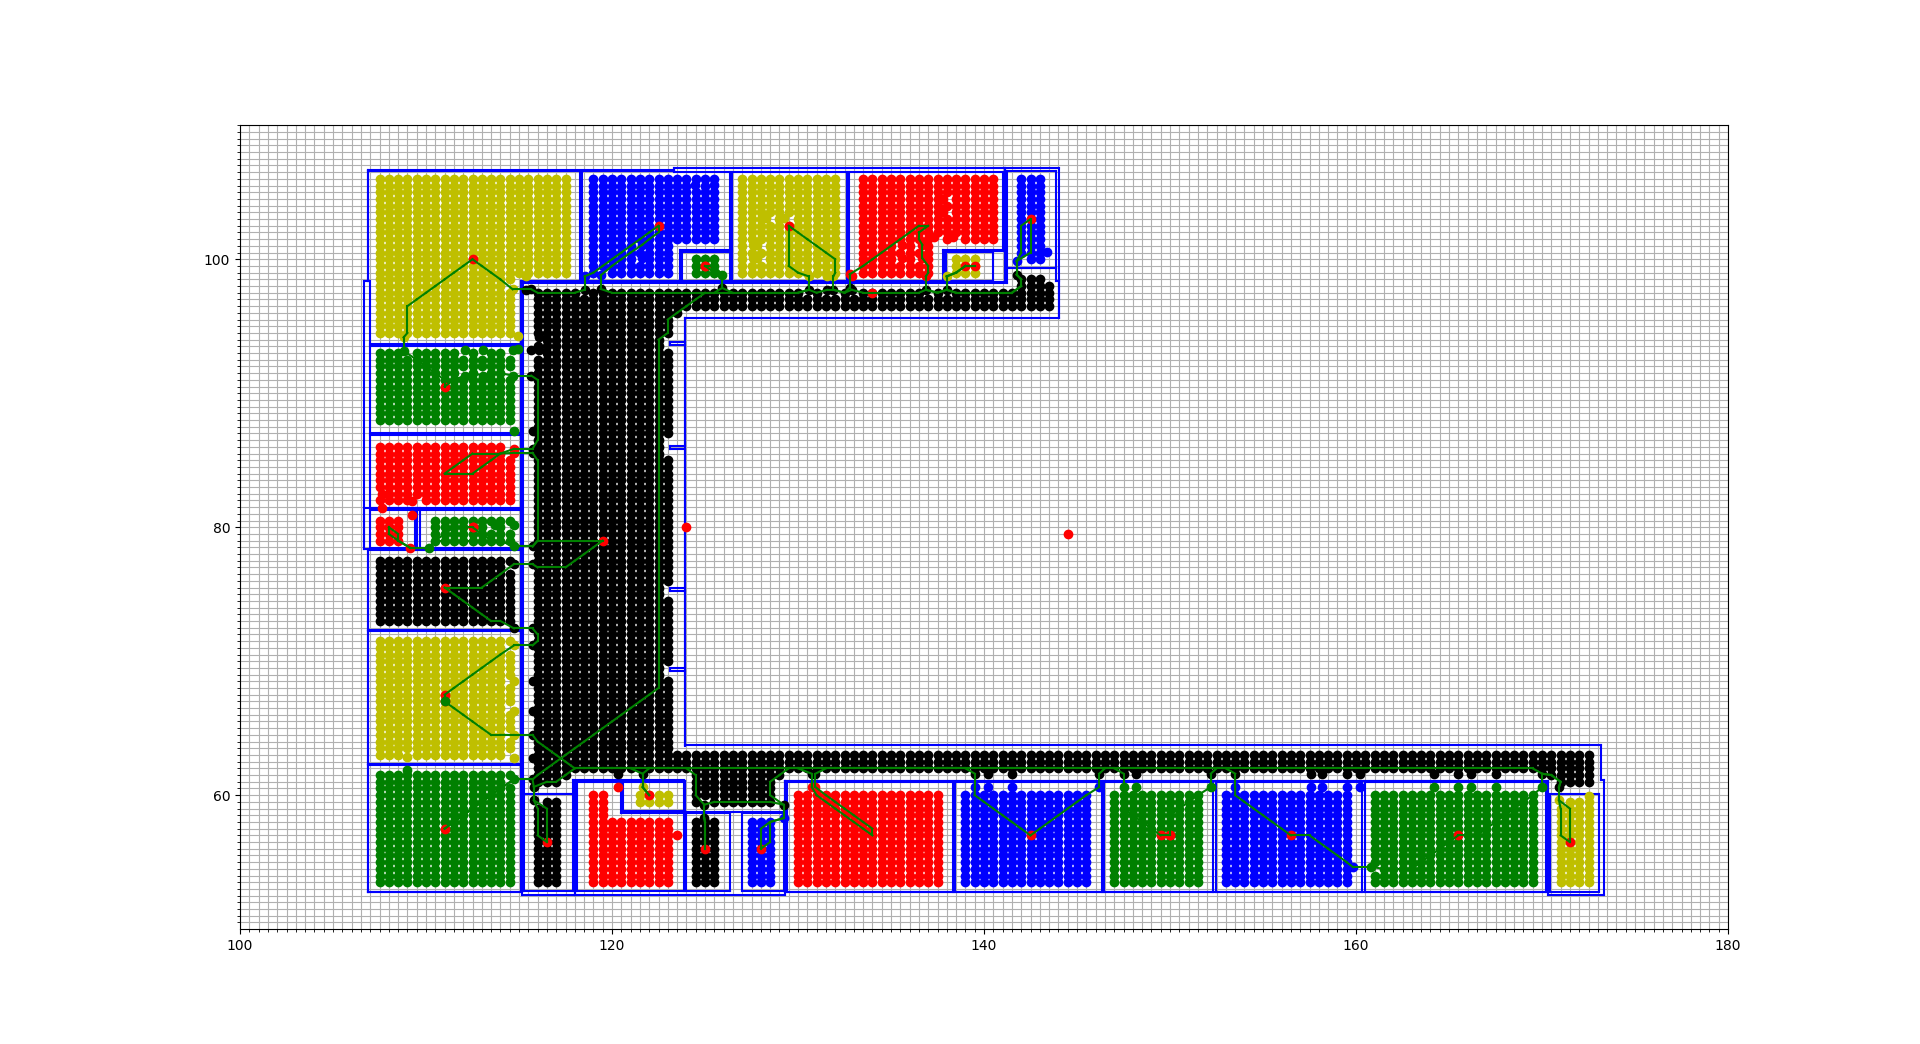
\includegraphics[width=1\textwidth]{fig/rum_labels.png}
    \label{}
    \caption[Design overview]{Rum knudepunkter}
\end{figure}


\begin{figure}[H]
    \centering
    \includegraphics[width=1\textwidth]{fig/hele_første_floorplan.png}
    \label{Rum knudepu}
    \caption[Design overview]{}
\end{figure}
\end{comment}


\section{RAC}
Comparing how the doors are plotted.
\begin{figure}[H]
    \centering
    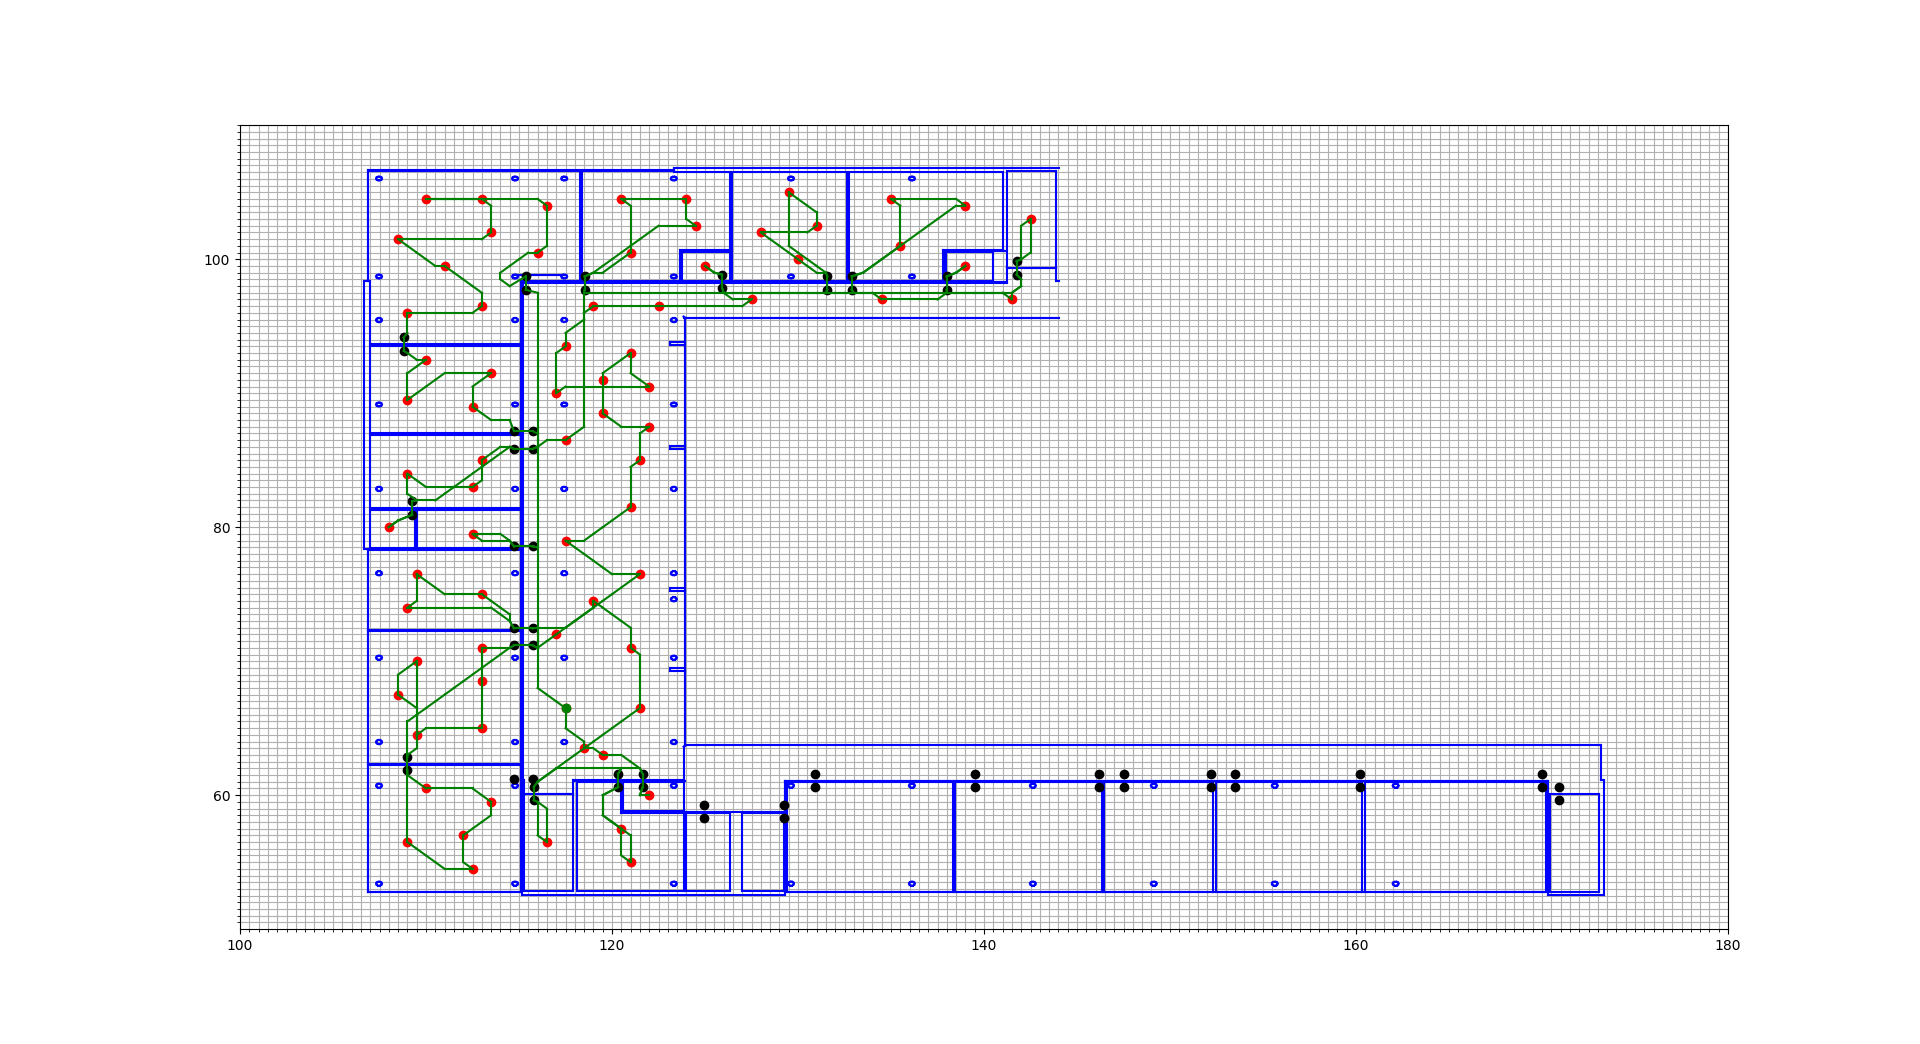
\includegraphics[width=1\textwidth]{fig/Resultater/Rac/-2.154_min_height_radius0.01.png}
    \label{Rum knudepu}
    \caption[Design overview]{}
\end{figure}


\begin{figure}[H]
    \centering
    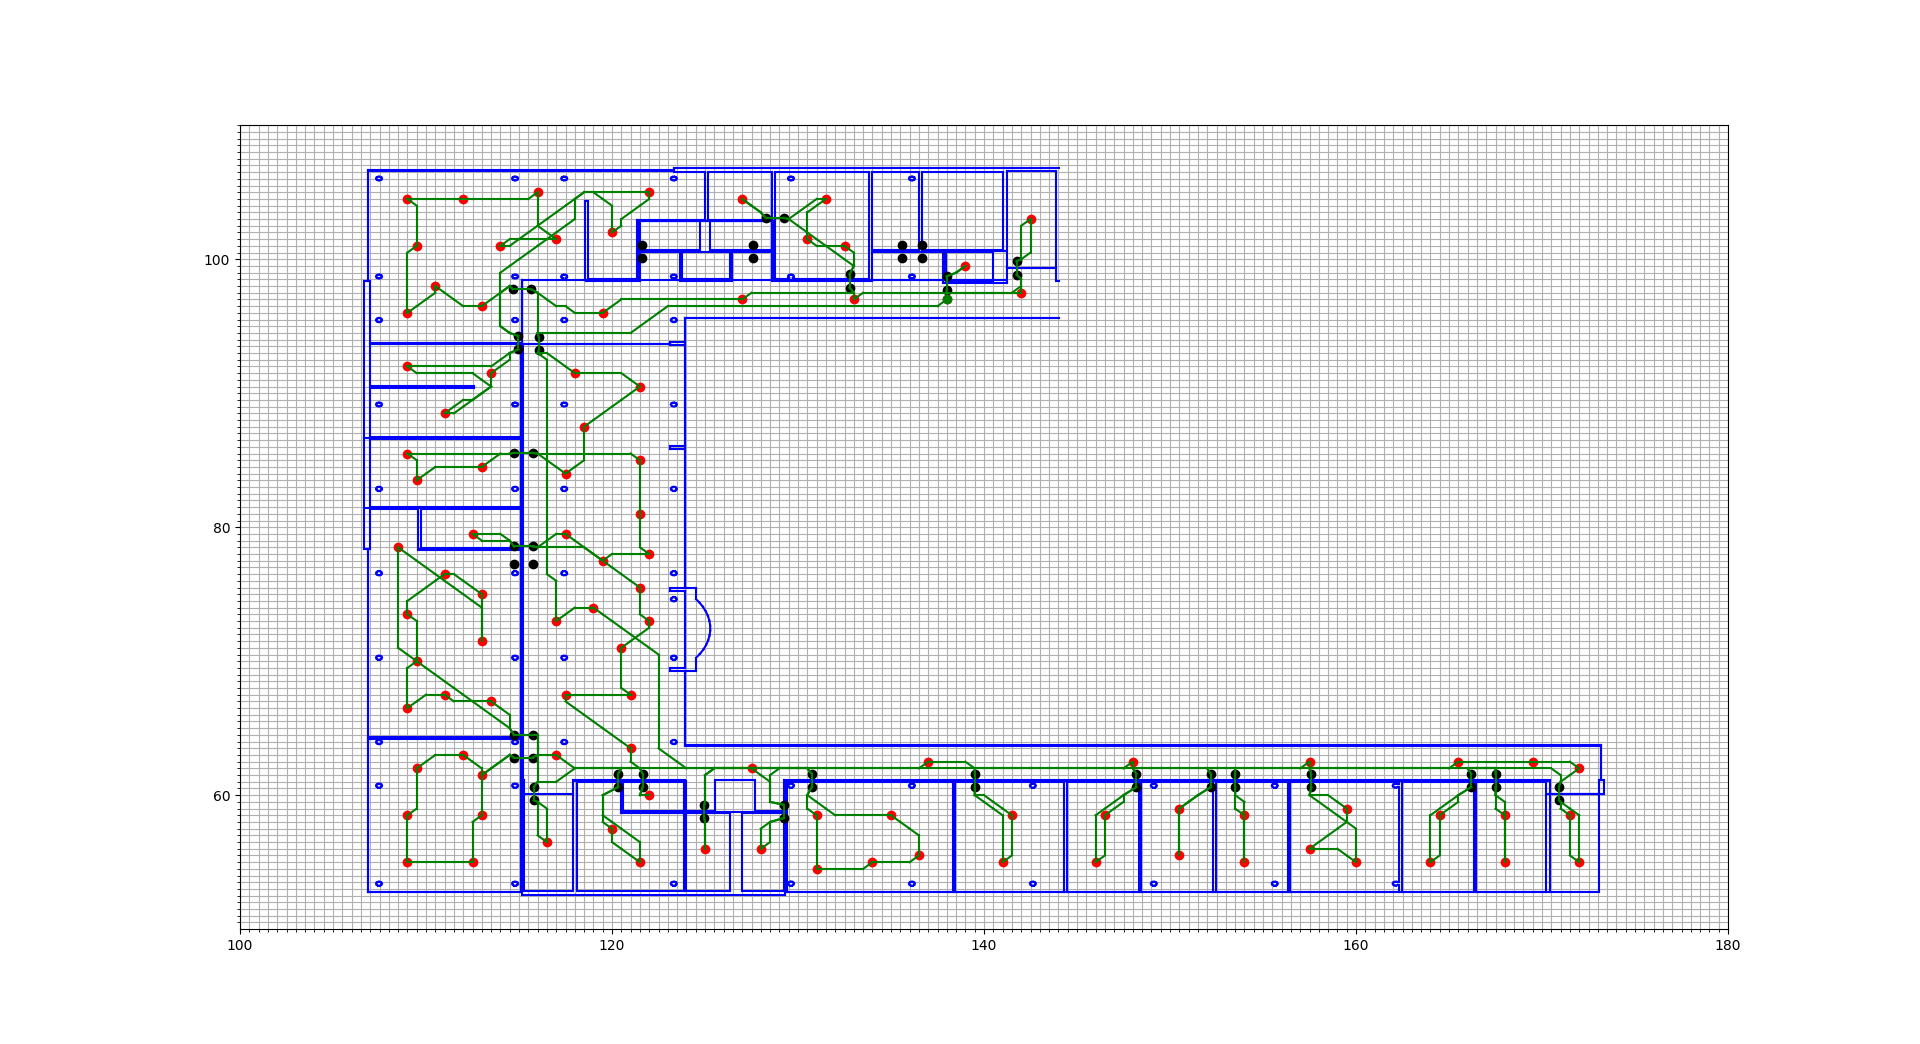
\includegraphics[width=1\textwidth]{fig/Resultater/Rac/-5.95_min_height_radius0.01.png}
    \label{Rum knudepu}
    \caption[Design overview]{}
\end{figure}


\begin{figure}[H]
    \centering
    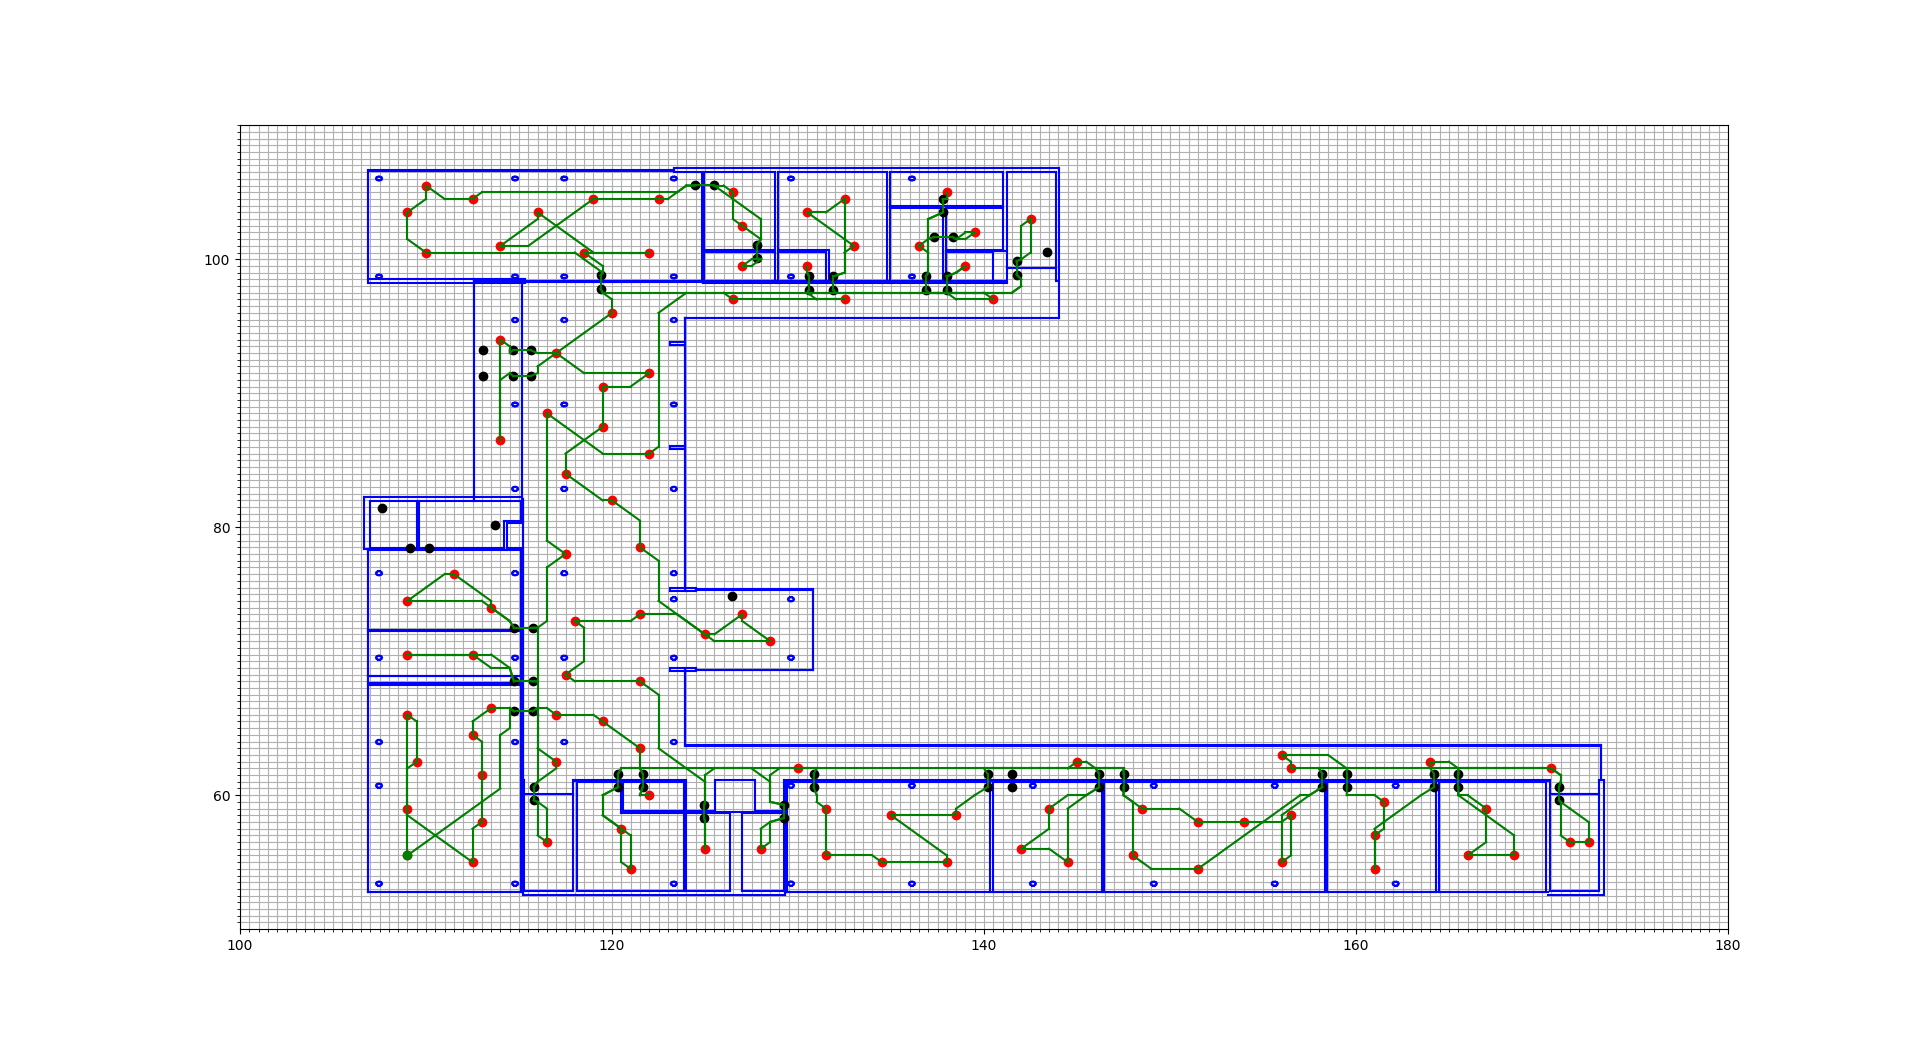
\includegraphics[width=1\textwidth]{fig/Resultater/Rac/-9.7_min_height_radius0.01.png}
    \label{Rum knudepu}
    \caption[Design overview]{}
\end{figure}


\section{Building 127}
- Checking 3 radius of different number of doors included.
How will the plotting work.
\begin{figure}[H]
    \centering
    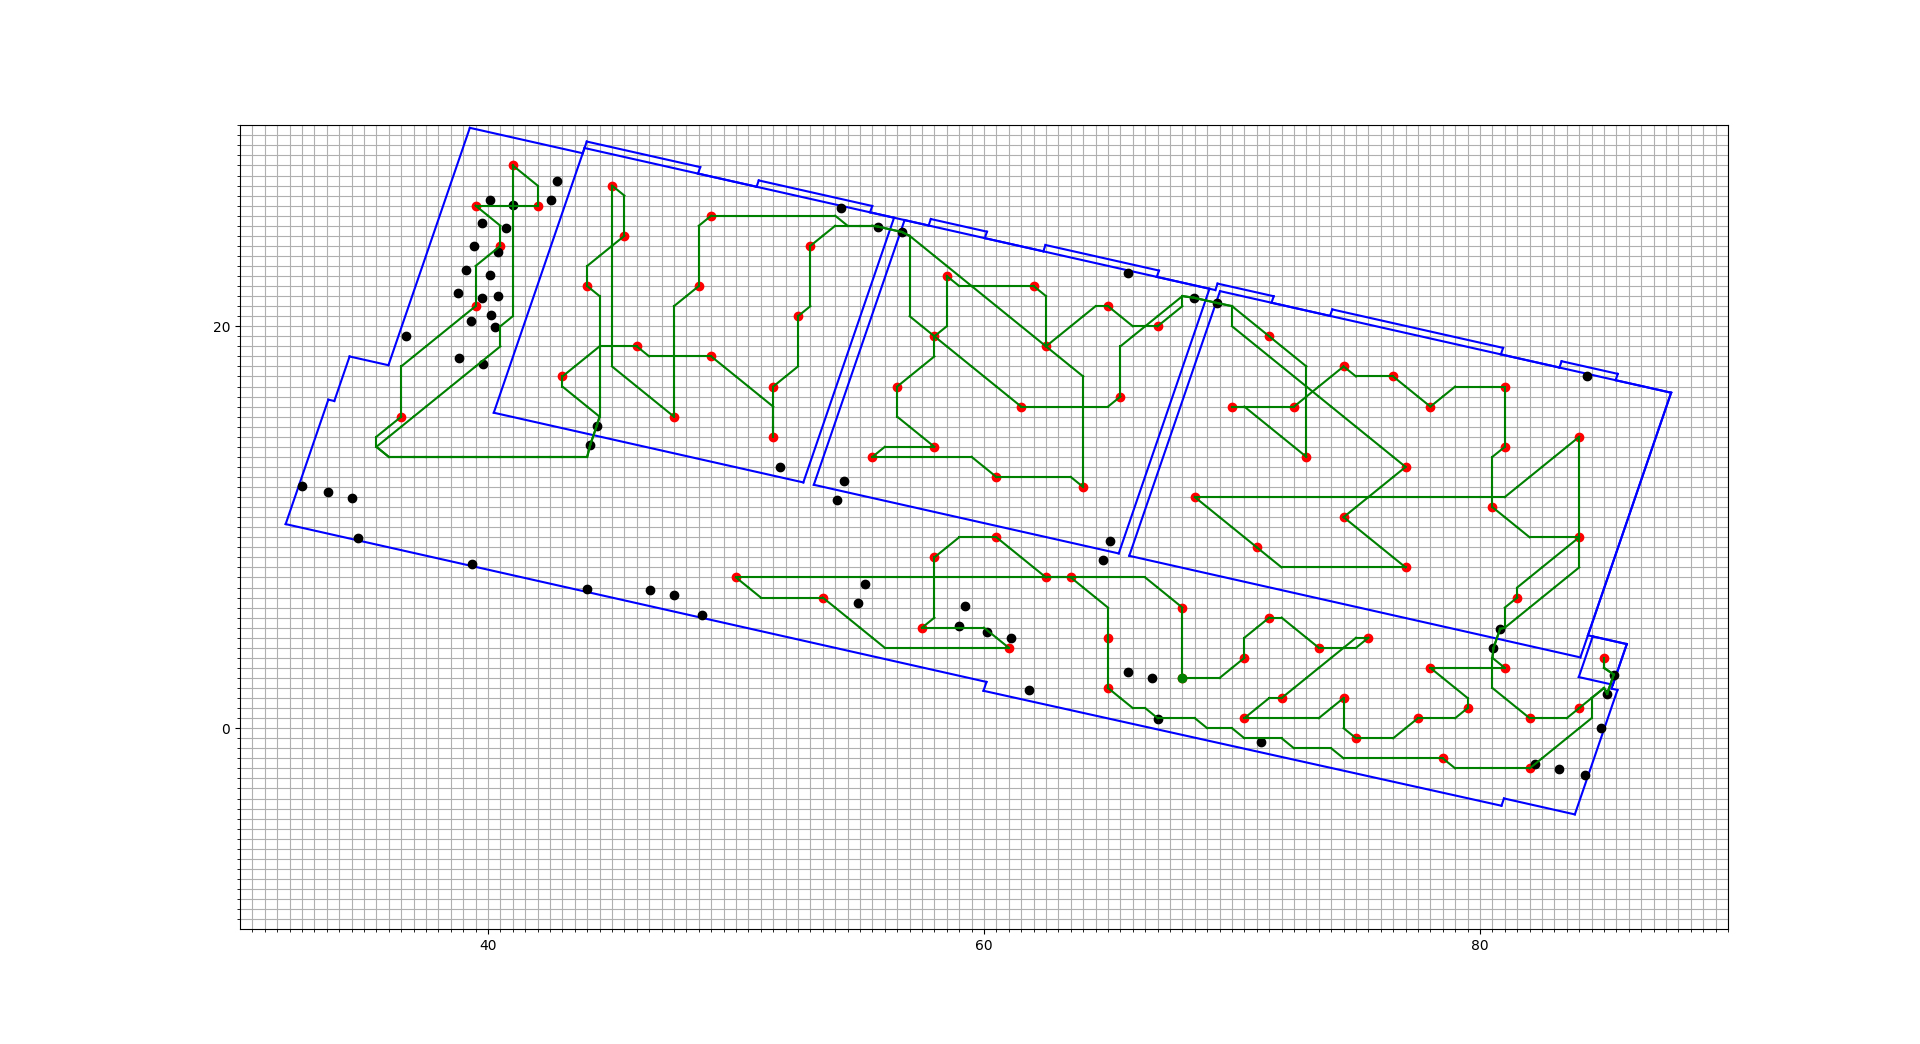
\includegraphics[width=1\textwidth]{fig/Resultater/127/0.31_min_height.png}
    \label{Rum knudepu}
    \caption[Design overview]{}
\end{figure}

\begin{figure}[H]
    \centering
    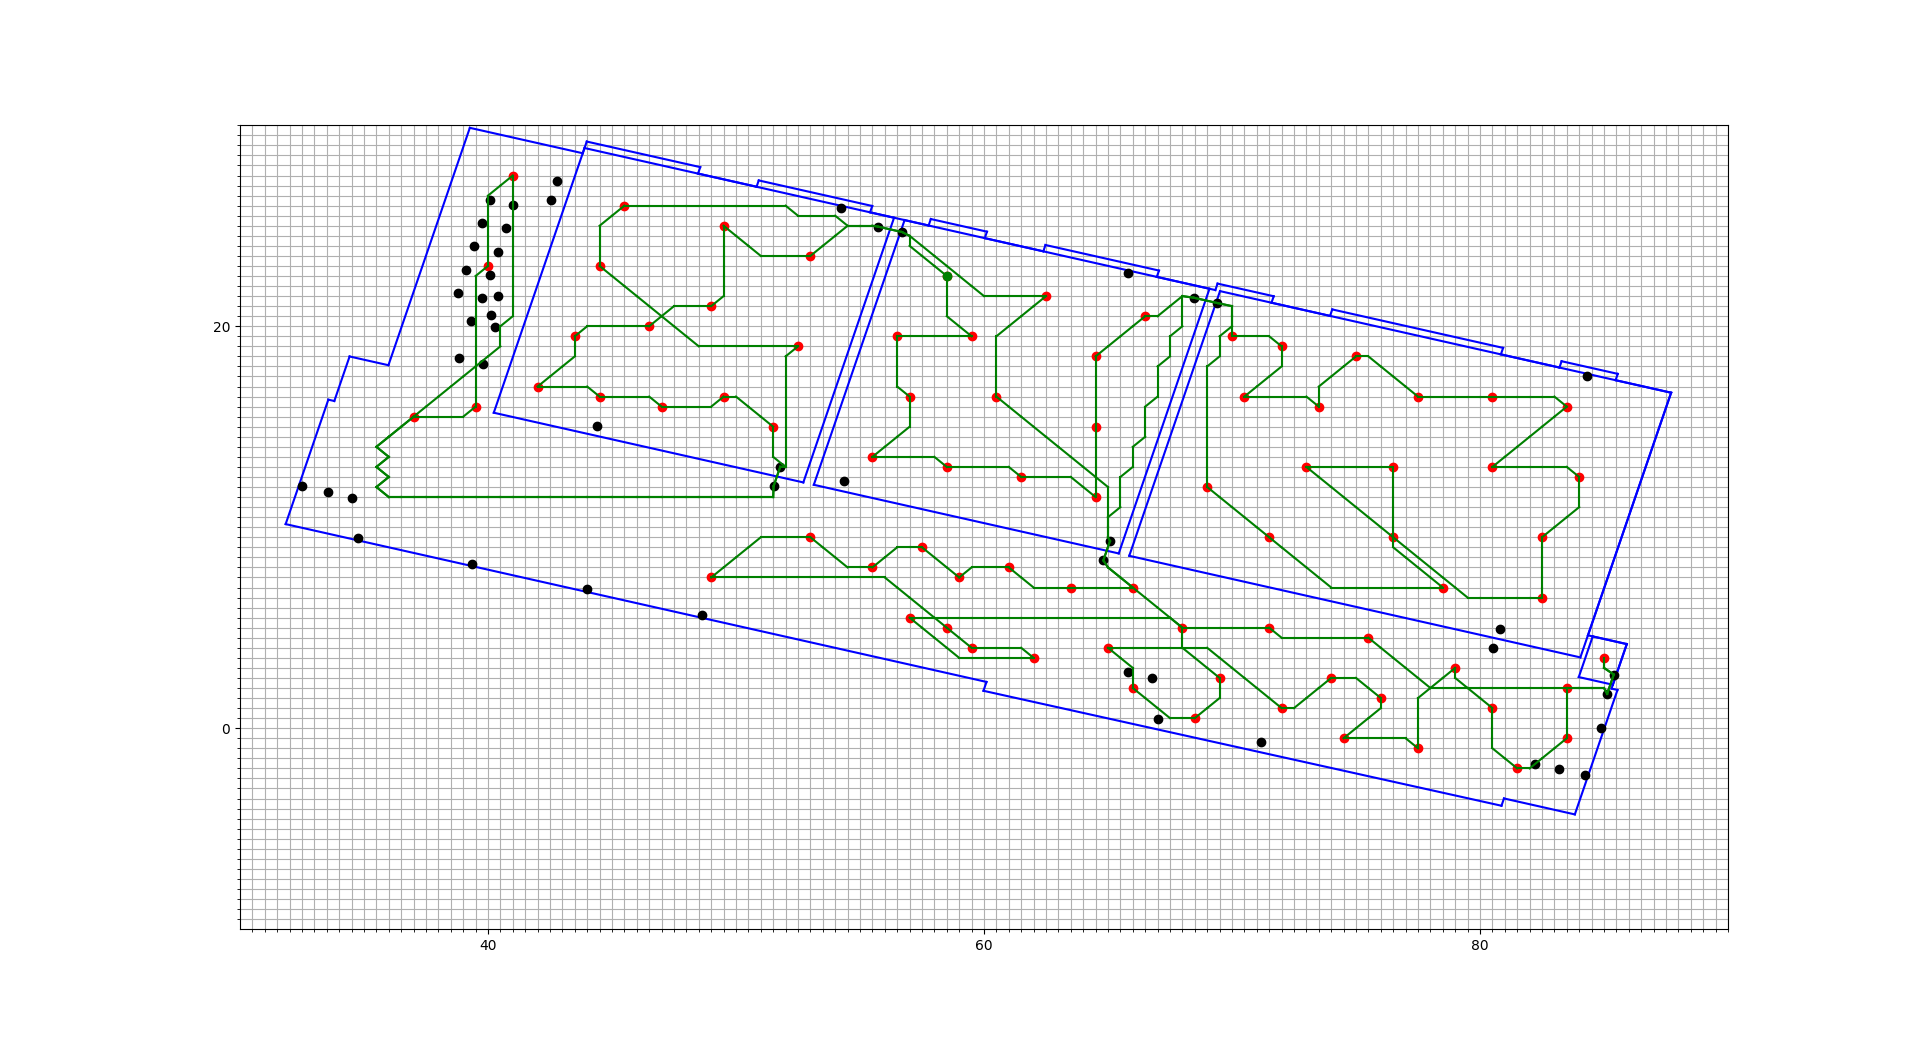
\includegraphics[width=1\textwidth]{fig/Resultater/127/0.31_min_height_radius0.1.png}
    \label{Rum knudepu}
    \caption[Design overview]{}
\end{figure}

\begin{figure}[H]
    \centering
    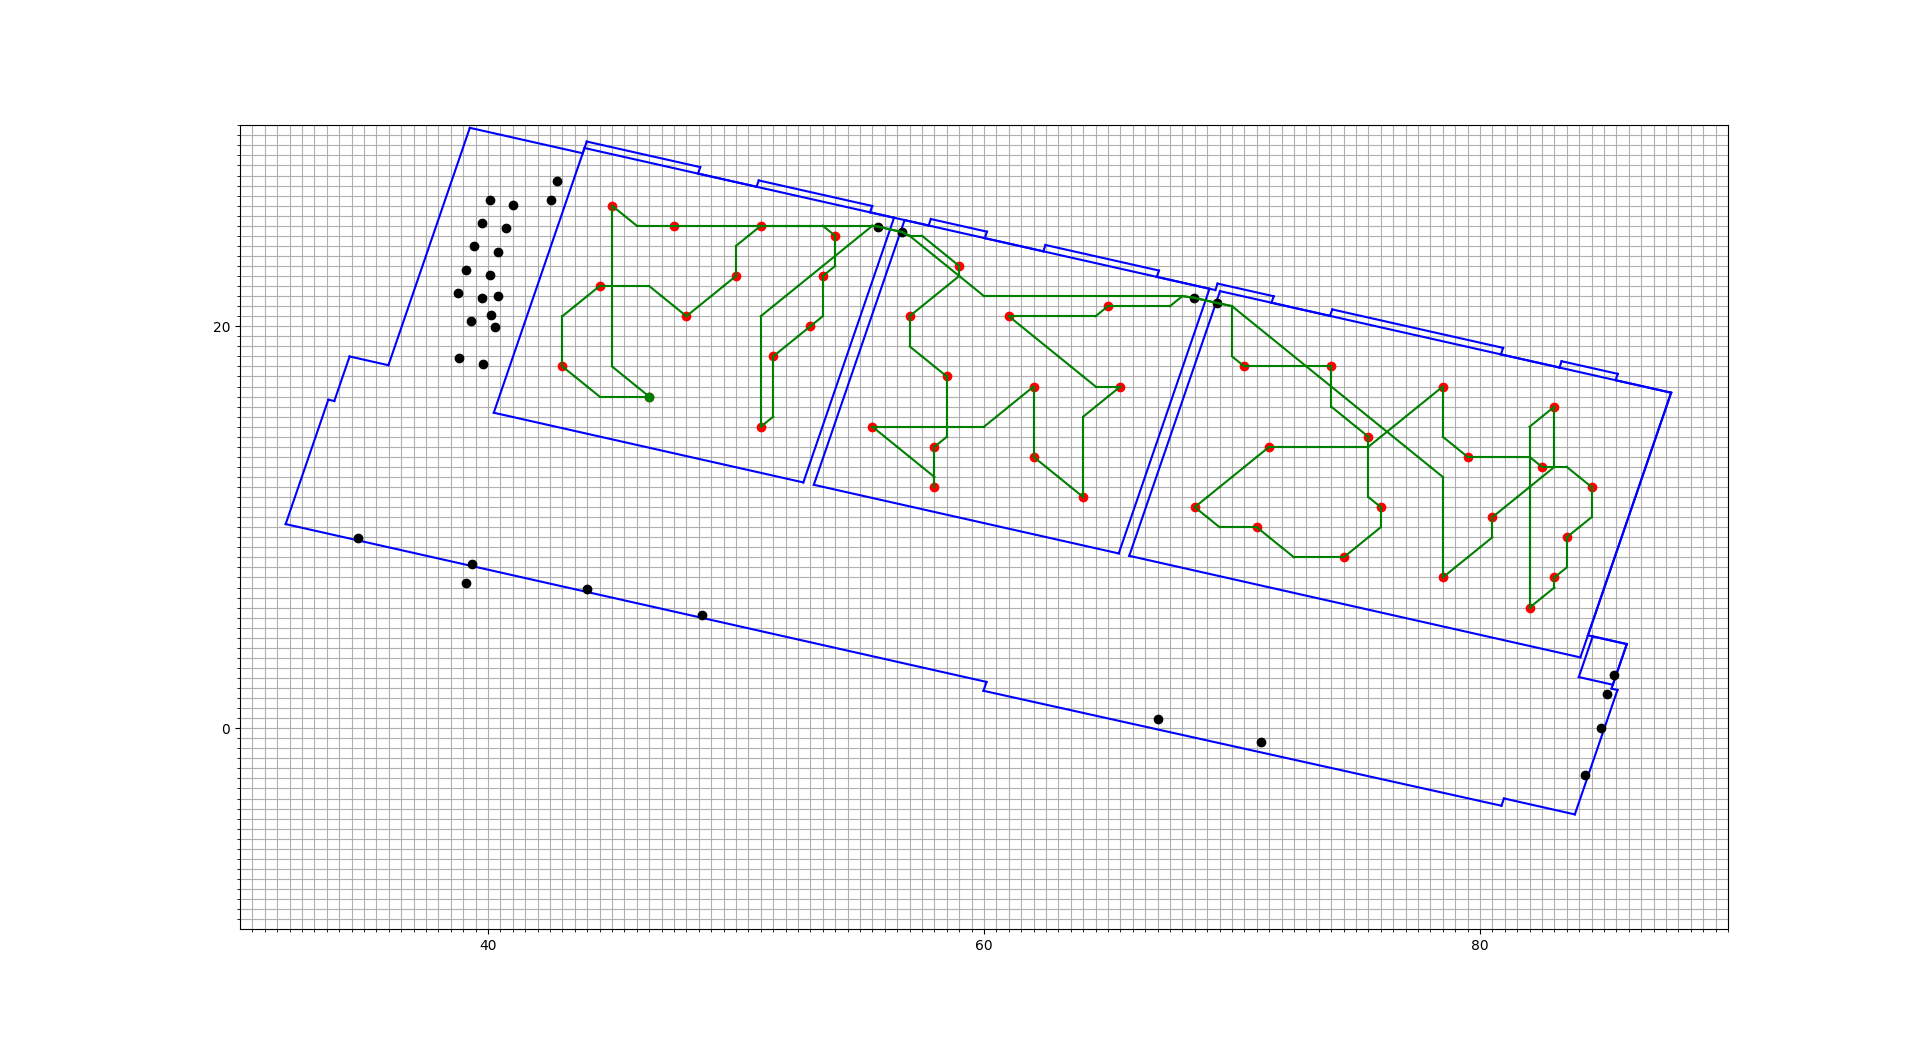
\includegraphics[width=1\textwidth]{fig/Resultater/127/0.31_min_height_radius0.01.png}
    \label{Rum knudepu}
    \caption[Design overview]{}
\end{figure}

on another floor
\begin{figure}[H]
    \centering
    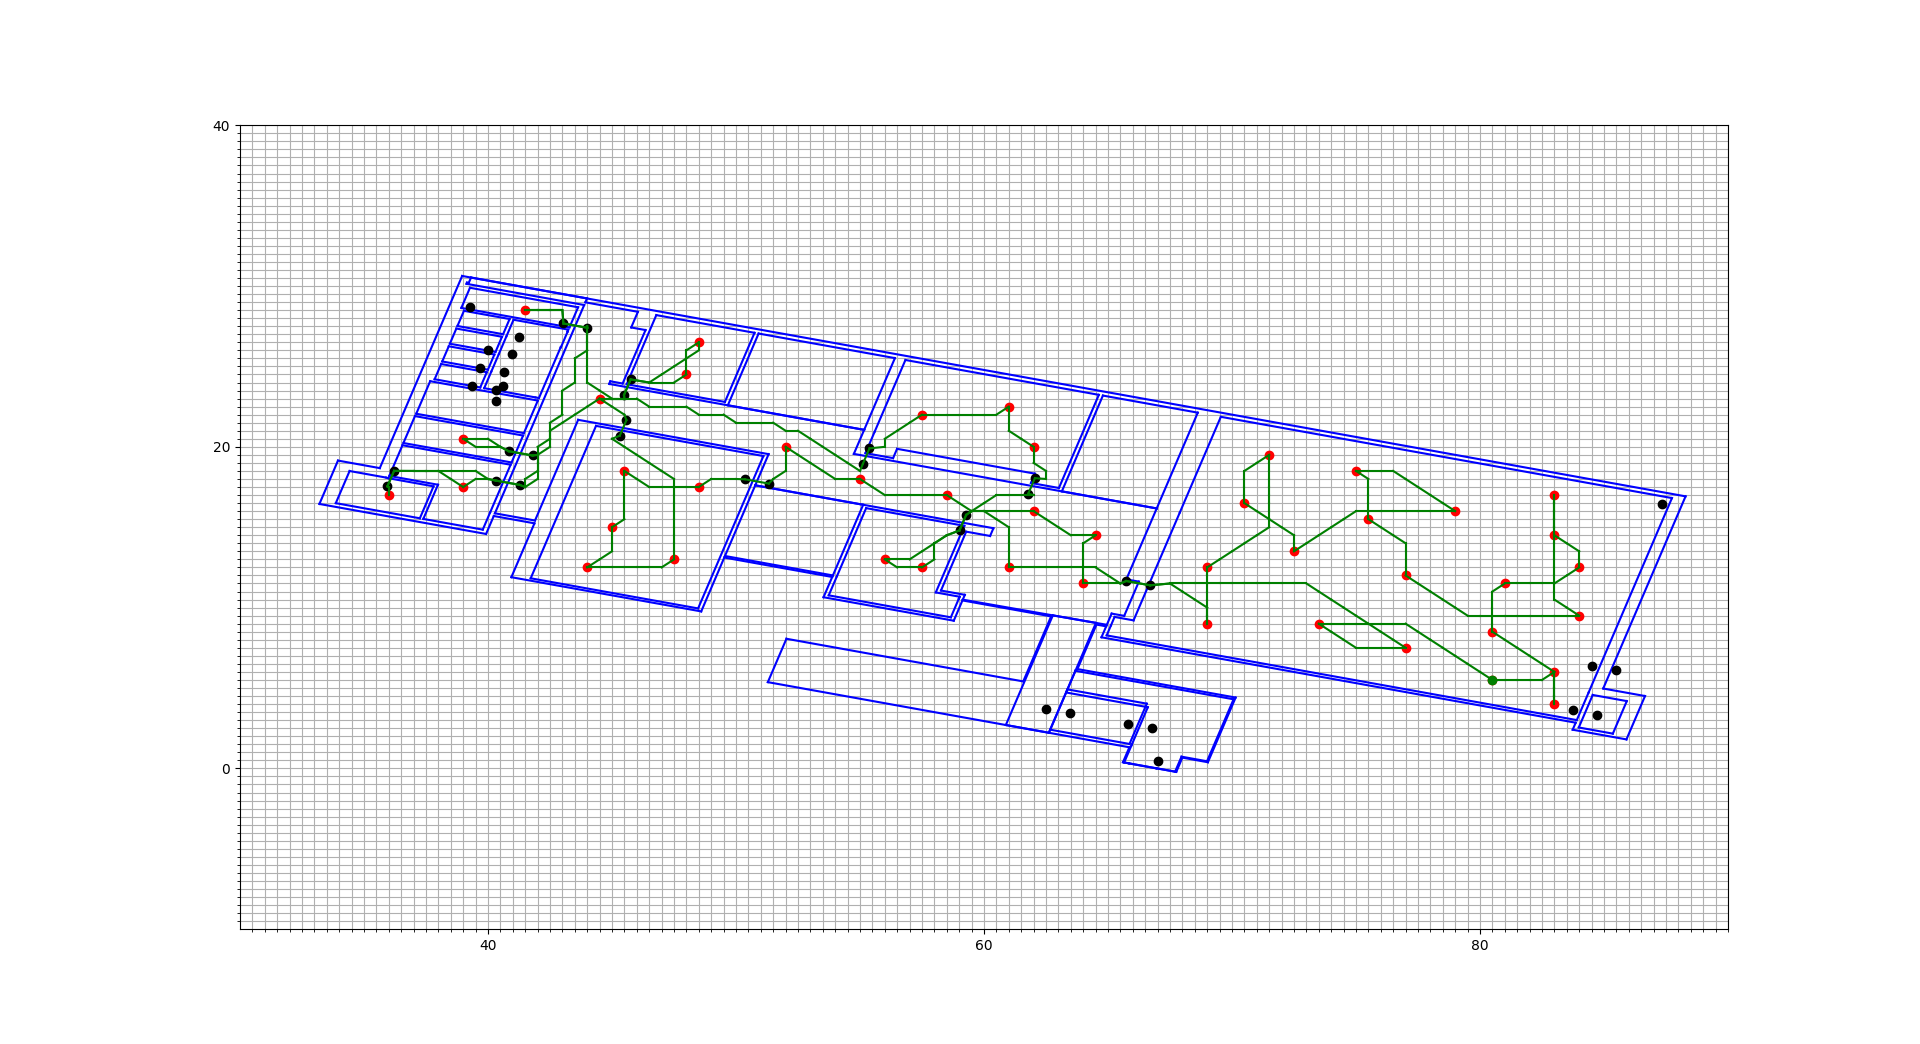
\includegraphics[width=1\textwidth]{fig/Resultater/127/5.36_min_height_radius1.png}
    \label{Rum knudepu}
    \caption[Design overview]{}
\end{figure}
\begin{figure}[H]
    \centering
    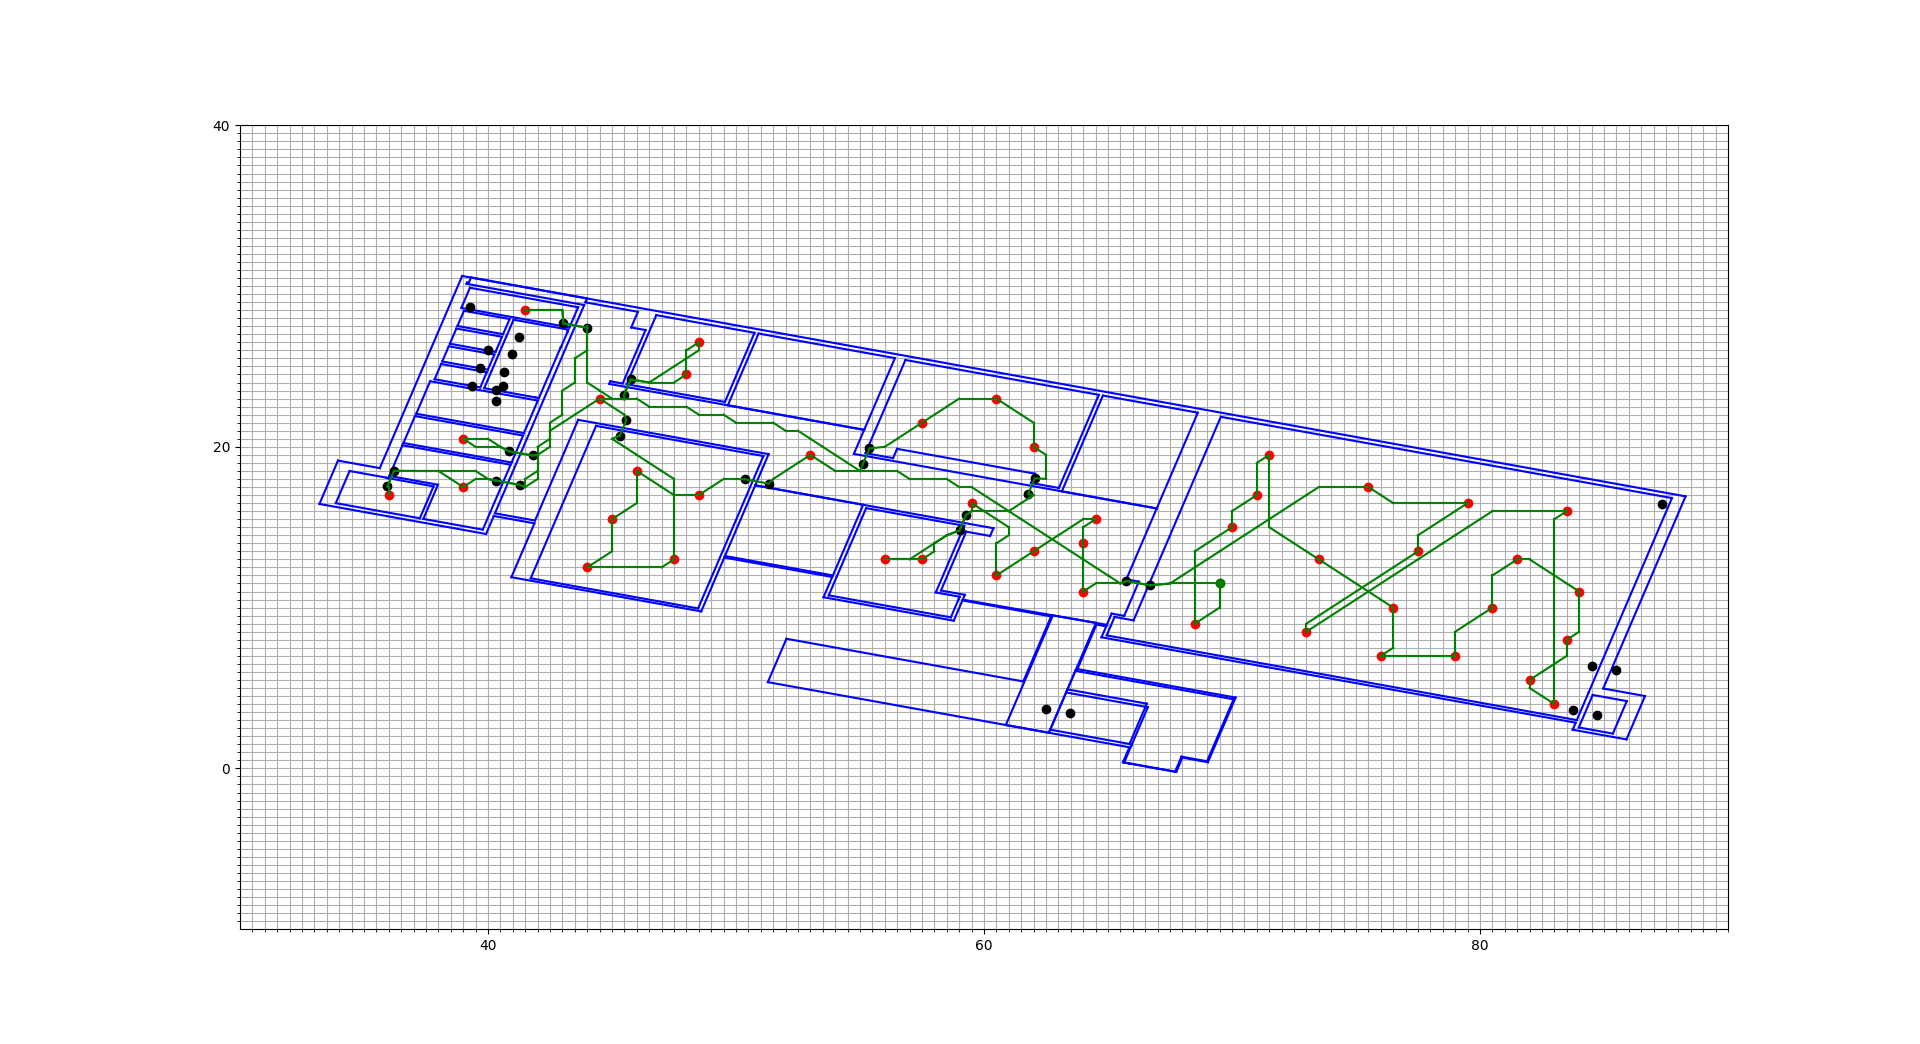
\includegraphics[width=1\textwidth]{fig/Resultater/127/5.36_min_height_radius0.1.png}
    \label{Rum knudepu}
    \caption[Design overview]{}
\end{figure}
\begin{figure}[H]
    \centering
    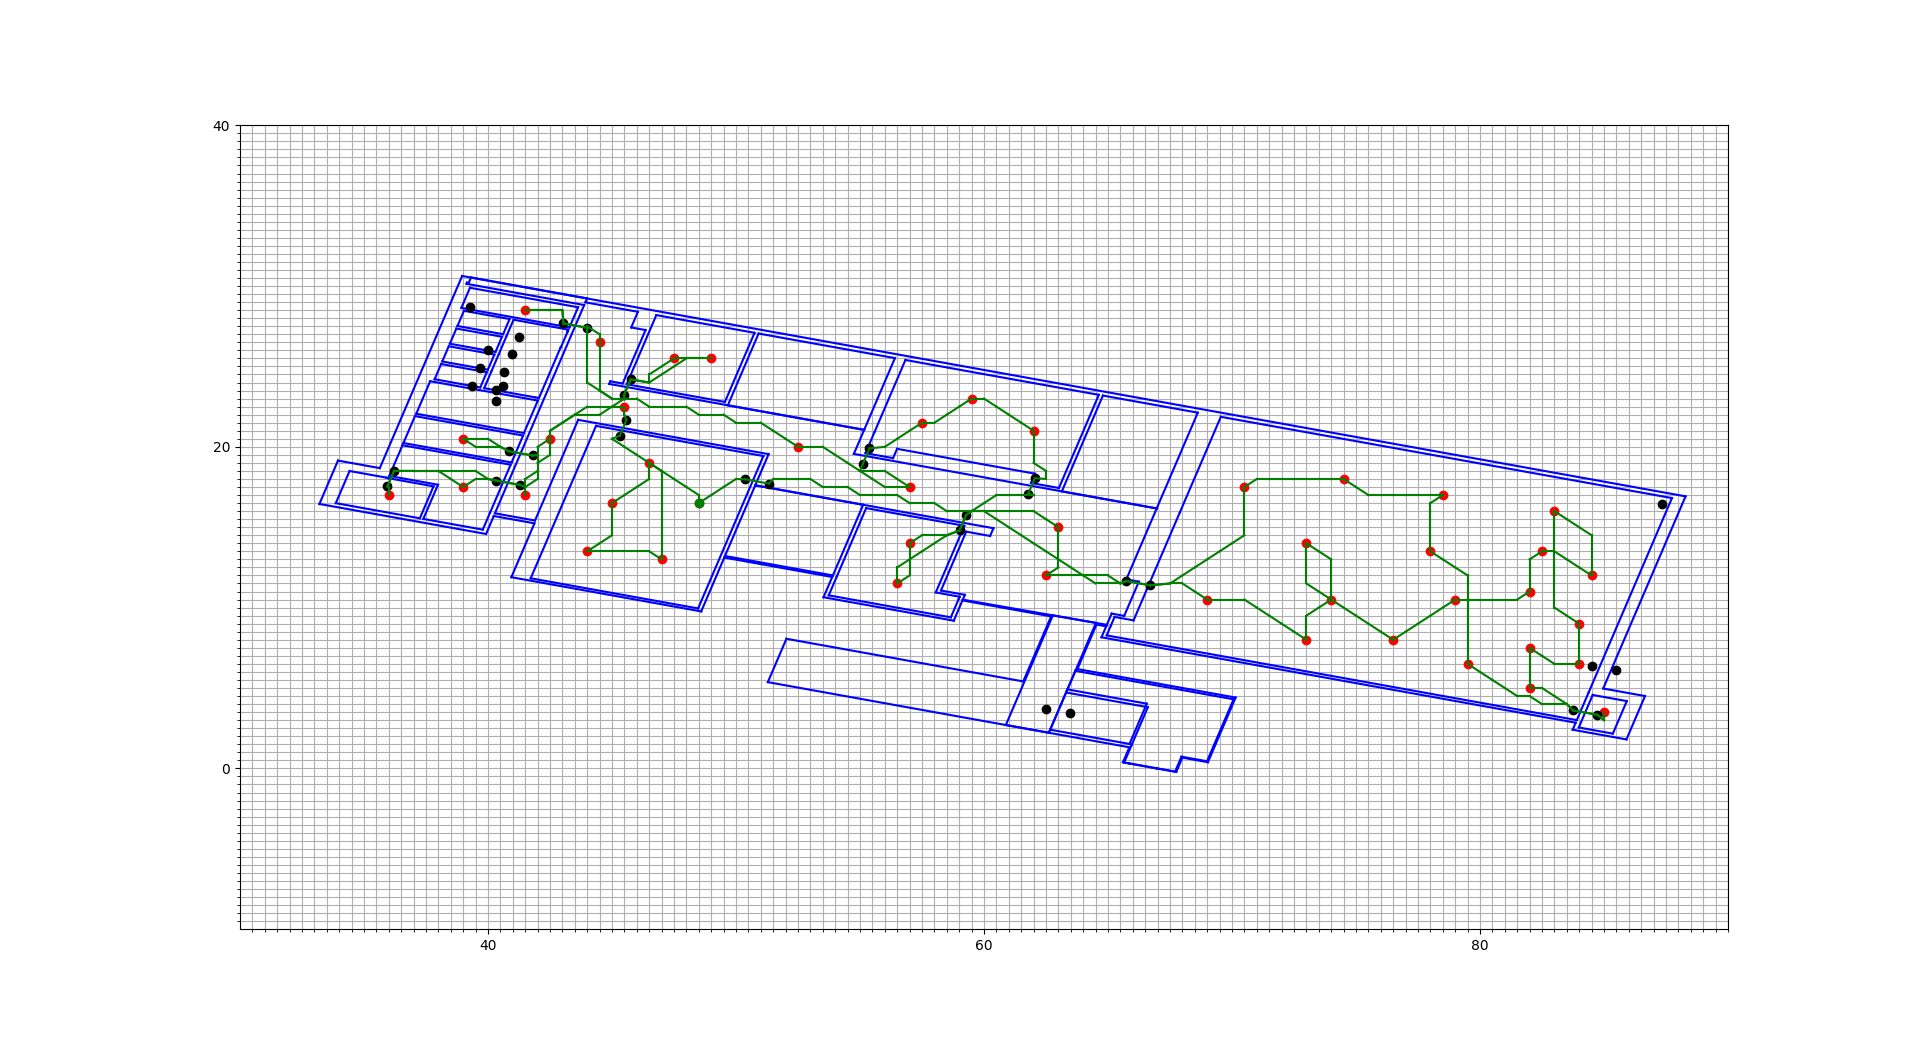
\includegraphics[width=1\textwidth]{fig/Resultater/127/5.36_min_height_radius0.01.png}
    \label{Rum knudepu}
    \caption[Design overview]{}
\end{figure}

Another floor again
Here there is not difference between using 0.01 radius or using 
\begin{figure}[H]
    \centering
    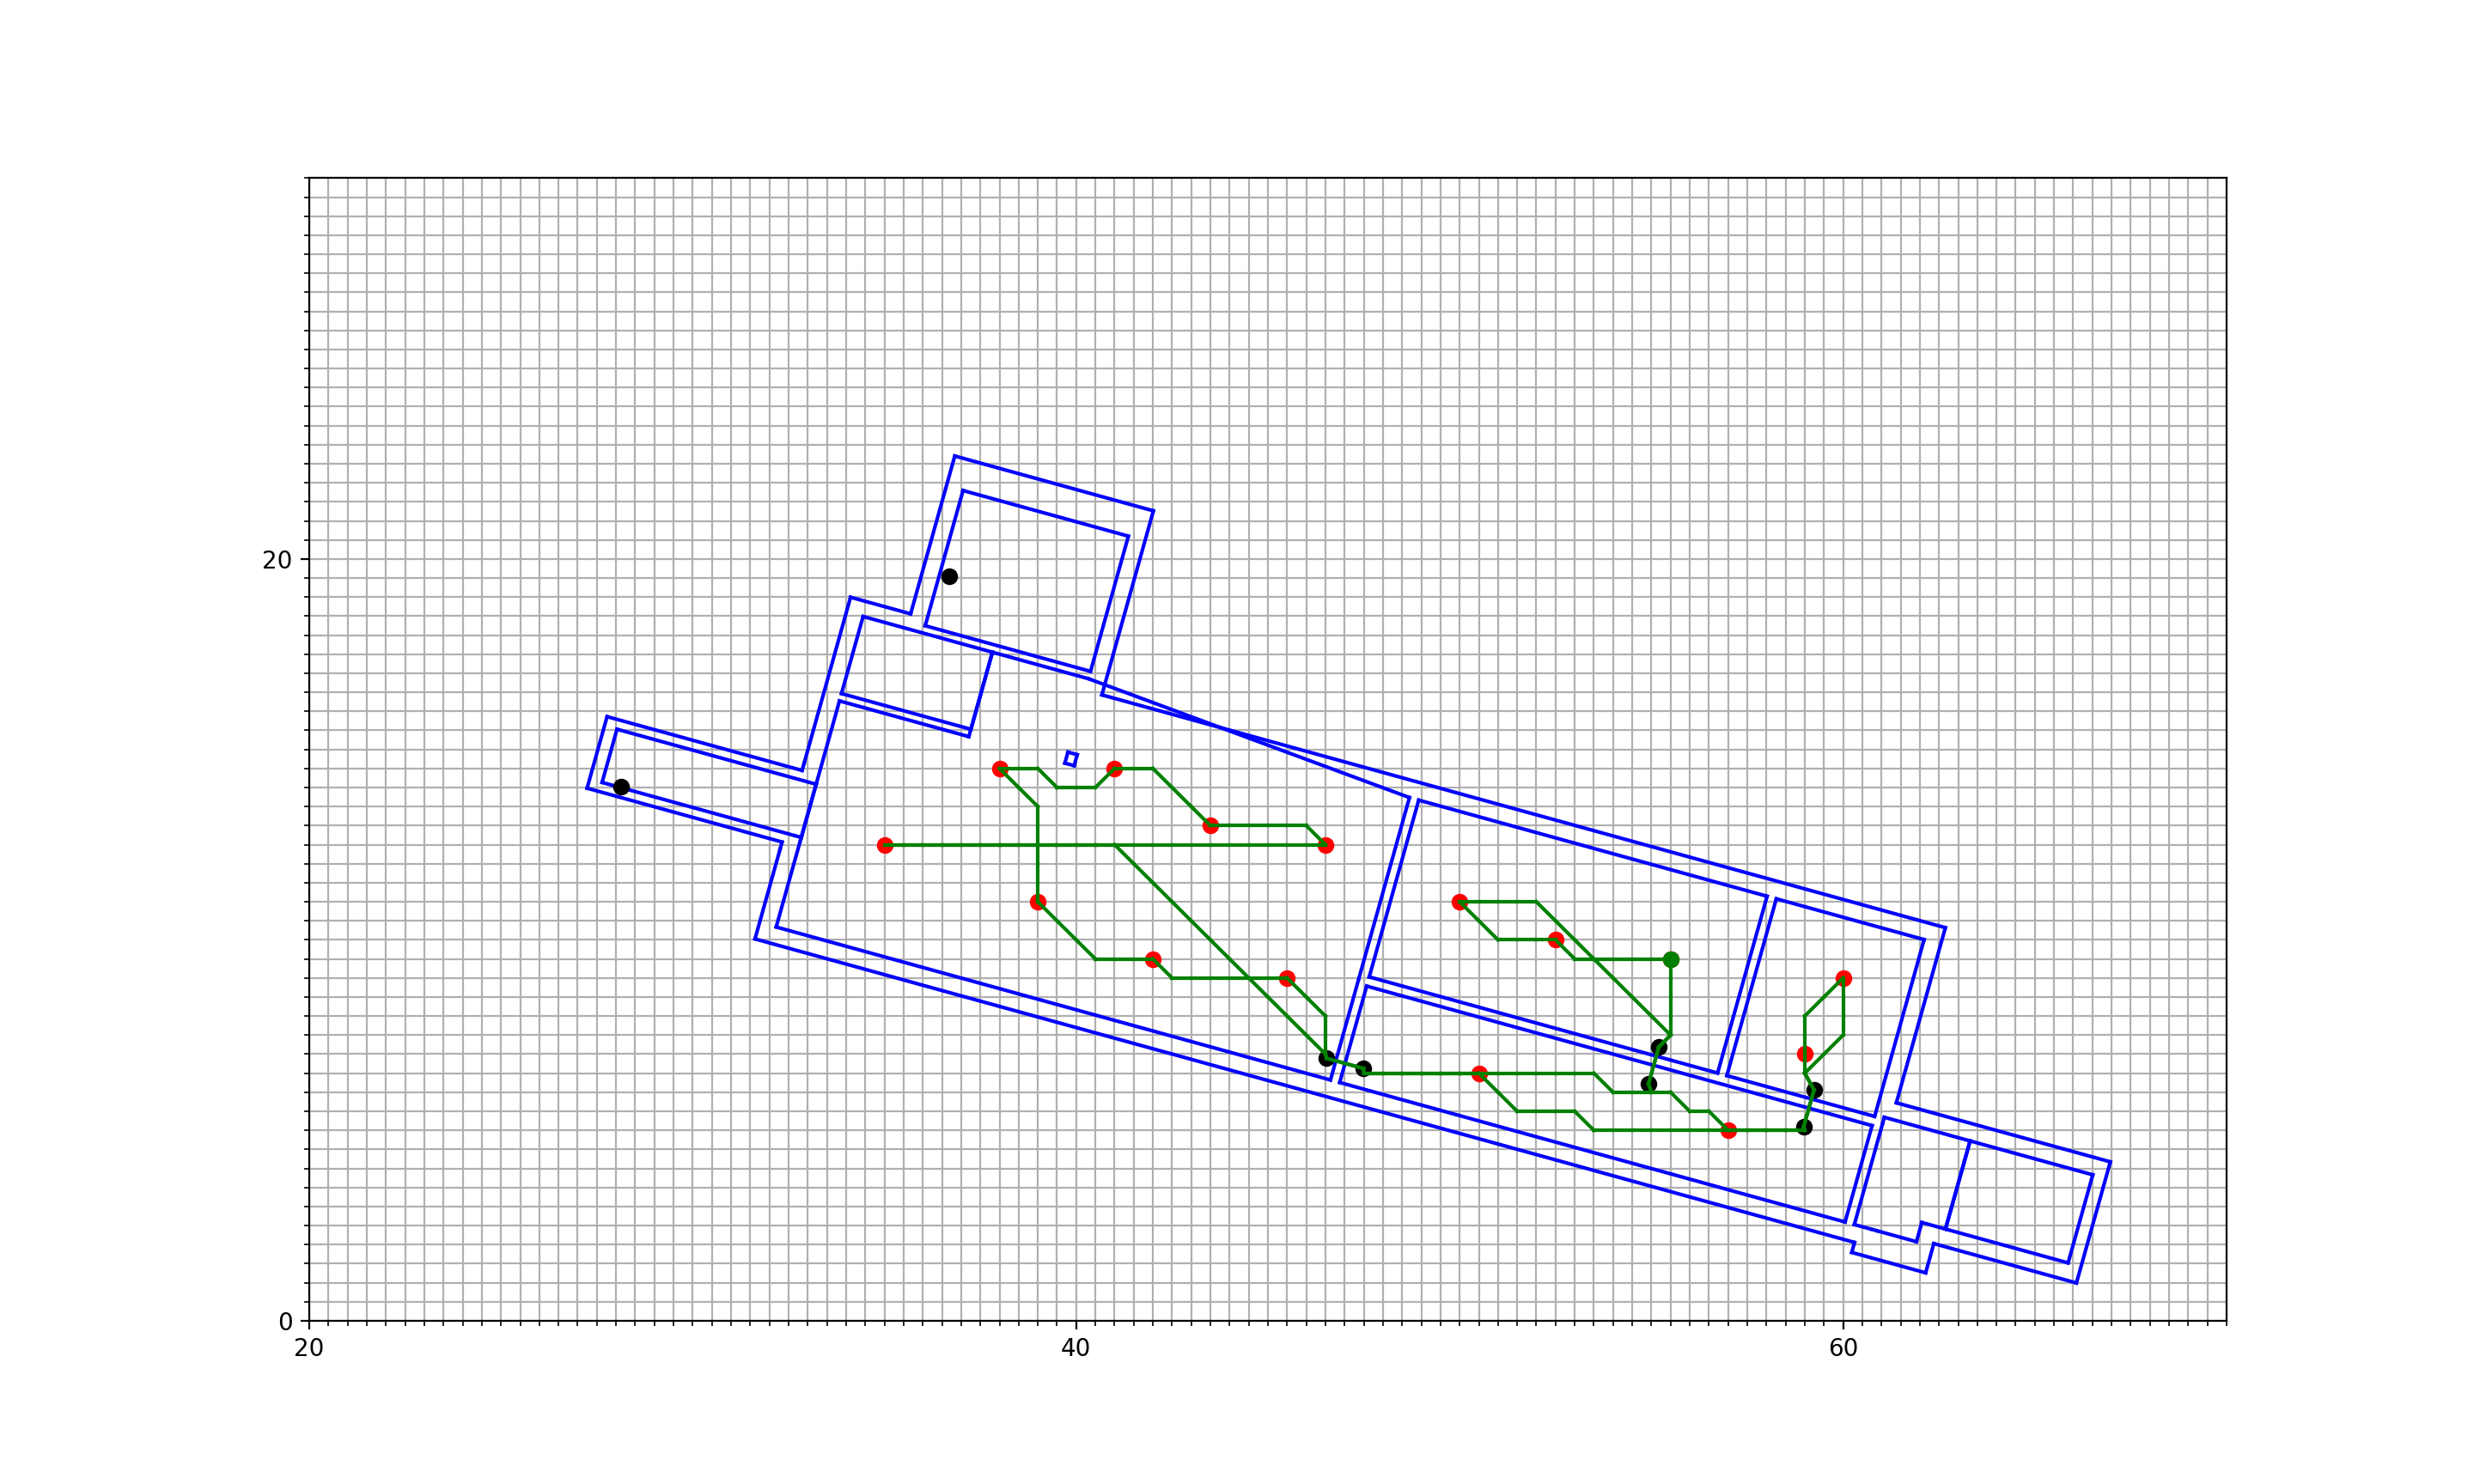
\includegraphics[width=1\textwidth]{fig/Resultater/127/-3.43_min_height.png}
    \label{Rum knudepu}
    \caption[Design overview]{}
\end{figure}
\newpage
\chapter{Discussion}
\section{Results}


\section*{Discussion}
(Comment on your results, explain what those results mean, interpret the results in a wider context. Also indicate which results were expected or unexpected, and provide an explanation for the unexpected results)

\begin{comment}


\subsection{Grid vs graph connectivity}
Explain
\begin{itemize}
    \item both methods 
    \item that the graph doesn't work on weird buildings but grid system does.
    \item That grid scales badly with building size but graph doesn't
    \item f
    \item f
    \item f
    \item Maybe variation in node sizes help
    \item That the robot needs a certain node size to work properly. It doesn't work on nodes in the $mm^2$ range.
\end{itemize}


To make the robot walk from one room to another or one place in the building to another, it is important to understand the and decide on a way to implement the connectivity between the rooms. There are mainly two different kinds of implementations; a graph connectivity implementation and a grid implementation.
\\\\
The grid implementation works by discretizing the floor of the building into a grid with nodes of a specific size; the smaller the node size the higher the resolution of the grid.
\\
The graph connectivity approach works by representing each room/area by a node/dot which will be connected by a line to other rooms in the floor.

The different implementations have different advantages and limitations. For example computationally the graph connectivity approach is much more scalable with bigger buildings or construction sites where as implementing a grid system in these situations will be more taxing computationally since a lot of nodes will have to be calculated. 

On the other hand the advantage of the grid method is that its pathfinding algorithms will work on all building shapes. 
Imagine the floor plan of the building below:


\begin{figure}[H]
    \centering
    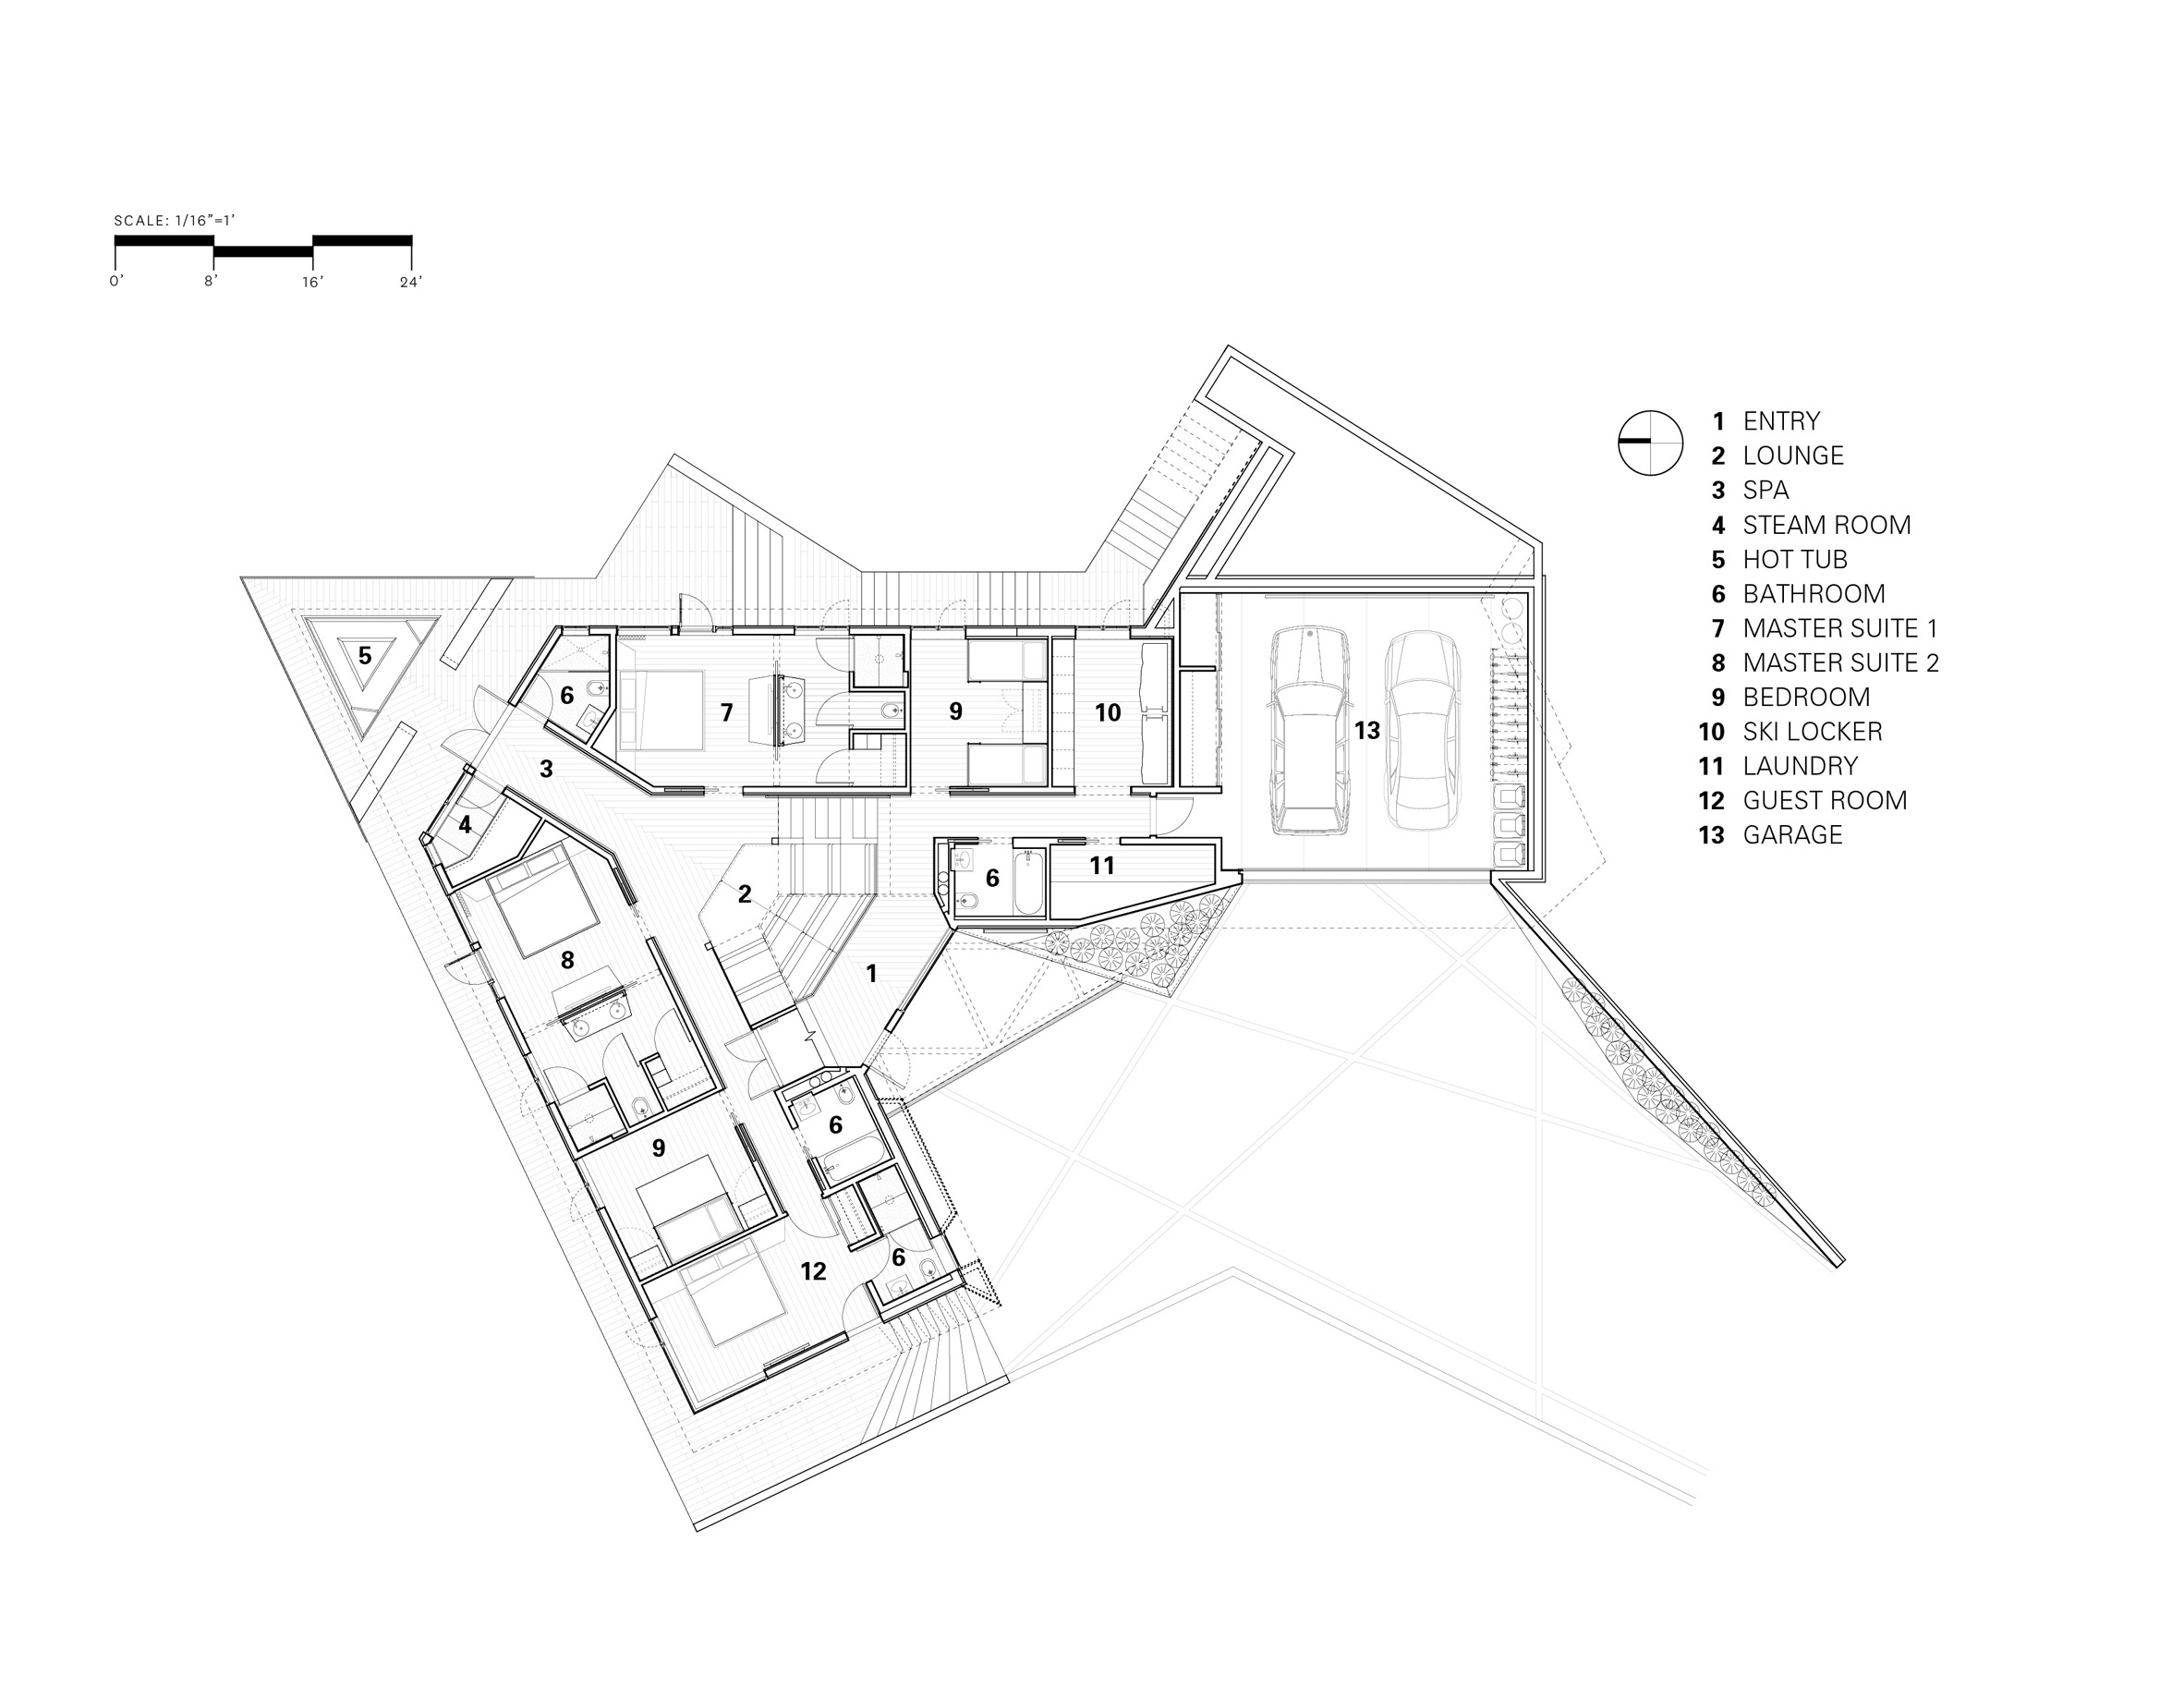
\includegraphics[width=1\textwidth]{fig/weird_floorplan.png}
    \label{}
    \caption[Weird floor plan]{Weird floor plan~\cite{weird_building}}
\end{figure}

When using a grid system apporach it will be possible to get an agent to walk from area 12 to 13 by specifically telling it which nodes are walkable and which nodes are not e.g walls. This will not be possible for the graph connectivity graph. The graph will here see only that area 12 and 13 are connected but not in which way. The method will draw a straight line between the two points and not see that the areas in reality are connected by the long pathway that goes through the entire floor plan.


\subsection{Grid system paper}
In this paper \cite{xu2017bim} they have the goal of solving “Accurate and efficient indoor path planning” in BIM models. The way they have implemented it is by using the grid system. 

\begin{figure}[H]
    \centering
    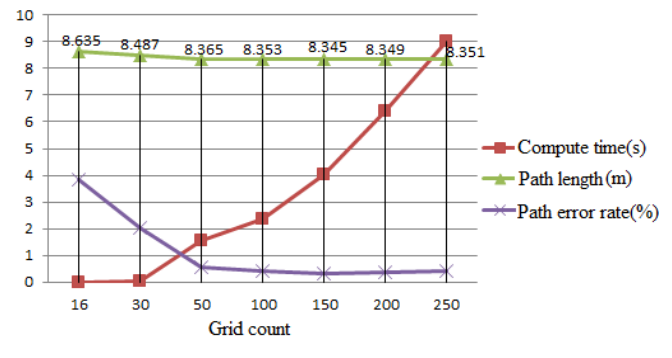
\includegraphics[width=1\textwidth]{fig/graph_grid_system.PNG}
    \caption{Graph showing computation cost as a function of grid count~\cite{xu2017bim}}
    \label{}
\end{figure}

They show what happens with the computation time when increasing the number of nodes. And also shows how minimal an effect it has on the path length.

Skriv om Convex decomposition vs alternativer(K means)

\\\\
\subsection{Conclusion}
blabal


\subsection{Future work}
You can write about slam
Write about stairs
Write about the whole thing about actually getting the robot to traverse the route and programming the robot
\end{comment}

%\newpage
%\section*{Appendix}
\subsection*{My process}
\begin{itemize}
    \item I spent a week or 2 to create the floor plan in python. I then got stuck with the doors since they do not match in any sort of way.
    \item I moved on to experimenting with unity. Making a grid system that could implement A*.
    \item I spent time researching whether to use the grid system or the graph/polygonal system.
    \item I went back to trying to find the best software for simulation in the future also.
    \item Now I am back to implementing the algorithm in python 2D like they did in the 3 week report, before doing the simulation in unity.
    \item I implemented the TSP solution to the problem. 
    \item I visited the Spot robot in Odense
\end{itemize}

\subsection*{General questions to answer}
\begin{itemize}
    \item How to get around the building
    \item How to get from room to room/around the building in an appropriate way?
\end{itemize}
%\section{Code notes}

\subsection{#1}
This is a function called dict_hashing. The purpose of this function is to hash the lines.

\subsection{Plotting rooms}
In this section we plot the floorplan outline and the rooms within it. We start by doing some simple preprocessing of the csv file with the rooms. 
The number of coordinates of each room is always dividable by 3 since it is created in such a way that each room is spanned by sets of triangles - hence it takes 3 coordinates to make up a triangle.

For each triangle we hash all lines in that triangle in a dictionary in both direction. This means that we hash 6 lines per triangle. The reason for this is that a triangle might have the same line as another triangle but in reverse order. These two lines should be seen as the same. Therefore we have to hash both directions of each line in every triangle.

For example say we have a line in one triangle (x1,y1) - (x2,y2). What we do is that we hash the line (x2,y2)-(x1,y1) as well. What happens now is that the other triangle has the same line but as (x2,y2) - (x1,y1). Just like the other triangle both directions will be hashed meaning (x1,y1)-(x2,y2). The way hashing works is that 2 identical values will give the same hash key. In this example we now have 2 values for 2 different hash keys, since the same line is occuring twice in 2 different hashes.

Now each dictionary element that has more than one value is removed. Therefore both of the hashes will be removed and we have made sure that the line is correctly removed.

Some other removal criterias are also present. This include manually removing lines/ walls that clearly are misplaced.

The way we hash also has the consequence of having each line existing twice in the dictionary. Therefore one of the directions of each line is removed. This makes the dictionary half as long and makes is more efficient for use later if need be.

At last we plot each line in the dictionary.
And repeat the process for a new room, setting the dictionary back to empty. The dictionary is concatenated with another dictionary that keeps all the lines of the floorplan for later use.


\subsection{Plotting the doors}
Again the program does some preprocessing on the csv file with the door coordinates. This csv file include the coordinate of each door and the direction it is facing. The last line of the csv consists of the coordinate translation.

For each door - depending on the direction it is facing - another door will be added on the other side of the wall it is facing. This makes it possible to go through doors. The reason for this will be explained in the TSP section.

Each door and its copy is then plotted.

\subsection{Adding room nodes}
The room nodes are the nodes are points of interest that the spot robot should visit. At this point the points are placed manually and arbitrarely. Later some algorithm will be made to place them.

\section{Traveling salesman approximate path}
\subsection{plotting all walkable paths}
The objective here is to for each node have which other nodes it can traverse to. The path between two nodes is not traversable if it is obstructed by a wall. 
An easy way to implement this is using a network datastructure. In this case the networkx framework is used. Nodes are created in the network for all points created - which includes door nodes and room nodes. 
Line intersection is them used to check if two nodes are traversable.
If they are traversable then we add an edge between the two nodes to the network with the weight of the edge being the euclidean distance between the two nodes.


\subsection{Shortest path between all "room" nodes}
The objective here is to find the shortest traversable path between all room nodes. This is usefull when we later want to find the minimum spanningtree and the approximate TSP solutions.

The networkx library has a function that performs dijkstras algorithm. A foor loop is run for each room node.The dijkstra function takes in the Network and a source node and outputs its distance to all other nodes and also the predecessors. The predecessors is for example if there are 4 nodes 1,2,3,4. If 1 and 4 is not directly connected, but are connected via node 2. What will happen is that the distance between 1 and 4 is still calculated in the distance output of the function but the predecessors for 2 will be 1 and for 4 will be 2 (if 1 is the source node).


\subsection{Make complete subgraph of all room nodes}
To use the approximate solutions of the tsp problem, many rely on the assumption of a complete graph. This means that all nodes in the graph are connected. One thing to note is that since we don't wish to find the tsp solution for all nodes (door,corner and room nodes) we wish to make a subgraph of only the room nodes. This graph should also be complete. 

This is done by first making a new graph that only include the room nodes.
We then compute the distance between each node in G_rooms using dijkstras function again.



\subsection{Minimum spanning tree}
This is a one line code that makes a minimum spanning tree given a network. This comes from the networkx framework. 
The minimum spanning tree is needed to do the approximate solution of the tsp problem.


\subsection{Solve TSP problem for subgraph using DFS traversal}
This is again a one line of code, where a depth first search traversal is performed on the minimum spanning tree of the rooms. 

The next step to finalize the tsp solution is to remove double vertices occuring when doing the depth first seach algorithm on the minimum spanning tree.

The dfs list consists of node pairs with a 'from' node and a 'to' node.
e.g
(1,2), (2,3), (3,4) etc.
We can have that the 'from' node of the current node pair is not the 'to' node of the previous node pair. 
e.g
(1,2), (1,3)
When this happens we want to make i a shortcut such that it goes directly from 2 to 3 without going back to one.


We do this by having a for loop that runs through all node pairs in the list of the depth first search edges. 
If the 'to' node in the previous node pair
is not the same as the from node in the next node pair then the new 'from' node should be the previous 'to' node and the new 'to' node
should be the current 'to' node.
For example if we have (1,2), (1,3) then because we go back to 1 we change it to (1,2), (2,3).



\subsection{Time of code snippets}
\begin{center}
\begin{tabular}{ |c|c|c| } 
 \hline
 Code snippet & min time & max time \\ 
 Reading room and door data and plotting the room (without plt.show) & 0.3 & 0.8 \\ 
 Plotting the grid & 0.002 & 0.003 \\
 appending points in grid & 0.04 & 0.04 \\
 \hline
\end{tabular}
\end{center}


Calculating distance to the nearest wall for different amount of grid points - time.
The total amount of grid points is 15207 
\begin{center}
\begin{tabular}{ |c|c|c| } 
 \hline
 Grid points& min time & max time \\ 
 10 & 0.009 & 0 \\ 
 100 & 0.09 & 0 \\
 1000 & 3.35 & 0 \\
 2000 & 11.8 & 0 \\
 3000 & 23.9 &
 \hline
\end{tabular}
\end{center}












\subsection{#10}
%\section{Noter}
\section{Spørgsmål til vejledere}
Software design and architecture for the code?
Sketching by hand?
Focus on refactoring? Struktureret og læsbar.
Spørg om du skal skrive at du brugte meget energi på at hoppe rundt fra platform til platform og fra diskret til ikke diskret implementeringer.
Is there a problem with the resolution of the plots?
Skal den stå stille mens den tager en punkt sky eller kan den gøre det mens den er i bevægelse, spørg evt Anders?
Spørg andreas og Jeppe om den generelle struktur af din rapport og de sektioner du gerne vil snakke om.
Er headline for sektionerne i metode afsnittet, de metoder jeg har brugt eller de problemer jeg har løst? Hvad er det væsentlige at snakke om. 
F.eks. problemet med room labels bruger man metoden winding number. I analyse delen har jeg så beskrevet winding number lidt.
Jeg har spurgt om det før, men jeg bruger "we" for at skrive i aktiv form.
Jeg har svært ved at vurdere om de forskellige sektioner skal være i metode afsnittet eller i implementations afsnittet, f.eks. sampling graph afsnittet.
Min udfordring er at lave denne røde tråd i metode og implementeringsafsnittet. Mange af de ting jeg gør er implementering hvor jeg ikke bruger en specifik metode. Jeg kunne godt overveje at man i metode afsnittet havde metoderne som headlines og i implementation forklarer hvordan man implementeret hele programmet. Jeg har svært ved at vurdere hvad der er vigtige og ikke vigtige implementeringsdetaljer..
Jeg har læst lidt videre omkring passiv og active form fordi det er meget svært at skrive i aktiv form uden at bruge nogle pronomener, som "we" for eksempel, det er svært at bruge programmet som subjektet.
 
\subsection{Thesis noter}
Explain the fundamental problems which will be the background of your theses.
Maybe build it up as a story.
Say not what you are going to do but why.
Start with the why. Elevator pitch in the first section.
Remember that you are writing with human beings. Have a good flow. Have 1.5 months for report writing.
Nudge people into the topic and not straight into it.

Related works doesn't have to be detailed.
Theory of the things you use is background
Present papers in related work, provide an overview of the theories briefly.
Background is only theory on what you have implemented.
Related might be after background.
More than 5 references, have as many as possible.
How long the report, write more background if bad contribution, more report.
The reader should not have a burning question.
Be very explicit about the scope of the report.What will you not go into.

Method is about what you have done yourself, no matter what you have followed, make proper citation 
You can also have a little introduction paragraph, saying you are following this method.
Have implementation section, the tools, the computer used.

How to show the results?
How to make results?
What results could you present that support that you finished the project.
Google sheets

All the time consider getting credit for what you did
Get more credit by discussing the way you got there. Some of the considerations you made and the issues you solved.
Explain how you ended up with the final product and why?
By extending the method section.

We can get a quick readthrough of the report but not a detailed read

General rule is that the citation should not be as nouns.
Use the name of the reference, and then cite.
Write the name of author and the year not the name of the paper. Typically.
How much in appendix all code or just link to github?
Rule of thump have small code snippets in the actual report if it is important. It is fine in the appendix just have the link to the github repository.

30 min presentation
15 min spm 
Fremlæg om oversigt over dit projekt
Introducer projektet og motiver det
Forklaring af metode
Vis nogle af resultaterne 
Du kan bruge resultaterne til at beskrive metoden.
Du kan godt flette de to ting sammen.
oversigt
Husk at have afhandlingen med i pdf
Forbered slides til spørgsmål du tror vil komme.
Hvilke regler i forhold til regler? 

analyse,design og implementering i software projekter.
Analyse: Hvad har du til rådighed?
Hvad kan jeg bruge til at forbedre på det.

implementering: kode og algorithmer. Mest bare for vigtige detaljer omkring hvordan du har implementeret ting.

As stated in [McAuthorson, 1989] foo is bar. Dette er den bedste måde at gøre det på.


Generaliser lidt ud over Dalux, så det ikke tager udgangspunkt i Dalux.
Formuler nogle punkter med antagelser for den floorplan. 
En liste med krav jeg stiller for at programmet kan håndtere det.


Det er meget vigtigt for din rapport at du får skilt problem stillingerne ad, evt. skriv en mail til andreas hvor han kan uddybe det på skrift.

Jeg tænker det umiddelbart som om at du skal lave en skilning mellem at det at tegne figuren og datastrukturen og graph theorien der ligger bag. 


Få akademiske citater er et problem, akademiske reference er vigtige og man taber point på det.

Heller noget i rapporten som ikke er perfekt, men du kan stadig få lidt kredit for det. Skønhedsfejl er okay

I rapporten skal du gøre klart hvordan du har ændret cad tegningen. Du behøver ikke bruge alt for meget energi på det nu. Det er ikke et interessant problem.
Man kan ændre problemstillingen så den passer med resultatet.
inledning er godt have synosis.
Software projekt. Indledning,  Analyse,  design, implemantation

Analyse: Hvis jeg skal løse problemet med noget software, hvad kan jeg så finde i litteraturen og forskellige værktøjer.
Design: Forklar hvordan softwaret skal designes for at løse 
Implementation: Detaljer om implementation

Software der kan løse problemet analyserer værktøjer, 
design: ud fra analysen forklar hvordan software skal designes 
implementation: detalje omkring implementation.
Test, resultat. Diskussion og konklusion.

ANALYTISK og ikke syntetisk i tilgang.
Det er ikke en log, hovedpersonen er problemet du skal løse, du skal angribe det som en detektiv. 

Man får mere credit af at gøre få ting grundigt istedet for mange ting rodet. 
Projekt planen skal være dynamisk.
relatere oprindelig plan til hvad der skete, appendix med arbejdsprocessen.

Hvad er cad modeller og robotten.
Giv en kontekst.
Hvorfor er vi interesseret i at løse problemet.
Ikke dokumentation af programmet. Censor vil i dette tilfælde ikke forstå hvorfor du gør hvad du gør.
Gør det hele til en samlet historie, rød tråd og fremhæve hvor du har fundet gode løsninger.
Du er ikke hovedpersonen, problemet er hovedpersonen. 
Beskriv erfaringerne som en detektivhistorie. 
Sporene i historien.
At lægge en analyse frem.
Hvad skal jeg prøve på løse og hvorfor -> Hvad har jeg til at løse det -> Hvad er så de rigtige løsninger.
Det kan godt være det kommer i en anden tidslig rækkefølge end det du har gjort. 

\subsection{Noter til Paper}
Trying to solve “Accurate and efficient indoor path planning” since a lot of 
people uses indoor walking. There are challenges with indoor navigation.
\\\\
Industry Foundation Classes (IFC)
Semantic information in BIM models
Revit
Triangular prism subdivision
Geometric and semantic information
2D grid subdivision and 3D space subdivision based on triangular prism.
How about if you use variable sizes of grid, depending on the rooms.


\subsection{Noter til master these: Pathfinding in Two-dimensional
Worlds }

You can represent the 2D world in 2 ways, as a 8-grid system and a polygonal way. 
The problems with the grid system are suboptimal path length and the problem of choosing a fitting grid resolution.

Polygons works by connecting each portruding corner and making a connection graph.

A* works on graphs and grids
JPS (jump point search) works on grids only, and is good for large areas of open space.

HPA is also a good algorithm for grid systems but is not necessarily optimal. At most 1\% worse than optimal. 
Makes use of preprocessing, and clusters the map and makes a graph of higher abstractions such that it gets an overview 
of the overall structure of the map before doing the pathfinding.
A fitting cluster size is also of importance for HPA* as we saw in the Scaled Maze map.

VG (visibility graph)
is an algorithm that works on polygonal maps.



\subsection{Noter process og generelle tanker}
\subsubsection{Rapport tanker}
Rapporten består af undersøgende arbejde og er vigtigere end implementationen.
Rapport bliver vurderet på diskussion.
Man kan gøre det på mange måder.
Ulempen ved connectivitet er at man ikke kan se væggene. Graph måden.
Find så mange metoder som muligt og skriv hvorfor de andre er dårlige.
Det viser at du har tænkt dig.
Rapport stuff: for og imod forskellige implementationer.
Kriterie liste med fordele og ulemper.
Undersøg begge veje, og argumenter.
Undersøg på papir og læs dig frem til det. Skriv for og imod for begge.
Læs en masse artikler, og skriv alle tanker omkring det.

\subsubsection{Ugentlige rapporter}
Hvad skete I den forgangne uge, hvad har været nogle problemer.
Ugerapport der beskriver status.
Skriv nogle noter til jer selv.
Små tekst stumper
Trello planlægning, to do liste
Include figures and bibtex and notes.


\subsubsection{Brainstorm}
Lav en meget præcis liste med ting du skal have gjort så du altid har noget at lave.
Brug en time på det i to doist.

Hvad skal jeg gøre i sidste ende?
Robotten skal kunne bevæge sig fra punkt til punkt i en bygning mens den tager billeder på en etage. Den skal have en strategi til hvordan den går rundt og hvordan den undviger forhindringer.

En meget overordnet planlægning af hvordan du kommer systematisk rundt i en bygning, så den kan blive scannet.
Denne opgave behøver ikke være så geometrisk. Du kan egentlig se en bygning som en graf, hvor hver knude svarer til et rum.

Det andet element er at komme rundt i de enkelte rum og gå fra rum til rum på en hensigtsmæssig måde.
How to compare different methods?

\section{Svar på spm}
\subsection{Skal jeg skrive i passiv eller aktiv form?}
The project is being worked on in collaboration with...
I am working on the project in collaboration with…
\\\\
Brug aktiv form. En gang på siden bruge “I”.
Som regel inkluderer man læseren og bruger “We”, hvis det er noget du har lavet så “I”.
Tit bruger man ikke personer som subjekt.
Brug mest aktiv, der må gerne være lidt passivt.


Gulv areal hvert pixel bliver et grid punk. Skyd en email hvis du løbetr ind i problemer.
Unity reflect det der oversætter bim modeller til unity. Hen ad vejen måske.
Ray trace bim model der kunen hjælpe med at finde ud af fra et punkt til et andet.



\subsection{Uge 7}
Figure out exactly whats going on with data.
It seems that it is mixing up axis.
Switching x,y for the doors
RAC look into the building 
Study the format and file
send code and description to andreas, also useful for report.

What I want to do is to remove all doors that are not connected to a wall. To do this I am going to find the distance for each point to all the walls (might change this to closest walls). Since I only have the coordinates and not the lines what I am going to do is to make a triangle including the two points of the line and the third point being the door node. I am going to find the length of each side of the triangle. Using Herons formula I will find the area, and knowing the area I will find the height of the triangle. The only issue is that the distance from the point to the line is not always equal the height of the triangle. The distance could be longer - not shorter though.

Sagen er den at RAC bygningen er ikke en bygning der eksisterer i virkeligheden (ihvertfald ikke I Danmark). Jeg har fundet 3D modellen af bygningen, hvor vægge dog ikke er inkluderet. Jeg tænker at få simuleringen til at fungere på en simpel udgave af bygningen og derefter arbejde på noget mere komplekst pathfinding. Først vil jeg dog plotte dørene.

\subsection{Uge 8}
Remove the doors that are floating, make the synthetic data clean
Find a way to place corners, start with manually placing corners, find an algorithm later in the project.
Go back later on, generally you should have a working implementation before fiddling with the  different things.
One way to implement the radius of the robot is to make all the walls thicker and keep the point as is.

\subsection{uge 9}
Not likely scenario 
Discuss with Dalux advisor 
Thicken walls with radius
Distance fields with radius
Distance fields, compute distance to closest wall
sample distance field and check for radius
Discretize the entire scene, for every point calculate distance to closest wall
Image of distance field which we can sample
spent time writing for thesis the obstacles in a more general, high level problems
find function for point line segment distance 
easy to debug

\subsection{10}
Diskretisere selve ruten
Find nærmeste væg 
KDtrees datastruktur 
litteratur på datastrukturer
case med ustabilitet
lav test setup
Diskretisere rummet med kasser
raytracing på punktet
Tradeoff mellem skanningspunkter og afdækning
tænk over corner nodes
Behæver ikke tænke på loxalization lige nu
Tag hensyn til søjler når du scanner 
Tænk over kasser i rummet problemet

En optimal strategi kunne være at placere midt i rummet og tage billeder dér.

Find en måde at autogenere rum noder som er placeret midt i rummet

Læs op på slam og hvordan det fungerer.

Find en måde at autogenerere corner nodes.

Behøver robotten localization hvis vi giver den en map?

Lave autogenerering af ønskede noder.

Pros and cons: 
Distance field:
- Fordelen ved at lave et diskret distance field er, at du kan udregne det væg for væg, og når du er færdig, så kan du bruge det - og det er lynhurtigt at slå op i et billede.

Diskret rute:
Pros:
- Bemærk dog at du ikke behøver at beregne afstanden med fast interval i alle tilfælde. Hvis nu robottens radius er 0.5 m og der er 10 m til nærmeste væg, så kan robotten jo bevæge sig 9.5 m før den rammer noget. Det kan gøre det hele lidt hurtigere.
- Jeg ville mene at det letteste var bare at have en masse punkter og så bruge afstandsfunktionen til at teste om robotten kan komme fra et punkt til et andet punkt ved at gå i lige linje.
Cons:
- Hvis du laver en funktion, der finder afstanden, så skal du enten løbe alle vægge igennem, hver gang du ønsker at finde afstanden - eller du skal have en datastruktur, der gør at du hurtigt kan finde den nærmeste væg. Det første er let nok men kan blive tungt hvis du har virkeligt mange vægge, og det andet tilføjer lidt kompleksitet.


I think I can drop the idea of corner nodes.

The idea in general is to implement the route in such a way that it first check if route is traversable if not it moves 90 degrees in either direction. It checks again and goes back and moves 90 degrees in the other direction and keeps checking until it finds a traversable path. It then finds the distance to the nearest wall (minus the radius) and walks that amount in a straight line towards the end node. It then moves a bit 90 degrees and sees if the distance to the nearest wall is decreasing or increasing.

It might be easiest to do discretization and do A* algorithm.


Can I avoid corner nodes?
Place the corner nodes a certain distance from the corner, equal to the radius.

We have to save the vector if we want to turn 90 degrees.
The vector is just the difference in y coordinates and the difference in x coordinates.
The amount we go left and right is the amount of distance to closest wall.

Does this way of thinking work?
I think it works in 99 \% of scenarios but we will have to think of scenarios where this doesn't work.

What do we need to make this implementation work?

There are 2 types of obstacles, the ones we know before hand and that we can plan for.
And then there are the ones that we don't know about random chair in the room etc.
For now we are only solving for the obstacles that we do know about.
Maybe it is okay that it only works 99\% of the time.

Another way is to make it keep going right until it finds a direct path to the end node.
It should only do this when it has tried the first algorithm and that doesn't work.

There are no scenarios where the combination of these two algorithms don't work.
Given the assumption that there is a direct (not straight/linear) path between the 2 nodes.

How to make the discrete route 100\% correct.

\subsection{11}
It is an active research area
Quite a bit of litteratur 
Read  the papers that Jeppe sent
One is about beloney tiangulation where it triangulates the entire area
Switching algorithm to A star
Keep only the second algortihm and remove the first algorithm
Local geomtry investigation
Keep the discussion for the report
Keep A*
This is not a navigable part, split and go in both directions
Split the robot in 2 and check in paralellel. You will get a tree.
Stopping criteria  will be a certain distance before giving up
Keep the distance field in the report
All the features should be discussed. 

This solution does not work very well do to the fact that sometimes you can walk through walls and sometimes you can't. When you are a door node you can walk through walls and when you are not a door node you can not walk through walls. Basically when the distance is small enough you can walk through the walls.
A solution for this would be to tell the algorithm if there is a door between the room nodes then go to it first.
Doing a distance field and discretizing it will give a much more elegant and simpler solution and might be better when I in the future want to do optimal placement of room nodes.
The issue now is that lets say you want to walk from a to b and there are an obstacle in the way. You could of course discretize the route such that you could get there, but what if you can't get there.
99\% of the time we are not talking about obstacles but about walls and therefore doing this a star kind of algorithm does not seem to be a good solution because there will not be an available route a big chunk of the time, because we often are going from room to room. 

A third way is to follow the same scheme as has been done so far and only rely on corner nodes and door nodes to go from node to node. This should in theory work and should only not work when we have a straight path that is too narrow. 
How should the distance field approach work with my current implementation?
We place randomly placed room nodes and we want to go through all room nodes. 

We split the grid in walkable cells and non walkable cells. The cells near door nodes will be walkable.
We can still use dijkstra's algorithm to find the shortest distance between each room node, but A* is more cost effective.
They both give optimal solutions.
I probably don't need to check for line intersection anymore? Since I can just say that all door nodes are traversable.

What if the door nodes don't fit in the grid system, we can not just round the door down to the nearest cell, since that would change the placement of the door.

Right now I use dijkstras algoritm because it was straight foorward to use with the networkx framework
I should probably switch that to an A star approach in the future since it is faster. Are stuff that optimize time worth looking into now? since it is basically all precomputed so 
time will not be that important of a factor.



So what should the algorithm do:

The way it should work is that we have a start node and an end node. The robot wants to go from the start node to the end node. The robot walks toward the end node until it hits an obstacle or the path is too narrow. It then splits in 2 direction one going right and the other left.

Basically just implement the A* algortihm I think that is the right way to go about it.
We could also discretize the map every time we run into problems.  90 percent of the time it will be a smooth walk from one end to another. When there are obstacles ahead we discretize and implement A*. 

The robot is only 50 cm in width and 110 cm in length. I don't think we will run into a narrow path problem since most buildings are meant for humans and the average
human width for men is 41 cm according to  https://www.healthline.com/health/average-shoulder-width#why-we-measure. The method for measurement may wary.
I just use 50 cm as radius to be on the safe side.

My plan now is to:
- Implement the second algorithm which will be a form of A* algorithm
- Skim the two papers that Jeppe sent
- Do parallel checking with the robot
- Do a discussion in the report, keep the distance field in the report
- Implement a stopping criteria after a certain distance
- Place corner nodes a certain distance from wall
- Lets give the robot a radius of 50 cm


\subsection{12}
You should try to tell a particular story. But also be open with your data.
Be very preceise what you are trying to achieve 
you need a graph 
Floorplan to graph is important
Once you have a graph and planning the movement will be a graph problem.
You know when you have visited the entire floorplan.
Seperations of concerns it is hard to know when you have fixed the problem
Think of it as just creating a graph
If all the rooms were convex
Scalability is not a problem
Another simple thing is to randomly place nodes
The distance field problem is a lot of nodes.
Convex decomposition 
Decomposs each room into convex shapes.
Be super precise by first making a graph such that you are sure that it is physically realisable
Not much much bigger than necessary
What properties are needed for the graph
It comes down to precision, we haven't made quite precise.
It should find a path 99% of the time.
The problem is to find a path where you are sure the robot can walk around the building.
The problem with the corner node is there could be an obstacle where the corner node is.
Backtrack and ask yourself waht do you need from the algortime.
Find placement of nodes
And how should they be connected.
You don't need optimal solution.
Random placement.
Make a list of possibilities.
convex decompomposition.

optimality is not important, completness is important.
BSP tree
Hierachil decomposition of space
hiearachy of bounding boxes


\subsection{13}
Hvilken sekvens af problemer du vil løse.
Helt klar struktur i metoden.

Since we only want to split the nodes into boolean field and not necessarily interested in the distance to the closest wall. 
We can use the information to speed up the process of doing the distance field.



- R-trees are faster than Quad-trees for Nearest Neighbour queries while for window queries, Quad-trees are faster than R-trees.



So basically what I have to do is think of the problem as a graph with nodes. I should ask myself the questions where should I place the nodes and how should they be connected.
This way you know when you have visited the entire floorplan.
I have 4 different possibilites:
Distance field
Convex decomposition
Random placement of nodes
Corner nodes
A star discrete route algorithm
They all have their limitations and advantages. 
I therefore have to be very clear and precise in what it is I am seeking. 
Am I seeking path optimality or am I seeking path certainty.
Am I seeking fast performance that works 99% of times or slow performance that work 100% of times.
Scalability is not really an issue because you are not even processing in real time.

The problem is to find a path where you are sure the robot can walk around the building.
The problem with the corner node is there could be an obstacle where the corner node is.

We don't need optimal route.

Brug i dag på at finde ud af hvilken af de 5 implementationer du vil vælge. 
Måden du gør det på er ved at skrive om dem alle 5, og evt. researche dem.

Basically convex decomposition and protruding corner nodes are very similar because they each provide a node in the intersection 
between the convex subparts of the non convex rooms.

Random placement of nodes?
I don't really think it is a good way of doing it and in general it is similar to the a star algorithm


Lets have the assumption that all the room nodes are placed in such a way that they are a good distance away from the nearest wall and
that we have corner nodes such that any two nodes in a room can be connected. 
Now there are only two issues that need to be taken care of.
1. A narrow path
2. Obstacles in the way such as a pillar (obstacles we can see from the floor plan)
3. Obstacles that we can not see from the floorplan and that are large on a non trivial level.

Neither convex decomposition or protruding corner nodes have good ways to deal with these challenges

A star algorithm?
One of the problems with the a star algorithm is that it may run into a case of instability.

It is when computing the distance that it takes too long time


\subsection{14}
2 Knuder kan kun forbindes hvis de svarer til punkter i samme rum eller hvis det er den samme dør til den samme dør.

Skil problemerne ad og behandl dem enkeltvis

En dør skal repræsentere en portal i et rum.
Brug den information du har. Se om du kan huske at de kommer fra samme dør.


robot problem
gå rundt i bygningen 
konstruere grafen

Problemet er at tegne grafen vær explicit med det.
Før vi tænker på hvordan vi bevæger os rundt, skal vi generere en god graf. Det skal være muligt at beregne stien udelukkende ud fra grafen.
Når jeg laver grafen skal jeg derefter også tage stilling til robotten.
Lav flowchart over programmet.
Data beskrivelse.
Fokuser på data i hvert skridt af algoritmen.
Kasser og pile og hvad er input ouput. Eller bare en text beskrivelse.
Løse delproblemer uafhængigt.
Det at lave stien består af flere problemstillinger.
Brug næste uge på at dele det ned til trivielle problemer. 
Brug hele næste uge på at forklare problemstillingen så de forstår det. Del det ned i små trivielle problemstillinger.
Evt skriv en masse sider rapport hvor du gennemgår det.


\subsection{15}
Jeg ved ikke hvordan programmet kan finde ud af om et givet punkt er indenfor eller udenfor rummet. Den information man får er linje koordinaterne som danner rummet.

Man kunne tjekke alle de yderste vægge af bygningen og se om der er en dør og hvis der er skal den fjernes.

For hver dør skal du tjekke om den er udenfor eller indenfor bygningen ved at bruge algortihmen der viser om en node er indenfor eller udenfor bygningen. Det du skal gøre er at du skal tjekke begge retninger. 
https://www.geeksforgeeks.org/how-to-check-if-a-given-point-lies-inside-a-polygon/


SÅ det andreas mener er at der er en graf som inkluderer en hel masse knudepunkter, det er en diskretisering af space/rummet. Det er den man bruger til at finde A* star mellem de forskellige rum noder. 

Dernæst er den en mere overordnet graf der inkluderer færre knudepunkter og som er fuldt forbundet.  De inkluderer kun rum knudepunkterne. Det er den man laver MST på og derefter TSP.
Faktisk er den ene graf en sampling af den anden hvor man kun sampler rum knudepunkterne.

Jeg er glad for at vi er på samme bølgelængde nu, vi kan nu snakke om de forskellige små problemstillinger jeg stødte ud fra et bedre standpunkt.
Synes du så ikke det er relevant med optimal knudepunktsplacering. Lige nu er det bare placeret centralt.
Det du skrev er det noget jeg skal skrive i problemformuleringen? Eller er det bare en måde at strukturere rapporten på. Skal jeg sige at jeg vil løse opgaven ved Cad->grid graf-> rum graf-> TSP.



Der er en del udfordringer før at hele programmet kan køre automatisk på alle CAD modeller uden nogen form for manuel manipulation.
- Søjler. EDIT: Dette er faktisk et non issue fordi rum knudepunkterne i søjlerne vil blive fjernet når de ikke kan forbindes til resten af knudepunkterne.
- Dørene til udenfor i det specifikke scenarie vist i rapport 15
- At hvis der ikke er forbindelse til alle rum ifølge tegningen så vil man ikke kunne tilgå rummet. Dette kan ske som et resultat af diskretiseringen af dør knudepunkterne.
- At vælge antallet af rum man skal inkludere i tegningen og grafen. Lige nu stopper jeg efter 30 rum.
- At døre der er lige ved siden af hinanden kan tilgås fra siden istedet for a gå tilbage og så ind igen. Se rapport 14.

Ny projekt beskrivelse som involverer denne opdeling.

Hvad er det mest central placeret rum knudepunkt.

Hvis en indre gård så tillad robotten. Snak også om den generelle metode hvor ulige vægge er indenfor rummet og lige vægge er udenfor rummet.

Lav en synopsis hvor du ikke nævner optimale knudepunkter eller antallet af knudepunkter.

Løs problemet med antal rum først. Spørg dalux om problemstillingen og hvordan cad modellen skal fortolkes. Start med at kigge på cad modellen og find ud 
af hvordan du kan løse problemmet med antallet af rum ud fra html filen.

Løs problemet med tilgængelighed som et resultat af diskretiseringen af dørene.

1. lav ny synosis hvor denne opdeling er en del af det. Nævn ikke optimal knudepunkter
2. Lav algoritmen som vist i rapport 15.
3. Løs problemet med antallet af rum.
	- Start med at kigge på cad modellen og html filen og kom med nogle ideer.
	- Skriv til Dalux omkring et møde hvor du forklarer om problemstillingen, spørg om personen der har lavet cad filen kan være med. Her kan du også nævne synopsen.
4. Løs problemet med tilgængelighed af rum knudepunkterne som et resultat af diskretiseringen af dørene. 

\subsection{16}


To do til næste uge
1. Lyt til mødet igen
2. Fix/forstå det med Dic all, måske får du en bedre forståelse med antallet af vægge
3. Fix udfordringen med diskretisering af dørene ved ikke at diskretisere dem. Sådan at du kan garantere at den kommer ind i alle rum. Det kan være alle rum med døre. Det har ikke stor værdi at grafen er helt reguler.
4. Lav din synopsis om, sådan at den inkluderer de ændringer i snakkede om til mødet.
5. Skriv til Dalux omkring flere bygninger.
6. Læs Master rapport slidsne fra Andreas og Jeppe og skriv nogle spørgsmål til.

\subsection{17}
rum label til knudepunkterne 
ikke geometrisk hvis du har semantisk
rapporten skal afspejle om 5x5 er nok 
tykkelsen af væggen skal lave nogle antagelser. 
Du burde kunne beregne mindste søgeradius
gør det uafhængigt af søgeradius
ved at have rum labels.

Find andre bygninger på DTU
Bygning 324 cad modellen for den

Jo mere test er generelt bedre, mange og komplicerede bygninger.
Test viser at program gør det du siger det skal gøre
https://use.mazemap.com/#v=1&zlevel=1&center=12.521052,55.784539&zoom=14.2&campusid=89
Implementations  afsnit specifikke data, hvad for et format er det.
Maze map api.
Finde en datakilde.
Finde dit input og find kilder der tager dit input.
Problem med placering af rum knuderne i rapporten.

\subsection{18}
DXF file

Convex decomposition
One way to do it is by using the poly-decomp library
Poly decomp library virker ikke
Jeg laver min egen algorithm baseret på det de skriver i wayfinding dokumentet.

There are some challenges with the convex decomposition:
It is great if we can make the convex area a triangle
The definition of convex is that any two points inside the convex area is connected.

Semantisk information: rum labels
For at løse problemet med rum labels skal man besvarer 3 spm:
1. Hvordan finder jeg ud af om knudepunktet er inde i rummet, givet at jeg har information om væggene rummet består af?
Svaret er convex decomposition. Og dette kunne også være en god ide senere hvis jeg skal lave optimal knudepunkts placering.
2. Hvordan traverserer jeg til det nærmeste knudepunktet?
Svaret er spatial datastructure. Find og implementer den mest passende datastruktur til knudepunkterne.
3. Hvordan finder jeg ud af hvilken dør der er problemet?
Det er den dør der er inde i rummet.



Før jeg tjekker connectiviteten af rum knudepunkterne skal jeg tjekke forbindelse mellem rum knudepunkt og dør knudepunkt indenfor det samme rum.

Jeg er ikke sikker på at jeg behøver at tjekke connectiviteten af rum knudepunkter, i så fald skulle det kun være for knudepunkter der er udenfor bygningen og andre mærkelige knudepunkter placeret steder hvor der ikke er døre som kan tilgå dem. Jeg burde nok gøre det bare for at være sikker på at programmet kan gøre. Jeg kan også kalde en error hvis det sker hvor jeg siger at et knudepunkt er blevet fjernet men at programmet stadigvæk kører.

Brug noget tid på at skrive en rapport hvor du udfolder alle dine tanker.

Geometrisk information:
Jeg skal for alle døre tillade at de er forbundet til de nærmeste 5x5 knudepunkter.
Senere hen skal jeg lave en analyse af væggene og tykkelse og komme med en minimum søgeradius for døren.
Denne løsning bygger på flere antagelser.

Jeg foretrækker semantisk information metoden fordi at mange af de ting der skal gøres er gode at have med i fremtiden og skal gøres alligevel. Det er en mere generel løsning og bygger på færre antagelser. Det er også en mere robust løsning. Det gør også bedre brug af information de semantiske informationer der er givet.

Implementering:
Det du skal have gjort for at få Semantisk information metoden til at virke er følgende:
- Lav en convex decomposition af rummene
- Lav en spatial datastruktur af rum knudepunkterne
- Tjek forbindelse mellem døren/portalen i rummet og rum knude punktet/punkterne

What does it take to solve the issue of doors connecting to nearest neighbour inside the room?

After I remove nodes near the walls, (and before I remove door nodes that are outside the building) I check for each door whether or not it is connected to more than one other node. If it is only connected to the 1 other node it means that it is only connected to its complementary door. In this case the program should connect the door to the nearest node that is not crossing a wall. I need a spatial data structure for the nodes.


- Få overblik over IFC formattet og skriv en side om det i rapporten.
- Skriv omkring tradeoff mellem at lave din egen loader og ifc loader, skriv her rationalet om at du har lavet din egen loader da den er skræddersyet til Dalux' dataformat. I discussions afsnittet kan du så skrive at hvis andre skal kunne gøre brug af det, kræver det lige at man bruger ifc open shell loader.

\subsection{19}
Lav om på algoritmen så den hviler på et fast teoretisk grundlag, brug winding number i stedet for at kigge i 4 retninger
Du må gerne skrive rapporten på den måde du tænkte på at skrive den.
husk referencer
Antagelse at rum er lukket polygon
Indledende kapitel 

\subsection{20}
Mail fra Andreas:
Jeg synes du på en eller anden måde skal gøre dine rum til simple polygoner. Forstå hvorfor dine rum har de der ekstra vægge. Måske der er en måde at skelne mellem den indre og ydre væg. Ellers er rummet jo to polygoner og så smider du bare den lille væk: det er jo hulrummet mellem væggene. Men vær først sikker på at du forstår hvad der sker i filen.  Måske den indeholder al information du skal bruge. Måske ikke :-)

Lige nu laver jeg manuel behandling af antallet af rum og også fjernelse af specifikke vægge.

Det virker som om at hvert rum kun har 1 ydre væg, så det burde jo virke fint nok. 
Når jeg skal tjekke om et punkt er udenfor så kan jeg tjekke alle de tætteste rum og lave dobbelt winding number på dem. Du skal tænke på at ikke alle vægge du ser tilhører rummet specifikt, nogle af dem du ser tilhører andre rum. Der burde derfor ikke være noget problem. Det eneste er udfordringen med søjlerne og de små udstikkende vægge, de kan gøre sådan at den kan ramme dobbelt.


\subsection{22}
Der er en offset der gør at elevation i level og rooms varierer lidt.

Hvis 2 rum deler en væg eller der er overlap så tjek om der er en dør. Hvis der ikke er en dør og de deler væg så skal der være forbindelse mellem de to rum.

Nogle gange skal translation adderes og nogle gange skal den subtraheres fra dør koordinaterne.
Nogle gange skal translation tilføjes og nogle gange skal den ikke
lige nu laver jeg ikke ordentlige døre opposite each other

Der er lige pludseligt et problem med at min spatial data structure vælger en forkert væg som den tætteste væg
Måske er væggen ikke en del af datastrukturen af en eller anden grund.
Den er en del af datastrukturen, R træet vælger bare den forkerte linje til at være den tætteste linje på knudepunktet.

Så problemet opstår ved mindre bygninger hvor spatial datastructure vælger flere vægge den tror er lige tætte på væggen. Programmet vælger så en tilfældig af de vægge der skal bruges. I virkeligheden skal den vælge den væg der er tættest ved at teste dem alle sammen igennem med point to line distance.

Der er opstået en udfordring hvor der er en rute fra en dør til den anden side af en væg til et sted der ikke er en dør. Dette sker fordi at programmet ser det som om at døren er ved den diskrete placering og derfor er dens nabo knudepunkter nogle andre end de andre.
Det man kan gøre er at man kan lave om på den måde dør knudepunkterne bliver genereret på sådan at den ikke har en officiel placering der er diskret. Dør knudepunkter kan blive genereret for sig selv og kan forbindes til den nærmeste knudepunkt der er i samme rum og som ikke laver line intersection.
Jeg skal finde ud af en måde sådan at programmet kan finde ud af hvornår den skal bruge translation og hvornår den ikke skal gøre det.
Gør sådan at du skal tjekke om døren er indenfor rækkevidde af grænserne og derfra vurdere om du skal bruge translation.
How to check whether to add the translation or subtract it.

Der er en lidt irriterende udfordring der går ud på at måden de her filer er lavet på varierer fra bygning til bygning, der er ikke noget standard format. Nogle gange er der et offset og så skal man bruge en translation dokument. Nogle gange er der ikke. Nogle gange er højden er døre og etager forskellige enheder.

Hvordan kan man matche skalaen for rum højderne og dør højderne?
Man kan sige at hvis den ene har negative værdier så skal vi tilføje translation til den. Da en bygning oftest ikke har underjordiske etager.
Man kan sammenligne max og min fra dør og rum.
Det kan være at x og y aksen er ens men at z aksen skal justeres.
Der er et problem hvis man fjerne dør knudepunkter der er udenfor bygningen.






Udfordringen er at det data Dalux sender for det første er i deres eget format. Det er ikke strømlined. Og dem der laver dataen gør det alle sammen på forskellige måder.
Dalux generere selv disse 5 xml filer ud fra en IFC fil.
Han sagde også noget med at de 5 filer jeg har fået af dalux nok ikke er helt nok til at kunne løse problemet præcist, uden at bruge en heuristic.
Det handler meget om hvordan personerne der tegner filen gør det.

Hvordan kan jeg finde ud af hvilken linje der repræsenterer vægge?
Der er ikke noget sted hvor der står hvad de forskellige linjer repræsenterer. Der står ikke noget sted om en linje repræsenter en væg eller ej, ihvertfald ikke ud fra de filer som Dalux har sendt til 
mig. Det står ikke noget sted direkte. 
Når der kun er en linje mellem 2 rum så betyder det med andre ord at der er en væg med bredde 0. 

Hvilke enheder er målene i ?
Spørg Mathias hvilke enheder målene er i ?

Hvorfor er elevation levels ikke det samme som height for dørene ? 

Hvorfor har hospitals bygningen kun 2 facing directions og 2 koordinater for origin.
Det er i forhold til hvilken IFC filtype det er.
Man skal bare tjekke om der er 2 eller 3 elementer.

Hvordan kan jeg vælge en etage ad gangen og finde de rigtige døre til den rigtige etage.
Du bruger bare dem samme topclipplane height.

Hvorfor er der rum indeni hinanden?
Det er de sandsynligvis fordi jeg tegner flere rum fra forskellige etager ovenpå hinanden.

Hvad er properties filen?
Properties filen er noget som tegneren 100 % selv definere, og det beskriver bare hvilke slags materialer der er blevet brugt. Det er noter til kunden selv. Der kan stå hokus pokus i det.

Hvordan kan jeg vælge den rigtige etage?
Den måde de gør det i Dalux er at de vælge en clipPlaneHeight og hvis den er imellem minimum og maximum height for et rum, så vælger de at inkludere rummet.

Nummerering er rum er også noget kunden selv udfører.
Det samme gælder elevation heights.

\section{23}

Den data jeg har fået givet er i bund og grund på sådan en måde at det ikke er muligt at løse nogle af de specifikke problemstillinger præcist.
Heurestikkerne virker til dels, en anden udfordring er at vælge etager og at vælge døre der passer til etagerne.

For at svare på dit spørgsmål fra sidst så er det ikke muligt at skelne mellem rum med forskellige elevation forskelle og se om der er en væg eller om der ikke er en væg. Min antagelse er at det oftest bare ses som et rum, men nogle gange kan det godt laves som 2 rum. Det afhænger er om den person der har tegnet filerne har angivet det som 2 rum eller 1 rum. 

Ham jeg snakkede med sagde i øvrigt at det at tjekke i IFC dokumentationen efter svar ikke var hensigtsmæssigt eller en god løsning.




Skrive metode afsnittet
Skrive implementations afsnittet
Skrive resultater
Skriv diskussion og conlusion


Rapport plan:
Min plan er at forklare hvorfor jeg valgte den specifikke løsning som jeg gjorde i metode afsnittet.
Start med at forklar om problemet og dernæst kom med en løsning og hvilke andre alternativer der er.

Det er udfordrende at vælge etager
Det er udfordrende at vælge de rigtige døre til det rigtige etage
Lige nu plotter jeg alle dørene, men grænsen af plottet er sådan at man kun ser de relevante døre.
Jeg behøver ikke vælge de rigtige døre til den rigtige etager, jeg printer bare alle dørene og så vil de overskydende døre bare 
blive fjernet.
Enten skal jeg præcist vælge de rigtige døre til de rigtige etager eller også skal jeg ignorere dem. Problemet med at ignorere er at der kan være tilfælde hvor døre der hører til andre rum laver en pathway til rum i et andet etage hvor der faktisk ikke er en pathway.

Begynd med de grundlæggende principper

Er det bedre at vise de forskellige resultater gennem projektet i resultat afsnittet eller i løbet af design og implementations afsnittet.

Skal jeg vise resultater hvor jeg bruger clippingHeight og min elevation.

Er resultat afsnittet ofte kun slut resultaterne der bliver vist eller må jeg gerne vise de forskellige versioner af programmet gennem tiden.

Jeg vil ikke arbejde mere på projektet men fokusere alt min energi på at blive færdig med rapporten.

Brug mange resultater. Test så meget du overhoved kan.


Mail til Andreas og Jeppe
Hej Andreas og Jeppe,

Jeg kan se strukturen i at have en indledning der beskriver problemet, baggrund der beskriver værktøjer til rådighed og metode der beskriver hvordan man har brugt de værktøjer til at løse problemet.
Problemet er at som jeg ser det er der to dele til at beskrive hvordan man har løst en udfordring.
- De generelle metoder
- Alle de praktiske små dele som ikke rigtig er metoder.
Oftest er der ikke nogen metode der rigtig bliver brugt til at løse et problem men problemet er bare rent implementering. F.eks. når jeg generere grid graphen.
Min udfordring er at få skabt en god rød tråd og fortælling hvor jeg inkluderer begge disse kategorier. Jeg vil gerne stille det op som et naturligt problem af projektet efter hinanden og for at løse hver del er det oftest en kombination af metoder beskrevet i baggrunden og praktiske  ting ikke beskrevet i metode afsnittet.
Det der også er udfordrende er at det ikke bliver i rækkefølge. Lad os sige at den første store udfordring som er at lave grid graph består af 5 undersektioner: 1,2,3,4,5 Så vil f.eks. 2,3,4 være rent implementering hvor der vil være metode for 1,5.

Jeg har svært ved at vurdere om de forskellige sektioner skal være i metode afsnittet eller i implementations afsnittet, f.eks. sampling graph afsnittet.
Min udfordring er at lave denne røde tråd i metode og implementeringsafsnittet. Mange af de ting jeg gør er implementering hvor jeg ikke bruger en specifik metode. Jeg kunne godt overveje at man i metode afsnittet havde metoderne som headlines og i implementation forklarer hvordan man implementeret hele programmet. Jeg har svært ved at vurdere hvad der er vigtige og ikke vigtige implementeringsdetaljer..

Er headline for sektionerne i metode afsnittet, de metoder jeg har brugt eller de problemer jeg har løst? Hvad er det væsentlige at snakke om. 

Gør det noget hvis jeg laver et stort implementations afsnit?

Kom på eksempler omkring disse.


% \input{References.bib}
%\tableofcontents
%\thispagestyle{empty}
%\newpage
%\printbibliography
% \bibliographystyle{plain}
% \bibliography{References.bib}
\newpage
%\printbibliography
%\end{document}

%----------------------------------------------------------------------------------------
%	THESIS CONTENT - APPENDICES
%----------------------------------------------------------------------------------------

\appendix % Cue to tell LaTeX that the following "chapters" are Appendices

% Include the appendices of the thesis as separate files from the Appendices folder
% Uncomment the lines as you write the Appendices

\chapter{Appendix}
\section*{Appendix}
\subsection*{My process}
\begin{itemize}
    \item I spent a week or 2 to create the floor plan in python. I then got stuck with the doors since they do not match in any sort of way.
    \item I moved on to experimenting with unity. Making a grid system that could implement A*.
    \item I spent time researching whether to use the grid system or the graph/polygonal system.
    \item I went back to trying to find the best software for simulation in the future also.
    \item Now I am back to implementing the algorithm in python 2D like they did in the 3 week report, before doing the simulation in unity.
    \item I implemented the TSP solution to the problem. 
    \item I visited the Spot robot in Odense
\end{itemize}

\subsection*{General questions to answer}
\begin{itemize}
    \item How to get around the building
    \item How to get from room to room/around the building in an appropriate way?
\end{itemize}
%\include{Appendices/AppendixA}
%\include{Appendices/AppendixB}
%\include{Appendices/AppendixC}

%----------------------------------------------------------------------------------------
%	BIBLIOGRAPHY
%----------------------------------------------------------------------------------------

\printbibliography[heading=bibintoc]

%----------------------------------------------------------------------------------------

\end{document}  
